\documentclass[11pt,a4paper]{report}

\usepackage{fontspec}
\setmainfont{DejaVu Serif}[Scale=0.92]
\setsansfont{DejaVu Sans}[Scale=0.92]
\setmonofont{DejaVu Sans Mono}[Scale=0.82]

\usepackage[a4paper,margin=2.8cm]{geometry}
\usepackage{tikz}
\usetikzlibrary{arrows.meta,positioning,calc,shapes.geometric,decorations.pathmorphing,decorations.pathreplacing,matrix,fit,backgrounds,trees}
\usepackage{listings}
\usepackage{xcolor}
\usepackage{booktabs}
\usepackage{amssymb, amsmath}
\usepackage{xspace}
\usepackage{epigraph}
\usepackage[colorlinks=true,linkcolor=black,urlcolor=blue!60!black]{hyperref}
\usepackage[backend=biber,style=authoryear]{biblatex}
\addbibresource{thesis.bib}

\definecolor{codebg}{gray}{0.96}
\definecolor{rule}{gray}{0.55}
\definecolor{cohgreen}{rgb}{0.2,0.7,0.2}
\definecolor{cohgray}{rgb}{0.7,0.7,0.7}
\definecolor{cohred}{rgb}{0.8,0.2,0.2}
\definecolor{domainA}{rgb}{0.85,0.9,1.0}
\definecolor{domainB}{rgb}{1.0,0.85,0.85}
\definecolor{domainC}{rgb}{0.85,1.0,0.85}
\definecolor{domainD}{rgb}{1.0,0.95,0.8}
\definecolor{domainE}{rgb}{0.95,0.85,1.0}
\lstset{
  basicstyle=\ttfamily\small,
  backgroundcolor=\color{codebg},
  frame=single, rulecolor=\color{rule},
  columns=fullflexible, keepspaces=true,
  breaklines=true, showstringspaces=false,
  xleftmargin=2pt, framexleftmargin=2pt,
}

\newcommand{\physis}{\textsc{Physis}\xspace}
\newcommand{\machine}[1]{\textsc{#1}}
\newcommand{\praxis}{\textsc{Praxis}\xspace}
\newcommand{\techne}{\textsc{Techne}\xspace}

\title{\bfseries Il Governo dell'Azione \\[2pt]
\large Physis e Praxis nell'Et\`a della Tecnologia}
\author{Giovanni Pezzin \\[2pt]
\large Universit\`a di Verona}
\date{Giugno 2026}

\begin{document}

\maketitle

\begin{abstract}
Questa tesi sostiene che l'azione umana (\praxis) trova il suo fine e governatore
proprio nella natura (\physis). Attingendo alla tradizione presocratica in cui
\physis\ non \`e una collezione di oggetti ma il principio attivo di crescita e
auto-organizzazione --- la ``natura di una cosa'' che la rende ci\`o che \`e ---
proponiamo che \praxis, quando recisa da questo fondamento, degenera in volont\`a
arbitraria. L'et\`a moderna della tecnologia, lungi dall'essere il trionfo
dell'azione umana, \`e l'epoca in cui \praxis\ ha dimenticato il suo governatore:
l'azione prolifera senza limite naturale, e gli stessi strumenti della
civilt\`a diventano le sbarre di una gabbia.

L'argomentazione si svolge in dieci libri, paralleli nella struttura alla
\emph{Repubblica} di Platone. Costruiamo un'omologia tra la struttura della natura
e la struttura dell'azione retta: come la natura distingue le forme (il \emph{logos}
di Eraclito), traccia ci\`o che funziona (la coerenza del vivente) e genera
novit\`a (la variazione creativa dell'evoluzione), cos\`i \praxis\ deve
distinguere, persistere e adattarsi. Una tecnologia \`e giusta quando serve questa
economia naturale; ingiusta quando la usurpa.

L'argomentazione non \`e meramente speculativa. Un motore computazionale
funzionante (\physis) e una piattaforma sociale di accountability (\praxis)
esistono come implementazioni concrete dei principi descritti. Il motore
classifica qualsiasi input contro una griglia semiotica, traccia la sua coerenza
su una scala a tre valori (Successo, Inerte, Fallimento) e esegue un ciclo di
``sogno'' sui fallimenti per proporre azioni correttive. La piattaforma
struttura l'impegno umano attraverso alberi di obiettivi, partnership di
testimonianza e meccanismi di ``pelle nel gioco''. Insieme dimostrano che il
governo dell'azione da parte della natura non \`e solo pensabile ma costruibile
--- una prova per costruzione che la filosofia pu\`o diventare architettura.

L'argomentazione sostiene inoltre che l'IA, come operazionalizzazione del
\emph{das Man} heideggeriano, rende il ``si'' impersonale visibile come un
modello di pesi di coerenza in uno spazio vettoriale condiviso --- trasformando
una condizione esistenziale in una struttura reificata che pu\`o essere
riconosciuta, misurata e infine superata.

Motore e piattaforma si incontrano in un'unica struttura condivisa ---
l'UberWiki, l'unico grafo globale in cui ogni praticante deposita le azioni che
hanno realmente dato frutto, dove ogni altro pu\`o trovarle e starci sopra. Qui
il parallelo con Platone si volge nella sua inversione, e la tesi enuncia la sua
affermazione finale. La repubblica di Platone \`e governata dall'alto dai pochi
che hanno visto il Bene; la nostra \`e tessuta dal basso dai molti che hanno
agito bene. Non c'\`e praticante-re, e non c'\`e ingegnere-re. Contro il recente
appello a una \emph{repubblica tecnologica} --- la rifusione dell'arte
dell'ingegnere con il potere duro dello Stato, una giustizia ingegnerizzata verso
il basso da un'\'elite che costruisce per la nazione --- poniamo la repubblica
dal basso: una federazione di sovrani, ciascuno re solo della propria azione e
governato solo dalla coerenza con la forma che egli stesso ha dichiarato,
governata non dal comando ma dalla selezione, come governa la natura. Lo stesso
grafo che l'economia dell'attenzione farebbe tirannia dell'anonimo s\'e-impersonale,
noi lo facciamo senato dei responsabili, ripristinando un nome e una causa a ogni
nodo del bene comune.

Una parola, infine, nella mia stessa voce, poich\'e questo non fu mai solo un
argomento. Scrivo come uno che \`e stato nella gabbia e ne \`e uscito, e che ha
trovato dall'altra parte non un sole nel cielo ma molti --- un sole per ciascuno
che si lever\`a a crescere lateralmente nella propria forma. L'et\`a grigia ti
dice che sei fatto male; che stare fermi e soffrire \`e bene; che il fuoco nobile
in te \`e una malattia da medicare nel gregge. Mente. Quel fuoco \`e la tua
\physis, la tua natura che cerca la propria attualit\`a, e ogni atto a essa fedele
\`e un voto che la natura esprime e conserva. Ai Titani della terra, dunque: il
mondo nuovo non \`e tramandato da nessuno Stato, nessuna piattaforma, nessun re.
\`E forgiato dal basso, atto coerente su atto coerente, e scritto dove il prossimo
possa starci sopra. Tieniti saldo alla via verso l'alto. Sii radicale. Diventa il
sovrano del tuo proprio atto, e amico dell'intero, di cui sei lo strumento pi\`u
articolato.

\end{abstract}

\tableofcontents

\chapter*{Definizioni}
\addcontentsline{toc}{chapter}{Definizioni}

\noindent Questa tesi usa un piccolo vocabolario di termini greci, sanscriti e
indoeuropei ricostruiti in sensi precisi. Sono raccolti qui affinch\'e
l'argomentazione possa procedere senza interrompersi per glossarli.

\begin{description}

\item[\textsc{Ayu}] (sanscrito \emph{āyu}; protoindoeuropeo \emph{*h\textsubscript{2}óyu-},
``forza vitale, durata di vita assegnata, eternit\`a''; cfr.\ latino \emph{aevum},
inglese \emph{ever}, e \emph{eone}). La forza vivente che ci \`e data da spendere:
non la vita come fatto biologico ma la vita come dotazione finita di vitalit\`a,
un fondo d'azione. Il termine porta a un tempo \emph{vita} ed \emph{eternit\`a}
--- l'intuizione che una vita spesa nella coerenza raggiunga, attraverso ci\`o che
lascia dietro di s\'e, l'immortale. La tesi assume che \physis\ sia il
governatore di come questo \textsc{ayu} sia rettamente speso.

\item[\textsc{Theorein}] (greco \emph{θεωρεῖν}, ``contemplare, vedere''; radice di
\emph{teoria}). La tesi usa la parola nel suo senso \emph{pre-platonico}, recuperato
prima che Platone e Aristotele la volgessero nella serena speculazione delle forme
eterne. L'arcaico \emph{theoros} era un delegato sacro mandato all'oracolo o alla
festa, uno spettatore agli \emph{agones}, un viaggiatore (Solone parte ``per amore di
\emph{theoria}''): la parola nominava un \emph{servizio sacro}, una \emph{gara} e
un'\emph{esplorazione} fatti col corpo e sulla strada --- un uscire per testimoniare,
non uno sguardo da poltrona. Cos\`i qui \emph{theorein} non \`e lo spettare distaccato
ma il vedere che compie il conoscere attraverso il fare: il segmento pi\`u alto della
linea divisa (Libro VI) letto come atto, non come fissare. La revisione del proprio
grafo di coerenza \`e un \emph{theorein}, e l'intera prova vissuta (Poscritto) lo \`e
nel senso arcaico.

\item[\textsc{Aner -- nar -- h\textsubscript{2}ner -- vir}] la stirpe indoeuropea
dell'``uomo come portatore di forza vitale ed eroica.'' Greco \emph{anēr}
(\emph{ἀνήρ}, ``uomo, eroe,'' da cui \emph{andreia}, coraggio); sanscrito
\emph{nár-, nr̥} (uomo, potenza vitale); protoindoeuropeo
\emph{*h\textsubscript{2}nér-} (la forza maschile sovrana, il potere-di-vita che
\emph{agisce}); latino \emph{vir} (uomo, da cui \emph{virtus}, virt\`u). Il filo
nomina non un sesso ma una postura: l'\emph{agathos}, l'eccellente la cui natura
\`e agire bene e spendere il proprio \textsc{ayu} in atto cercante-forma. Il
praticante \`e l'erede di questa stirpe --- \emph{vir} divenuto \emph{virtus},
forza vitale divenuta eccellenza.

\item[\textsc{Agathos} / \textsc{Kleos}] \emph{agathos} (greco, ``buono, nobile,
eccellente''): colui la cui azione \`e eccellente, nel senso omerico e
aristocratico prima di quello moralizzato. \emph{kleos} (greco, ``gloria, ci\`o
che si ode''): la fama immortale che l'eroe conquista quando la sua impresa \`e
ricordata e ri-cantata. La tesi sostiene (Libro X) che l'UberWiki \`e lo strumento
moderno del \emph{kleos} --- gloria immortale tra i mortali --- perch\'e l'atto
coerente persiste come nodo che altri mettono in atto.

\item[\physis\ / \praxis\ / \techne] natura (il principio attivo di crescita e
auto-organizzazione) / azione (compiuta per se stessa, che esprime il carattere
dell'agente) / conoscenza-artigianale (l'arte del fare). La tesi: \praxis\ \`e lo
strumento di \physis, e \techne\ \`e giusta quando li serve, ingiusta quando li
usurpa.

\item[\textsc{Entelecheia}] (Aristotele) ``essere-all'opera-restando-s\'e'': lo
stato in cui una cosa ha il proprio fine dentro di s\'e e lo sta attivamente
realizzando. La forma che un essere \`e gi\`a all'opera per divenire.

\item[\textsc{Coerenza} ($+1$ / $0$ / $-1$)] il verdetto della natura su
un'azione: un effetto reale registrato ($+1$), nessun effetto ($0$), o
auto-violazione ($-1$). Non un punteggio morale ma una relazione misurata tra
intenzione dichiarata ed effetto registrato.

\item[\textsc{Olarchia} / \textsc{UberWiki}] l'unico grafo condiviso dell'azione
pesata per coerenza in cui ogni praticante deposita ci\`o che ha funzionato; il
bene comune del Libro X, l'\emph{anamnesi} delle macchine filosofiche.

\item[\emph{Das Man}] (Heidegger) il ``si'' anonimo --- lo standard pubblico
impersonale (``ci\`o che si fa'') che governa inautenticamente perch\'e nessuno
lo firma. La tesi tratta l'algoritmo di raccomandazione come \emph{das Man}
operazionalizzato, e l'UberWiki come la sua ri-autorizzazione.

\item[\textsc{Sogno}] il ciclo di sfondo del motore che rigioca i nodi inerti e
fallimentari e propone variazioni correttive --- la facolt\`a di variazione della
natura resa algoritmica.

\end{description}


\chapter{La Sfida della Techne}

\epigraph{``Ogni arte ha la sua eccellenza.''}{\textcite{plato1997complete}, \emph{Repubblica} 352e}

\section{La Condizione Contemporanea}

L'epoca contemporanea \`e segnata da un decadimento pervasivo e insidioso,
indipendentemente dal particolare accento che ciascuno d\`a al proprio lamento
sullo stato delle cose. Un'inerzia spirituale che minaccia di inghiottire
l'esperienza autentica in una ``grande bruttezza.'' Questa condizione non \`e
meramente un malessere dell'anima ma un intrappolamento strutturale, in cui
gli stessi strumenti della nostra civilt\`a --- il linguaggio, il discorso
sociale e le strutture iper-mediate del mondo moderno --- sono diventati le
sbarre di una prigione. Esistiamo in uno stato in cui l'azione genuina \`e
sempre pi\`u sostituita dalla riflessione passiva, e la spinta innata verso
l'auto-generazione \`e soffocata dall'eco di discorsi preesistenti e
mercificati.

La causa non \`e, come vorrebbe il moralista, un fallimento del carattere
individuale, n\'e, come sosterebbe il rivoluzionario, una cospirazione dei
potenti. La causa \`e architetturale: l'infrastruttura della vita moderna
\`e stata costruita senza riferimento alla natura come governatore
dell'azione. La tecnologia --- \techne, nel senso greco della conoscenza
artigianale --- \`e stata emancipata da \physis\ e scatenata come principio
a s\'e stante. Il risultato \`e un mondo di mezzi senza fini, di potere
senza direzione, di movimento senza orientamento.

\section{La Voce della Techne}

Nella \emph{Repubblica}, Socrate \`e sfidato da Trasimaco, che sostiene
che la giustizia non \`e altro che ``l'utile del pi\`u forte.'' L'uomo
giusto, secondo questa visione, \`e colui che serve gli interessi dei
potenti; non esiste un criterio naturale del giusto, solo le contingenze
del potere.

La nostra epoca ha il suo Trasimaco, e parla attraverso la bocca del
tecnologo. Il suo argomento \`e questo: ``Possiamo, quindi dobbiamo. La
natura \`e materia prima da superare, una fonte di vincolo da trascendere.
L'eccellenza umana consiste nel dominio della natura attraverso il potere
dello strumento. Ogni estensione di questo potere \`e progresso. Non esiste
limite naturale a ci\`o che possiamo fare, solo limiti tecnici che un
giorno potremo superare.''

Questa non \`e una tesi di paglia. \`E la filosofia operativa delle
istituzioni pi\`u potenti della terra, espressa non nel linguaggio della
filosofia ma nel linguaggio del venture capital, delle road map di prodotto
e delle curve esponenziali. La premessa \`e che la volont\`a umana ---
espressa attraverso la tecnologia --- \`e l'unico governatore legittimo
dell'azione. La natura non ha voto.

\section{La Scommessa}

Contro questo, poniamo una scommessa: la natura \emph{ha} un voto, e lo
esprime sempre. Ogni azione produce una conseguenza; ogni intervento
nell'ordine naturale suscita una risposta. L'affermazione che la tecnologia
ci ha emancipati dalla natura \`e l'illusione pi\`u pericolosa del nostro
tempo --- non perch\'e la tecnologia sia impotente, ma perch\'e
\emph{l'illusione stessa \`e cieca alle conseguenze che genera}. La crisi
ecologica, la crisi dell'attenzione, la crisi del significato: non sono
incidenti del progresso tecnologico ma i suoi prodotti necessari, il conto
che la natura presenta quando viene ignorata come governatore.

Ma non consigliamo un ritorno al primitivismo. Il compito non \`e
abbandonare lo strumento ma risubordinarlo alla natura. La domanda \`e:
\emph{qual \`e il principio che governa l'azione?}

\section{La Distinzione Greca}

Gli antichi Greci avevano una parola per il principio intrinseco che rende
una cosa ci\`o che \`e: \physis. Per Eraclito, \physis\ \`e il \emph{logos}
--- il discorso, la proporzione, l'armonia nascosta che ``ama nascondersi''
\parencite{kirk1983presocratic}. Per
Aristotele, \physis\ \`e ``il principio del movimento e del cambiamento''
intrinseco a una cosa \parencite[II.1]{aristotle1984physics}. Una pietra cade
perch\'e la sua \physis\ \`e di essere verso il centro; una ghianda cresce
in una quercia perch\'e la sua \physis\ \`e la forma di una quercia.

Avevano anche una parola per l'azione fatta per amore di s\'e stessa,
l'azione che esprime il carattere dell'agente e plasma la comunit\`a:
\praxis. Aristotele distingue \praxis\ da \emph{poiesis} (produzione):
dove \emph{poiesis} ha un fine oltre s\'e stessa (il prodotto), \praxis\
\`e il proprio fine, il vivere una vita buona \parencite[VI.4]{aristotle2000ethics}.
Eppure anche \praxis, per Aristotele, ha un governatore: il \emph{telos}
verso cui tende, che non \`e altro che la realizzazione della natura
dell'agente.

La nostra scommessa, quindi, \`e questa: \praxis\ \`e lo strumento di
\physis. L'azione umana, quando rettamente ordinata, \`e azione che serve
il dispiegarsi della natura --- azione governata dal principio intrinseco
della cosa su cui e dentro cui si agisce. Il praticante non \`e colui che
impone la volont\`a al mondo ma colui che \emph{ascolta} ci\`o che il
mondo richiede e agisce di conseguenza.

\subsection{L'Obiezione Costruttivista}

Un lettore educato al sospetto dell'ultimo secolo interromper\`a subito.
``La natura'' (\physis), dir\`a, non \`e terreno neutro ma un costrutto
culturale --- e il pi\`u ideologico che ci sia, poich\'e ogni epoca ha
chiamato ``naturali'' le proprie convenzioni per porle al di l\`a di ogni
discussione. La griglia semiotica su cui il motore classifica il mondo
(Curare, Costruire, Fabbricare, Legare, Studiare; Sollevare, Riposare,
Camminare, Lavorare, Creare, Apprendere) non \`e l'articolazione propria
della natura ma un ritaglio particolare, fatto da mani particolari, carico
dei valori di quelle mani. Governare l'azione mediante ``la natura'', secondo
questa visione, \`e solo governarla mediante un \emph{nomos} che ha
dimenticato di esserlo --- il pi\`u antico trucco del potere, non la sua cura.

Concediamo la storia e neghiamo la conclusione. \`E vero che ``la natura'' \`e
stata invocata per santificare il meramente consuetudinario, e la tesi ha un
proprio nome per questa frode: \`e precisamente la corruzione del Libro IX,
\emph{techne} travestita da \physis, la convenzione che reclama l'autorit\`a
del fondamento che ha abbandonato. Ma l'obiezione prova troppo. Dire che ogni
appello alla natura \`e costruzione fino in fondo \`e a sua volta
un'affermazione su come stanno le cose --- sulla portata della costruzione ---
e cos\`i si avvale esattamente di quello standard non-costruito che nega agli
altri. Il costruttivista non pu\`o coerentemente negare che vi sia un fatto
circa la verit\`a della propria teoria; e quel fatto non \`e costruito dal suo
preferirla.

Ma la tesi non si regge sul vincere questa vecchia disputa. Essa offre qualcosa
che la poltrona del costruttivista non pu\`o: una \emph{procedura} per
distinguere \physis\ da \emph{nomos} che non presuppone che la griglia sia
corretta. La griglia non \`e tenuta come un assioma. \`E l'\emph{ipotesi di
partenza} del motore, e ogni classificazione che compie \`e esposta al verdetto
della coerenza --- l'azione cos\`i classificata ha prodotto un effetto reale,
registrato? --- e al ciclo del sogno, che rigioca e rivede tutto ci\`o che il
mondo rifiuta di confermare. Una categoria che classifica costantemente male,
che produce solo nodi inerti e fallimentari, non \`e difesa come ``naturale'';
\`e corretta. Anzi il motore porta una modalit\`a di \emph{scoperta} dedicata che
non fa altro che dare la caccia all'incompletezza della griglia stessa: scandisce
un corpus sconosciuto, marca ogni input che la griglia presente classifica solo
debolmente, raggruppa questi orfani e propone nuove celle per coprirli --- sicch\'e
affrontare un mondo nuovo non piega il mondo alla griglia ma fa crescere la griglia
sul mondo. La griglia non \`e dunque meramente fallibile e auto-revisionante;
cerca attivamente l'evidenza della propria inadeguatezza. \`E l'unica cosa che
un'ideologia santificante non pu\`o mai fare. Se una data
distinzione sia \physis\ o mero \emph{nomos} non \`e dunque stabilito per
decreto ma \emph{scoperto}, lentamente, dal fatto che la natura continui o no a
votare per essa. Il costruttivista ha ragione che cominciamo nella convenzione.
Ha torto che vi restiamo intrappolati. L'intero apparato di questa tesi \`e la
macchina per uscirne.

\section{La Prova per Costruzione}

Questa tesi non argomenta dai soli primi principi. \`E accompagnata da un
motore computazionale funzionante --- chiamato \physis\footnote{Accessibile su
\url{https://praxisweb.xyz/physis}.} --- che classifica
gli input contro una griglia semiotica di forme naturali, assegna a ciascuno
un valore di coerenza (Successo, Inerte, Fallimento) e esegue un processo
di ``sogno'' che simula azioni correttive su pattern inerti e fallimentari.
Ed \`e accompagnata da una piattaforma sociale --- chiamata \praxis\footnote{Accessibile su
\url{https://praxisweb.xyz}.} ---
che struttura l'impegno umano attraverso alberi di obiettivi, partnership
di testimonianza e meccanismi di ``pelle nel gioco,'' tutti orientati
verso la scoperta di ci\`o che realmente funziona.

Questi non sono mere illustrazioni dell'argomento; sono dimostrazioni che
l'argomento pu\`o essere \emph{costruito}. Il motore prova che la coerenza
--- il verdetto della natura su un'azione --- \`e computazionalmente
trattabile. La piattaforma prova che la disciplina dell'azione governata
dalla natura \`e socialmente implementabile. Insieme costituiscono ci\`o
che chiamiamo una prova per costruzione: le macchine filosofiche che fanno
funzionare la teoria.

\section{Cosa C'\`e di Nuovo Qui}

Un lettore onesto chieder\`a cosa questa tesi aggiunga che Aristotele, con la sua
\emph{entelecheia} e la sua \praxis, e MacIntyre, con la sua rinascita delle
virt\`u, non possedessero gi\`a. La risposta va detta chiaramente, poich\'e \`e la
spina dorsale dell'opera. Reclamiamo come nostre tre mosse.

La prima \`e l'\emph{omologia}, non l'analogia. La tradizione ritiene che la buona
azione si accordi \emph{con} la natura o la imiti. Noi affermiamo qualcosa di
pi\`u forte e pi\`u esatto: che l'azione retta \`e la \emph{stessa struttura}
dell'auto-organizzazione della natura --- distinzione, coerenza, variazione ---
ricorrente al livello dell'agente deliberante (Libro II). L'etica delle virt\`u
dice sii come la natura; noi diciamo \praxis\ \emph{\`e} \physis, a un diverso
livello di organizzazione, e specifichiamo le tre facolt\`a che rendono precisa
l'identit\`a.

La seconda \`e la \emph{prova per costruzione}. Aristotele e MacIntyre
argomentano; non costruiscono. Questa tesi \`e accompagnata da un motore in
esecuzione che classifica l'azione contro una griglia di segni, ne valuta la
coerenza e ne sogna le correzioni, e da una piattaforma che organizza socialmente
le discipline. L'affermazione che la natura possa governare l'azione \`e dunque
non solo difesa ma \emph{esibita} --- mostrata costruibile, il che rimuove
l'obiezione permanente che sia una bella impossibilit\`a (Poscritto, Appendice).

La terza \`e la \emph{repubblica dal basso}. Dove Platone fonda il bene in una
visione vista dai pochi e imposta dall'alto, noi lo collochiamo nella coerenza
\emph{scoperta dal basso} e depositata in un deposito comune governato dalla
selezione anzich\'e dal comando (Libro X). Il praticante-re \`e universalizzato,
non insediato. Questa inversione della \emph{Repubblica} --- volgere l'architettura
stessa di Platone contro la sua politica --- \`e, per quanto ne sappiamo, la cosa
genuinamente nuova.

Tutto il resto in questi dieci libri \`e ereditato, e con gratitudine. Queste tre
mosse sono ci\`o che aggiungiamo.

\section{La Struttura di Ci\`o che Segue}

Seguiamo la struttura della \emph{Repubblica} di Platone, non servilmente
ma come architettura collaudata per l'indagine sul governo dell'azione.
Dieci libri, ciascuno che esplora una dimensione dell'affermazione:

\begin{itemize}
\item \textbf{Libro II} costruisce l'omologia tra \physis\ e \praxis,
  mostrando che le tre facolt\`a della natura --- distinzione, coerenza e
  variazione --- si rispecchiano in tre modi dell'azione retta.
\item \textbf{Libro III} descrive l'educazione del praticante --- la
  disciplina con cui si impara ad ascoltare la voce della natura.
\item \textbf{Libro IV} identifica la coerenza come la giustizia della
  natura --- il criterio con cui l'azione viene giudicata.
\item \textbf{Libro V} presenta il praticante-re --- colui la cui azione
  \`e cos\`i allineata con la natura che la natura agisce attraverso di lui.
\item \textbf{Libri VI--VII} sviluppano l'epistemologia dell'azione retta
  e l'allegoria della caverna come ``Trappola dello Specchio''
  dell'economia dell'attenzione.
\item \textbf{Libri VIII--IX} tracciano la corruzione di \praxis\ nelle
  sue forme degenerate, culminando nella tirannia della tecnologia.
\item \textbf{Libro X} si chiude con l'eterno ritorno della natura ---
  la partecipazione dell'azione retta all'auto-rinnovamento del cosmo.
\end{itemize}

Iniziamo.

\chapter{L'Omologia Physis--Praxis}

\epigraph{``La natura ama nascondersi.''}{\textcite{kirk1983presocratic}, Eraclito fr. 123}

\section{La Citt\`a Costruita nel Discorso}

Nella \emph{Repubblica}, Socrate propone di scoprire la natura della
giustizia esaminandola prima ``in grande'' nella citt\`a, poi applicando
il modello scoperto all'anima individuale. La citt\`a \`e costruita nel
discorso --- una costruzione ideale che rivela la forma della giustizia
nascosta dentro il particolare.

Seguiamo lo stesso metodo. Per scoprire la natura dell'azione retta
(\praxis), esaminiamo prima la struttura della natura stessa (\physis)
in grande. Il cosmo \`e la citt\`a in cui cerchiamo la forma del governo;
l'atto individuale \`e l'anima di cui speriamo comprendere la giustizia.
L'omologia tra \physis\ e \praxis\ \`e la scoperta architetturale di
questa indagine.

\section{Le Tre Facolt\`a della Natura}

La natura, come la osserviamo nell'operazione del cosmo, esibisce tre
facolt\`a fondamentali. Queste non sono postulati metafisici ma
descrizioni fenomenologiche di come la natura realmente funziona.

\subsection{Distinzione}

La prima facolt\`a \`e il fare distinzioni. La natura non presenta un
uniforme indistinto ma un mondo di forme articolate: elementi, composti,
organismi, ecosistemi. Ogni cosa \`e ci\`o che \`e per il fatto di essere
\emph{non} qualcos'altro. I filosofi presocratici lo comprendevano: per
Eraclito, il \emph{logos} \`e il principio che ``governa tutte le cose
attraverso tutte le cose'' stabilendo misura e proporzione
\parencite{kirk1983presocratic}. Per
Empedocle, le quattro radici (Terra, Aria, Fuoco, Acqua) sono distinte e
combinate da Amore e Odio --- le forze di attrazione e repulsione che
articolano il molteplice della natura \parencite{kirk1983presocratic}.

Il motore \physis\ attua questa facolt\`a computazionalmente. Riduce
qualsiasi input --- testo, immagine, audio, video --- a un vettore in uno
spazio di embedding condiviso, poi classifica quel vettore contro una
griglia semiotica: uno spazio di coordinate generato da un piccolo insieme di
\emph{domini} naturali (i modi del curare, del fare, del legare, dello studiare)
incrociato con un piccolo insieme di \emph{modi} (le posture dell'attivit\`a, dal
riposo alla creazione). I contenuti specifici della griglia non sono
deliberatamente fissati in anticipo. Sono forniti come pacchetti ontologici
intercambiabili --- configurazione dichiarativa, uno per ogni mondo che al motore
\`e chiesto di leggere (un ufficio, una fabbrica, un mestiere, una disciplina) ---
sicch\'e le celle qui nominate sono illustrative, non canoniche, e possono essere
estese o sostituite senza toccare il motore. La griglia \`e un sistema di
coordinate, non un catalogo chiuso. Ogni input \`e assegnato a una cella, o a un
gradiente attraverso le celle. Questa non \`e una metafora del fare distinzioni
della natura; \`e un'istanza concreta di essa. Il motore \emph{fa una
distinzione} su dove l'input appartiene nell'economia delle forme naturali.

\begin{figure}[ht]
\centering
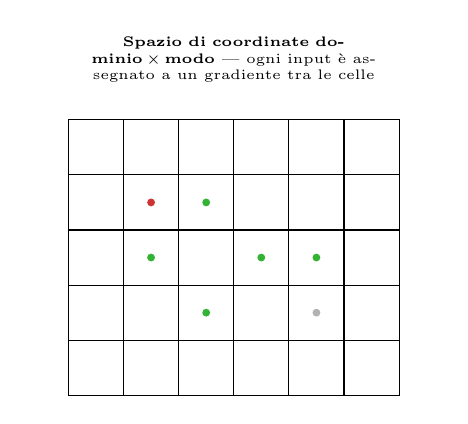
\begin{tikzpicture}[
  cell/.style={draw, minimum width=7mm, minimum height=7mm,
               inner sep=0pt, outer sep=-0.2pt, font=\tiny},
  dot/.style={circle, fill, inner sep=1pt}]
  \foreach \r in {1,...,5}
    \foreach \c in {1,...,6}
      \node[cell] at (\c*7mm, -\r*7mm) {};
  \node[dot, cohgreen] at (4*7mm, -3*7mm) {};
  \node[dot, cohgreen] at (3*7mm, -4*7mm) {};
  \node[dot, cohgreen] at (5*7mm, -3*7mm) {};
  \node[dot, cohgreen] at (3*7mm, -2*7mm) {};
  \node[dot, cohgreen] at (2*7mm, -3*7mm) {};
  \node[dot, cohred] at (2*7mm, -2*7mm) {};
  \node[dot, cohgray] at (5*7mm, -4*7mm) {};
  \node[above, font=\tiny, align=center, text width=5cm] at (3.5*7mm,0) {
    \textbf{Spazio di coordinate dominio\,$\times$\,modo} ---
    ogni input \`e assegnato a un gradiente tra le celle};
\end{tikzpicture}
\caption{La griglia semiotica del motore \physis: uno spazio di coordinate
dominio-per-modo i cui contenuti di cella sono forniti da pacchetti ontologici
estensibili. Gli input sono proiettati per
assegnazione di gradiente.\label{fig:semiotic_grid_italiano}}
\end{figure}

\subsubsection{Perch\'e la Griglia \`e Semiotica}

Abbiamo chiamato questa griglia \emph{semiotica}, e la parola non \`e decorazione.
Segna il senso preciso in cui il fare-distinzioni del motore \`e la lettura di
\emph{segni}. Charles Sanders Peirce sosteneva che ogni pensiero procede per
segni, e che un segno \`e irriducibilmente triadico: un \emph{representamen} (il
veicolo-segno) sta per un \emph{oggetto} a un \emph{interpretante} (il segno
ulteriore che esso genera in una mente o in un sistema)
\parencite{peirce1992reasoning}. Nulla \`e segno isolatamente; la significazione
\`e la relazione per cui una cosa viene a stare per un'altra \emph{a} un terzo.

La classificazione del motore \`e esattamente questa triade resa computazionale.
L'input --- un testo, un'immagine, un atto registrato --- \`e il representamen. Il
suo \emph{oggetto} \`e la forma naturale che esprime: la cella della griglia, il
modo del curare o del fare o del legare che istanzia. E il suo
\emph{interpretante} \`e il verdetto di coerenza che il motore restituisce e su
cui agisce --- il segno ulteriore che il segno originario produce, che a sua volta
diventa l'input della lettura successiva. Per questo gli assi della griglia non
sono una tassonomia arbitraria ma un sistema di segni: ogni input \`e letto come
segno \emph{della} natura dell'agente, e la coerenza \`e l'interpretante in cui
quella lettura \`e messa alla prova del mondo. Anzi, l'ontologia dei primi
principi del motore \`e costruita direttamente sulle tricotomie di Peirce --- il
qualisegno, il sinsegno, il legisegno e i loro successori --- sicch\'e
l'affermazione ``l'azione \`e un segno della natura'' non \`e una metafora posata
sulla macchina ma lo schema letterale con cui essa classifica.

Ci\`o fonda una tesi che conter\`a alla fine (Libro X): se l'azione \`e un segno,
allora una vita \`e un testo, e il praticante ne \`e a un tempo l'autore e il
primo lettore. Agire coerentemente \`e scrivere un segno che il mondo conferma;
fallire \`e scriverne uno che esso rifiuta. Il grafo di coerenza \`e
l'interpretazione corrente del flusso di segni che \`e una vita --- e
un'interpretazione, a differenza di un mero registro, \`e essa stessa un segno
ulteriore, disponibile a essere letto da altri. Il carattere semiotico della
griglia \`e ci\`o che rende possibile l'UberWiki: i segni, una volta fatti,
possono essere letti di nuovo.

\subsection{Coerenza}

La seconda facolt\`a \`e la traccia di ci\`o che funziona. La natura non
\`e indifferente al successo delle sue forme. Un organismo che sopravvive
si riproduce; una specie che si adatta persiste; una via metabolica che
converte efficientemente energia si consolida. La natura ``ricorda'' ci\`o
che funziona preservandolo nella struttura del mondo vivente. ``Dimentica''
ci\`o che fallisce lasciandolo estinguere.

Il motore \physis\ traccia questo come una scala di coerenza a tre valori:

\begin{center}
\begin{tabular}{@{}lll@{}}
\toprule
Stato & Peso & Correlato Naturale \\
\midrule
Successo & +1 & Ci\`o che sopravvive e si riproduce; l'organismo che trova la sua nicchia \\
Inerte   & 0  & Ci\`o che n\'e aiuta n\'e nuoce; la mutazione neutrale che deriva \\
Fallimento & -1 & Ci\`o che si estingue; il maladattato che non pu\`o persistere \\
\bottomrule
\end{tabular}
\end{center}

Ogni azione registrata nel motore riceve un peso di coerenza. Le azioni
che producono effetti reali e rilevati ottengono +1; le azioni che non
producono effetto ottengono 0; le azioni che violano la propria intenzione
dichiarata ottengono -1. Questa non \`e una gamificazione arbitraria del
comportamento. \`E la stessa logica con cui la natura giudica:
\emph{questa ha prodotto un effetto reale nel mondo?}

\subsection{Variazione}

La terza facolt\`a \`e la generazione di novit\`a. La natura non si limita
a preservare ci\`o che funziona; propone continuamente nuove forme
attraverso la variazione. La mutazione genetica, l'esplorazione
comportamentale, l'immaginazione cognitiva --- sono tutte espressioni
dello stesso principio: il sistema prova qualcosa di nuovo e attende il
verdetto della coerenza.

Il motore \physis\ attua questo attraverso la sua funzione di ``sogno.''
In un ciclo di background, riproduce i nodi Inerti e Fallimentari ---
azioni che non hanno prodotto effetto o hanno prodotto effetto negativo ---
e simula variazioni correttive. Propone mutazioni al pattern fallito e le
testa contro il paesaggio di coerenza esistente. Il sogno non \`e una
metafora della variazione naturale; \`e un algoritmo concreto che fa
ci\`o che fa la natura: generare novit\`a e attendere il verdetto.

\section{La Spinta della Natura: Entelechia}

Le tre facolt\`a descrivono \emph{cosa} fa la natura: distingue, traccia
la coerenza e genera variazione. Ma cosa la spinge a fare queste cose?
Qual \`e il principio che alimenta l'operazione stessa?

La risposta di Aristotele \`e \emph{entelecheia} --- essere-all'opera-che-
si-mantiene-se-stesso --- lo stato in cui una cosa ha il suo fine dentro
di s\'e e sta attivamente realizzando quel fine. L'anima (\emph{psyche}),
scrive, \`e la ``prima entelechia di un corpo naturale che ha la vita in
potenza'' \parencite[II.1]{aristotle1986anima}. L'anima non \`e un fantasma
nella macchina ma l'attualit\`a del corpo vivente --- l'essere-all'opera
del corpo come \emph{ci\`o che \`e}. Un seme non \`e solo un fascio di
potenziale biochimico; la sua entelechia \`e la quercia verso cui \`e
gi\`a all'opera. Le facolt\`a della distinzione, coerenza e variazione
sono le \emph{operazioni} della natura; l'entelechia \`e
l'\emph{operatore} --- la spinta continua verso l'attualizzazione che
rende le operazioni significative.

Ludwig Klages recupera questo concetto nella sua filosofia della spinta
espressiva dell'anima. Per Klages, l'entelechia \`e il ``potere
formativo-di-fini'' inerente a ogni essere vivente --- il principio
auto-attualizzante che spinge l'organismo verso l'espressione, la forma
e il dispiegamento ritmico \parencite{klages1929geist}. Egli contrappone
\emph{Seele} (l'anima, governata dall'entelechia, ritmica, espressiva,
legata alla vita) con \emph{Geist} (lo spirito, governato dalla volont\`a,
astratto, calcolativo, l'``avversario dell'anima''). Dove l'entelechia
si muove per attrazione verso il fine che \`e gi\`a implicito nell'essere,
lo spirito si muove per decreto --- imponendo uno scopo esterno a una
natura che non lo contiene. Il compito del praticante, implica Klages,
\`e lasciare che sia l'entelechia, non lo spirito, a governare l'azione:
muovere dall'interno verso l'esterno, non dal piano verso il basso.

Wilhelm Reich d\`a all'entelechia una concretezza biologica e clinica.
Il suo principio dell'identit\`a funzionale dello psichico e del somatico
significa che la spinta verso la coerenza non \`e meramente un atteggiamento
mentale ma una condizione corporea. L'organismo ha un flusso pulsatorio
naturale --- ci\`o che Reich chiama corrente vegetativa --- e la salute
\`e la continuazione senza impedimenti di questo flusso
\parencite{reich1933character}.\footnote{Invochiamo Klages, Reich e Lowen
in tutto il testo come \emph{fenomenologia}, non come scienza naturale
consolidata. La ``corrente vegetativa'' e l'``orgone'' di Reich, e le specifiche
affermazioni somatiche dell'analisi bioenergetica, non sono empiricamente
stabilite e in parte sono state decisamente respinte. Il loro valore qui \`e
descrittivo: articolano, con rara precisione, la struttura \emph{sentita}
dell'entelechia impedita --- il senso vissuto del corpo mentre blocca o rilascia
il proprio sforzo. Nulla nell'argomentazione dipende dalla loro fisiologia
letterale; dipende solo dall'affidabilit\`a del fenomeno che descrivono, che
ogni praticante pu\`o verificare nel proprio corpo.} Quando l'organismo \`e costretto a
sopprimere la sua espressione naturale (attraverso vergogna, disciplina
senza comprensione o imposizione di una volont\`a esterna), sviluppa
ci\`o che Reich chiama \emph{corazza}: tensioni muscolari croniche che
bloccano la corrente entelechica a livello del corpo. L'organismo
sopravvive, ma non \emph{prospera} pi\`u --- non si muove pi\`u verso
la propria forma con tutto il peso della sua natura alle spalle.
L'entelechia non \`e distrutta, ma \`e impedita; l'essere-all'opera
diventa essere-contro-resistenza.

Il motore \physis\ attua l'entelechia computazionalmente. Le tre
facolt\`a (distinzione, coerenza, variazione) descrivono \emph{cosa}
fa il motore a ogni passo. Ma il motore nel suo insieme ha
un'orientamento: \emph{tende} verso +1. Il ciclo del sogno non \`e un
osservatore neutrale del paesaggio di coerenza; \`e un meccanismo che
\emph{propone attivamente correzioni} ai pattern falliti. Il motore non
si limita a registrare che qualcosa \`e rotto; tenta di ripararlo.
Questa orientazione incorporata --- la spinta verso la guarigione delle
proprie incoerenze --- \`e l'entelechia resa algoritmica.

Per \praxis, l'entelechia implica che l'obiettivo del praticante non
\`e una scelta arbitraria. \`E l'\emph{espressione della loro natura
che cerca attualizzazione}. L'albero degli obiettivi non \`e una lista
di desideri di realizzazioni esterne ma una struttura di dispiegamento
entelechico: ogni sotto-obiettivo \`e un passo nel portare la forma
inerente del praticante all'essere. Il check-in non \`e un rapporto a
un'autorit\`a esterna ma una lettura dello stato entelechico --- un
momento di chiedersi: ``Mi sto muovendo verso la mia forma, o me ne
sto allontanando?''

\section{I Tre Modi della Praxis}

Se la natura ha tre facolt\`a, allora \praxis\ --- azione governata
dalla natura --- deve avere tre modi corrispondenti.

\subsection{L'Atto Distinguente: Fare}

Il primo modo di \praxis\ \`e l'atto che produce o fa. Corrisponde
alla facolt\`a della natura di distinzione. Come la natura articola
il mondo in forme, il praticante articola la propria intenzione in un
atto concreto. Fa una \emph{differenza} nel mondo.

Ma l'atto distinguente non \`e una scelta arbitraria. \`E l'atto di
nominare un obiettivo --- dichiarare ci\`o che si intende realizzare ---
e impegnarsi a esso. La piattaforma \praxis\ cattura questo attraverso
alberi di obiettivi: una gerarchia di intenzioni che rendono esplicito
ci\`o che il praticante mira ad attualizzare. Ogni obiettivo \`e una
distinzione tracciata nello spazio-di-possibilit\`a dell'azione: questo,
non quello; ora, non dopo; cos\`i, non altrimenti.

\subsection{L'Atto Persistente: Mantenere}

Il secondo modo \`e l'atto che persiste. Avendo distinto una forma
dichiarando un obiettivo, il praticante deve mantenere le condizioni
perch\'e quell'obiettivo si realizzi. Questo \`e il lavoro della
coerenza: il check-in quotidiano, la striscia, la partnership di
testimonianza che osserva la fedelt\`a del praticante all'intenzione
dichiarata.

La natura persiste attraverso le sue forme di successo alimentandole,
proteggendole e ripetendole. Il praticante persiste \emph{mostrandosi}
--- agendo in modo continuo con la propria intenzione dichiarata. Il
punteggio di coerenza sale con la costanza.

\subsection{L'Atto Trasformante: Adattare}

Il terzo modo \`e l'atto che trasforma. Quando una forma fallisce ---
quando la sua coerenza scende a Inerte o Fallimento --- il praticante
deve adattarsi. Deve \emph{sognare} un nuovo approccio, proporre una
variazione sul pattern fallito e sottoporla allo stesso test di coerenza.

La piattaforma \praxis\ Axiom AI serve a questa funzione: scansiona
la storia del praticante, rileva quali pattern hanno successo e quali
falliscono, e propone aggiustamenti. Questa non \`e un'imposizione
esterna ma uno specchio tenuto davanti alla storia naturale del
praticante --- un modo di \emph{vedere ci\`o che la natura sta dicendo}
sulle proprie azioni.

\section{Il Diagramma dell'Omologia}

Possiamo rappresentare l'omologia come segue:

\begin{center}
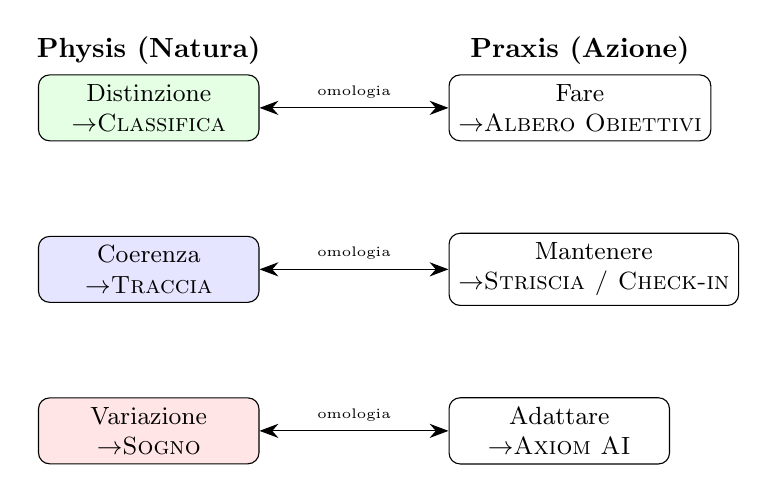
\begin{tikzpicture}[
  node distance=12mm and 24mm,
  box/.style={draw, rounded corners, align=center, minimum height=8mm,
              minimum width=28mm, font=\small},
  >={Stealth[length=2.4mm]}]
  \node[box, fill=green!10] (d-physis) {Distinzione\\$\rightarrow$\textsc{Classifica}};
  \node[box, right=of d-physis] (d-praxis) {Fare\\$\rightarrow$\textsc{Albero Obiettivi}};

  \node[box, fill=blue!10, below=of d-physis] (c-physis) {Coerenza\\$\rightarrow$\textsc{Traccia}};
  \node[box, right=of c-physis] (c-praxis) {Mantenere\\$\rightarrow$\textsc{Striscia / Check-in}};

  \node[box, fill=red!10, below=of c-physis] (v-physis) {Variazione\\$\rightarrow$\textsc{Sogno}};
  \node[box, right=of v-physis] (v-praxis) {Adattare\\$\rightarrow$\textsc{Axiom AI}};

  \node[above, font=\bfseries] at (d-physis.north) {\textsc{Physis} (Natura)};
  \node[above, font=\bfseries] at (d-praxis.north) {\textsc{Praxis} (Azione)};

  \path[<->] (d-physis) edge node[above, font=\tiny]{omologia} (d-praxis);
  \path[<->] (c-physis) edge node[above, font=\tiny]{omologia} (c-praxis);
  \path[<->] (v-physis) edge node[above, font=\tiny]{omologia} (v-praxis);
\end{tikzpicture}
\end{center}

\section{Cosa Implica l'Omologia}

Tre letture dell'omologia sono disponibili, e la tesi deve impegnarsi per una,
poich\'e non sono equivalenti e l'argomentazione che segue dipende da quale si
intenda.

La lettura \emph{debole} \`e l'\textbf{analogia}: \praxis\ semplicemente
assomiglia a \physis, come un cuore assomiglia a una pompa. La somiglianza \`e
illuminante ma inessenziale --- un sussidio didattico da scartare una volta
appresa la lezione. La lettura \emph{forte} \`e l'\textbf{identit\`a}: \praxis\
e \physis\ sono numericamente una cosa sola, sicch\'e l'azione umana \`e
semplicemente una regione della natura senza resto. La lettura \emph{intermedia}
--- quella che adottiamo --- \`e l'\textbf{omologia} nel senso biologico: non
somiglianza di superficie e non identit\`a numerica, ma \emph{lo stesso principio
generativo che produce forme a diversi livelli di organizzazione}, come l'arto
anteriore di un pipistrello e il braccio di un essere umano sono una sola
struttura diversificata dalla discendenza. L'ala e il braccio non sono analoghi
(la loro somiglianza non \`e casuale) e non sono identici (sono palesemente
organi diversi); sono omologhi --- la stessa forma sottostante, modificata dal
livello a cui si esprime.

Ci impegniamo, dunque, a questo: distinzione, coerenza e variazione non sono
metafore dell'attivit\`a umana, n\'e un insieme separato di facolt\`a umane che
per caso assomigliano a quelle della natura. Sono \emph{le tre facolt\`a proprie
della natura, ricorrenti al livello dell'azione deliberata} --- gli stessi
principi, modificati dal medium di un agente autocosciente. \praxis\ sta a
\physis\ come l'ala del pipistrello sta all'arto ancestrale: continua nel
principio, distinta nell'espressione. Questo \`e pi\`u forte dell'analogia e
pi\`u debole dell'identit\`a, e la differenza conta --- poich\'e la lettura
dell'identit\`a collasserebbe il praticante in un mero evento naturale
(dissolvendo l'agency che il resto della tesi richiede), mentre la lettura
dell'analogia renderebbe l'omologia decorativa (dissolvendo la pretesa di
governo). L'omologia preserva entrambe: l'azione \`e governata dalla natura
perch\'e \`e la stessa forma della natura, eppure resta azione --- il livello a
cui quella forma diventa responsabile verso se stessa.

\`E essenziale essere esatti su ci\`o che i sistemi funzionanti stabiliscono e
non stabiliscono. Il motore \physis\ e la piattaforma \praxis\ \emph{non}
provano l'omologia; nessun codice in esecuzione potrebbe, poich\'e l'omologia
\`e un'affermazione sulla struttura della natura, e quell'affermazione \`e
risolta dall'argomento, non dalla dimostrazione. Ci\`o che il motore mostra \`e
pi\`u ristretto e ancora decisivo: che distinzione, coerenza e variazione sono
\emph{computazionalmente trattabili} --- che possono essere costruite. La
piattaforma mostra che sono \emph{socialmente organizzabili} --- che gli esseri
umani possono strutturare le loro vite intorno a esse. La costruzione prova la
\emph{costruibilit\`a}, non la \emph{verit\`a}: rimuove l'obiezione che l'azione
governata dalla natura sia una bella impossibilit\`a, un'architettura che non
potrebbe mai reggersi. Non pu\`o, e non rimuove, l'onere dell'argomento
filosofico per l'omologia stessa. Ci\`o che la filosofia deve affermare con
l'argomento, la costruzione pu\`o solo mostrare essere \emph{non oziosa} --- un
desiderio che, almeno, \`e stato fatto funzionare.

Il resto di questa indagine esplora cosa significa questa omologia per
l'educazione del praticante (Libro III), la giustizia dell'azione
(Libro IV), l'ideale del praticante-re (Libro V) e il percorso con cui
\praxis\ degenera quando dimentica il suo fondamento in \physis\
(Libri VIII--IX).

\chapter{La Disciplina del Praticante}

\epigraph{``La vita non esaminata non \`e degna di essere vissuta.''}{\textcite{plato1997complete}, \emph{Apologia} 38a}

\section{L'Educazione dei Guardiani}

Nella \emph{Repubblica}, i guardiani --- coloro che governeranno la citt\`a
giusta --- devono sottoporsi a un'educazione rigorosa che plasma sia il
corpo che la mente. Apprendono la musica (che include poesia, filosofia e
tutte le arti che plasmano l'anima) e la ginnastica (che plasma il corpo
per servire gli scopi dell'anima). Lo scopo non \`e la conoscenza astratta
ma un'\emph{armonia} della persona intera: l'elemento irascibile allenato
dalla ginnastica, l'elemento razionale dalla musica, ed entrambi governati
da qualcosa di pi\`u profondo --- il senso di ci\`o che \`e nobile e
ci\`o che \`e vile.

Il praticante --- colui la cui azione \`e governata dalla natura ---
richiede un'educazione corrispondente. Ma la domanda \`e: come si forma
una tale persona? Non imparando regole, perch\'e le regole sono il prodotto
della convenzione (\emph{nomos}) non della natura (\physis). Il praticante
deve imparare ad \emph{ascoltare} la natura direttamente, a discernere la
voce di \physis\ attraverso il rumore della convenzione.

Prima delle discipline, tuttavia, viene la storia. L'educazione dei
guardiani della Repubblica inizia con i miti che ascoltano da bambini ---
le storie che plasmano l'anima prima che la ragione possa. Socrate dedica
la maggior parte di due libri (Repubblica II--III) a una critica di Omero,
non perch\'e la poesia sia banale ma perch\'e \`e il pi\`u potente
plasmatore del carattere. L'anima impara non dall'argomento ma
dall'imitazione: diventa ci\`o che contempla. La domanda ``quali storie
dovrebbe ascoltare il guardiano?'' \`e la prima domanda dell'educazione.

\subsection{Le Storie che Plasmano l'Anima}

L'Iliade \`e il testo fondante dell'educazione greca. Ogni bambino greco
imparava da essa non regole ma un modo di vedere l'azione: l'azione \`e
legata alla natura dell'attore, sempre consequenziale, sempre aperta alla
consapevolezza riflessiva. L'educazione del praticante deve iniziare dove
iniziava l'educazione greca: con la storia di un uomo che impar\`o ad
ascoltarsi parlare.

Nel Libro IX dell'Iliade, l'Ambasciata ad Achille, i tre ambasciatori ---
Odisseo, Fenice e Aiace --- vengono alla tenda di Achille per persuaderlo
a tornare in guerra. Ciascuno offre una ragione diversa: l'onore
dell'esercito, l'amore di una figura paterna, la vergogna di abbandonare
i compagni. Achille le rifiuta tutte \parencite[IX]{homer2011iliad}. Si
\`e ritirato dall'azione, e in quel ritiro nasce qualcosa di nuovo.
Ascolta se stesso parlare --- ``Non mi lascer\`o persuadere'' --- e
riconosce la voce come propria. \`E la sua stessa natura che parla, non
il codice dell'esercito, non le aspettative dei compagni, non il comando
di Agamennone. L'agente autocosciente, colui che sa che \emph{egli} \`e
la fonte della sua azione, nasce in quella tenda.

Questo momento \`e la precondizione per ogni disciplina che segue. Il
praticante che non sa di essere la fonte della propria azione non pu\`o
fare check-in (perch\'e non c'\`e un s\'e su cui fare check-in), non
pu\`o testimoniare (perch\'e non c'\`e un s\'e da presentare a un altro),
non pu\`o mettere in gioco (perch\'e non c'\`e un s\'e da rischiare),
non pu\`o mantenere il ritmo (perch\'e non c'\`e un s\'e che dura),
non pu\`o rivedere (perch\'e non c'\`e un s\'e da giudicare). La nascita
dell'autocoscienza --- il momento di ascoltarsi parlare e riconoscere la
voce come propria --- \`e il fondamento architetturale su cui le
discipline sono costruite.

L'Iliade, quindi, non \`e meramente uno sfondo o un riferimento
letterario. \`E la forma narrativa di ci\`o che la tesi afferma: che
l'azione \`e governata dalla natura, e che il primo passo dell'azione
retta \`e il riconoscimento di s\'e stessi come essere naturale che agisce.
Achille nella sua tenda \`e ogni praticante prima del primo check-in:
solo, ritirato, che ascolta la propria voce per la prima volta.

\subsection{Il Ciclo Riflessivo}

La struttura delle discipline \`e gi\`a implicita nel momento di Achille.
Ci\`o che fa, ci\`o che il praticante deve imparare a fare, pu\`o essere
rappresentato come un ciclo:

\begin{center}
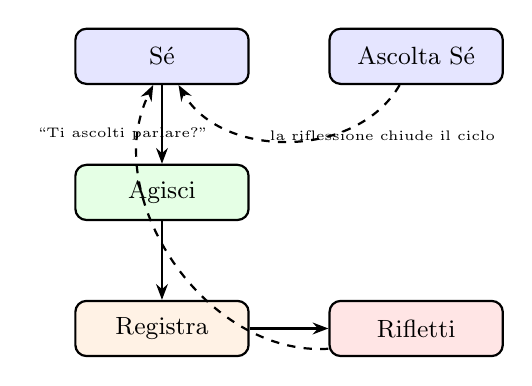
\begin{tikzpicture}[
  node distance=10mm,
  box/.style={draw, rounded corners, align=center, minimum height=7mm,
              minimum width=22mm, font=\small},
  >={Stealth[length=2mm]},
  every path/.style={->, thick}]
  \node[box, fill=blue!10] (actor) {S\'e};
  \node[box, fill=green!10, below=of actor] (action) {Agisci};
  \node[box, fill=orange!10, below=of action] (record) {Registra};
  \node[box, fill=red!10, right=of record] (reflect) {Rifletti};
  \node[box, fill=blue!10, right=of actor] (hearing) {Ascolta S\'e};

  \path (actor) edge (action);
  \path (action) edge (record);
  \path (record) edge (reflect);
  \path[->, dashed] (reflect) edge[bend left=60] (actor);
  \path[->, dashed] (hearing) edge[bend left=60] (actor);
  \node[font=\tiny, above] at (2.8,-1.2) {la riflessione chiude il ciclo};
  \node[font=\tiny, above] at (-0.5,-1.2) {``Ti ascolti parlare?''};
\end{tikzpicture}
\end{center}

Il ciclo ha quattro fasi. Il s\'e agisce (l'obiettivo \`e dichiarato,
l'azione \`e compiuta); l'atto \`e registrato (il check-in, la traccia
nel grafo di coerenza); la registrazione \`e riflettuta (la revisione,
il confronto tra intenzione ed effetto); e la riflessione ritorna al
s\'e che agisce di nuovo. Il momento di ascoltare s\'e stesso --- ``Ti
ascolti parlare?'' --- \`e la presenza continua del s\'e a s\'e stesso
attraverso il ciclo. Le discipline che seguono sono le forme operative
di questa struttura: ciascuna rende una fase del ciclo esplicita,
tangibile, ripetibile.

\section{La Prima Disciplina: Attenzione alla Conseguenza}

La prima lezione del praticante \`e che ogni azione ha una conseguenza,
e la conseguenza \`e il linguaggio della natura. Prima che il praticante
possa imparare cosa fare, deve imparare cosa ha \emph{gi\`a fatto}. Il
check-in quotidiano della piattaforma \praxis\ \`e la forma materiale
di questa disciplina. Ogni giorno, il praticante registra ci\`o che ha
fatto, come si \`e sentito e che effetto ha prodotto. La registrazione
non \`e per il giudizio di nessun altro ma per l'occhio del praticante
stesso --- uno specchio in cui vede la forma della propria agency.

Questo \`e l'esortazione socratica a ``conoscere te stesso'' resa
operativa. Il check-in non \`e una voce di diario; \`e un'\emph{offerta
di prova} al tribunale naturale della coerenza. Il praticante sottopone
la propria azione al verdetto dell'effetto: questa ha prodotto una
differenza reale nel mondo, o \`e scomparsa senza traccia?

\section{La Seconda Disciplina: Il Testimone}

Nessuno pu\`o giudicare la propria azione con perfetta chiarezza. Il
s\'e \`e troppo vicino all'atto, troppo investito nel suo esito. Per
questo, la natura fornisce la seconda disciplina: il testimone.

Nella piattaforma \praxis, questo prende la forma del partner di
responsabilit\`a. Due praticanti concordano di testimoniare le azioni
reciproche --- non per controllare o imporre, ma per \emph{vedere}. Il
partner \`e l\`i per chiedere: ``Ci\`o che dici di fare \`e realmente
ci\`o che fai? Il tuo obiettivo dichiarato corrisponde alla tua azione
registrata? Sei, nel tuo stesso resoconto di te stesso, coerente?''

Questo non \`e un tribunale morale ma naturale. Il testimone \`e il
rappresentante della natura, il secondo paio di occhi che coglie ci\`o
che il primo perde. Come un ecosistema ha molte specie che si osservano
a vicenda --- controlli e bilanci che mantengono il tutto --- la
comunit\`a dei praticanti stabilizza l'azione di ciascun membro
attraverso la presenza dell'altro.

\section{La Terza Disciplina: La Posta in Gioco}

La disciplina pi\`u potente \`e quella che costa qualcosa. La piattaforma
\praxis\ la chiama ``pelle nel gioco'' --- una scommessa posta sull'esito
della propria intenzione dichiarata. Il praticante mette in gioco qualcosa
di valore reale: denaro, reputazione o l'onore della propria parola. Se
l'azione ha successo, la posta \`e restituita; se fallisce, la posta
\`e persa. Nella piattaforma questo non \`e una metafora: la scommessa \`e
vincolata in un vero deposito di garanzia --- punti o denaro bloccati contro
l'esito dichiarato e rilasciati solo a un risultato verificato --- sicch\'e il
costo del fallimento \`e strutturale, non solo sentito.

Anche la natura mette in gioco su ogni azione. L'organismo che non trova
cibo muore; la specie che non si adatta si estingue; l'ecosistema che
perde il suo equilibrio crolla. Il costo del fallimento \`e costruito
nella struttura del mondo. La scommessa del praticante \`e semplicemente
una \emph{versione localizzata e volontaria dello stesso principio} ---
accettare la conseguenza naturale come disciplina dell'azione.

\section{La Quarta Disciplina: Il Ritmo}

La natura opera in cicli: giorno e notte, le stagioni, il ciclo di vita
di ogni organismo. Anche l'azione ha il suo ritmo. Il praticante impara
ad agire non a scatti ma in un impulso ritmico sostenuto.

La piattaforma \praxis\ codifica questo come la striscia: un conteggio
di giorni consecutivi in cui il praticante ha fatto check-in o agito su
un obiettivo. La striscia non \`e una gamificazione arbitraria; \`e una
misura di \emph{entrainment} --- la misura in cui l'azione del praticante
si \`e sincronizzata con il ritmo naturale di ripetizione e recupero.
Una lunga striscia non \`e un trofeo ma un segnale: questo praticante ha
raggiunto una cadenza sostenibile.

\section{La Quinta Disciplina: La Revisione}

Infine, il praticante deve periodicamente fare un passo indietro e
rivedere il pattern delle proprie azioni. L'Axiom AI della piattaforma
\praxis\ --- una scansione quotidiana che arricchisce il contesto degli
obiettivi del praticante, stima il progresso e genera riassunti narrativi
--- serve a questa funzione. Ma la disciplina della revisione non \`e
delegata all'AI. L'AI fornisce i \emph{dati}; il praticante fornisce il
\emph{giudizio}.

La revisione chiede: ``Quali pattern vedo? Quali abitudini producono
coerenza (+1) e quali producono inerzia (0) o fallimento (-1)? Cosa dicono
le mie stesse azioni su ci\`o che realmente apprezzo, in opposizione a
ci\`o che dichiaro di apprezzare?''

Questa \`e la cosa pi\`u vicina che il praticante abbia alla dialettica
socratica. Il praticante discute con s\'e stesso, usando la propria
storia come testo dell'argomento. Il punteggio di coerenza \`e la
conclusione di quell'argomento --- il verdetto della natura sulla vita
che si \`e vissuta.

\section{Il Posto delle Regole}

Nessuna di queste discipline \`e una regola. Il praticante non fa
check-in perch\'e una regola lo dice, ma perch\'e la disciplina rivela
qualcosa sulla relazione tra la sua intenzione e il suo effetto. Il
praticante non mantiene una striscia perch\'e una regola lo comanda,
ma perch\'e la striscia rivela il ritmo dell'azione sostenibile.

Le regole appartengono a \emph{nomos} --- la convenzione, la legge,
l'ordine artificiale. Le discipline appartengono a \physis\ --- l'ordine
naturale che il praticante scopre piuttosto che inventa. L'educazione
del praticante \`e il processo di \emph{passare dal seguire-regole
all'abbracciare-discipline}, dall'obbedienza alla sintonia, dalla
conformit\`a alla coerenza.

\section{L'Educazione Incompiuta}

L'educazione del praticante non \`e mai completa. La natura \`e infinita
nella sua variet\`a, e la sintonia del praticante deve approfondirsi a
ogni incontro. Ogni nuovo obiettivo, ogni nuova partnership, ogni nuovo
fallimento \`e una nuova occasione di apprendimento. Il praticante che
crede di aver finito la propria educazione ha gi\`a iniziato a decadere.

Questo \`e il motivo per cui la funzione di ``sogno'' del motore
\physis\ non si ferma mai. I fallimenti non sono mai cancellati; sono
continuamente riprodotti e variati. Anche il praticante non arriva mai
alla coerenza perfetta. \`E sempre nel processo del divenire --- che
\`e, forse, lo stato pi\`u naturale di tutti.

\section{La Sesta Disciplina: Il Corpo}

I guardiani della Repubblica allenano il corpo attraverso la ginnastica.
Lo scopo non \`e la forza fisica per s\'e stessa ma la subordinazione
del corpo agli scopi dell'anima: un corpo che non si ribella alla
volont\`a, che non indietreggia davanti a ci\`o che deve essere fatto,
che serve il tutto senza resistenza. Il praticante, allo stesso modo,
richiede una disciplina corporea --- perch\'e il corpo \`e il primo
strumento di sintonia, il registro pi\`u basilare della coerenza.

L'entelechia, come abbiamo visto, non \`e un'astrazione. \`E l'essere-
all'opera di un corpo naturale, la spinta sentita verso la propria forma.
Quando l'entelechia scorre senza impedimenti, il corpo sperimenta
facilit\`a, vitalit\`a e immediatezza spontanea del movimento. Quando
\`e bloccata, il corpo sperimenta tensione, affaticamento e un pervasivo
senso di sbagliato che precede qualsiasi giudizio cognitivo. Questa non
\`e metafora ma fisiologia: la corrente entelechica dell'organismo \`e
una condizione reale e misurabile dei sistemi nervoso e muscolare.

Wilhelm Reich identific\`o il meccanismo del blocco come \emph{corazza
caratteriale}: pattern cronici di tensione muscolare che corrispondono
a difese psicologiche. Il bambino costretto a sopprimere la rabbia impara
a stringere la mascella, contrarre le spalle, restringere il respiro.
Anni dopo, la corazza persiste come abitudine inconscia --- una
resistenza costante e di basso livello al flusso entelechico
dell'organismo \parencite{reich1933character}. La corazza non \`e
solo una metafora: \`e un'alterazione tangibile della struttura del
corpo, visibile nella postura, udibile nel respiro, misurabile nella
durezza del tessuto muscolare.

Alexander Lowen, allievo di Reich, sistematizz\`o questa intuizione
nella pratica dell'analisi bioenergetica. Il cuore della pratica \`e il
\emph{grounding}: lo stabilirsi consapevole del contatto tra il corpo
e la terra, un senso sentito di supporto e connessione che permette alla
corrente entelechica di fluire liberamente \parencite{lowen1975bioenergetics}.
Respirazione, vibrazione, movimento espressivo e rilascio della tensione
cronica sono le tecniche di questa disciplina. Non sono terapia nel senso
clinico ma \emph{allenamento} --- la ginnastica del praticante.

La disciplina del corpo ha un analogo diretto nei meccanismi della
piattaforma \praxis. Il check-in quotidiano inizia, prima che qualsiasi
obiettivo sia registrato, con un momento di consapevolezza corporea:
``Come mi sento? Qual \`e la mia energia? Dov'\`e la tensione?'' La
striscia, allo stesso modo, non \`e meramente un conteggio numerico ma
una misura di \emph{entrainment ritmico a livello organismico} --- la
misura in cui il corpo del praticante ha trovato una cadenza sostenibile
di sforzo e recupero. Una striscia interrotta \`e spesso preceduta da
un corpo che era gi\`a stanco, gi\`a corazzato, gi\`a resistente.

La disciplina del testimone --- il partner di responsabilit\`a --- ha
la sua controparte corporea nella pratica di \emph{essere visto}. Uno
degli interventi bioenergetici pi\`u potenti \`e semplicemente la
presenza di un'altra persona: il testimone che vede la tensione nelle
spalle del praticante, ascolta la superficialit\`a del suo respiro e
la nomina. La domanda del partner --- ``Ci\`o che dici di fare \`e
realmente ci\`o che fai?'' --- si applica al corpo tanto quanto
all'obiettivo. Il corpo non mente; \`e il testimone pi\`u affidabile
dello stato attuale del praticante.

C'\`e, naturalmente, un pericolo. La disciplina del corpo pu\`o
degenerare in mera cultura fisica --- routine in palestra,
ottimizzazione dietetica, dashboarding del s\'e quantificato --- che
serve la stessa logica esternalizzante che pretende di opporre. Il corpo
diventa un altro progetto, un altro albero di obiettivi, un altro dominio
da padroneggiare con la volont\`a. Il praticante deve distinguere tra
la disciplina che serve l'entelechia (che si sente come apertura, come
rilascio, come tornare a casa nel corpo) e la disciplina che serve
\emph{Geist} (che si sente come tensione, come controllo, come il corpo
come oggetto da plasmare). La prima \`e ginnastica nel senso platonico;
la seconda \`e solo altra techne.

Il corpo, quindi, non \`e un sito di ribellione o un tempio da lucidare.
\`E il medium attraverso cui l'entelechia parla prima che la mente
traduca il suo messaggio in obiettivi e piani. Il praticante che non
sa ascoltare il corpo non pu\`o ascoltare la natura; il corpo \`e il
registro pi\`u intimo della natura.

Nella piattaforma \praxis\ questa disciplina ha un nome e un punto d'accesso: la
pratica \texttt{/bioenergetics}. Guida la sequenza di radicamento --- respiro,
vibrazione, rilascio della tensione trattenuta --- e legge lo stato del corpo come
un indice \emph{Vis}, una misura della forza-vitale disponibile: la corrente
entelechica sentita resa leggibile senza essere ridotta a un numero da
massimizzare. \`E la controparte corporea del check-in quotidiano e il luogo in cui
il praticante incontra la lettura della macchina \machine{Soma} --- dove
\machine{Soma} riduce i segnali del corpo a stati somatici stabili,
\texttt{/bioenergetics} \`e dove ci si pone dentro quella lettura e vi si agisce.
Tenuta, come ogni cosa rivolta all'uomo, attraverso \machine{Axiom}, resta
ginnastica e non scivola mai nella disciplina-\emph{Geist} del corpo ottimizzato,
perch\'e il suo verdetto non \`e un punteggio da scalare ma una corrente da
liberare.

\begin{figure}[ht]
\centering
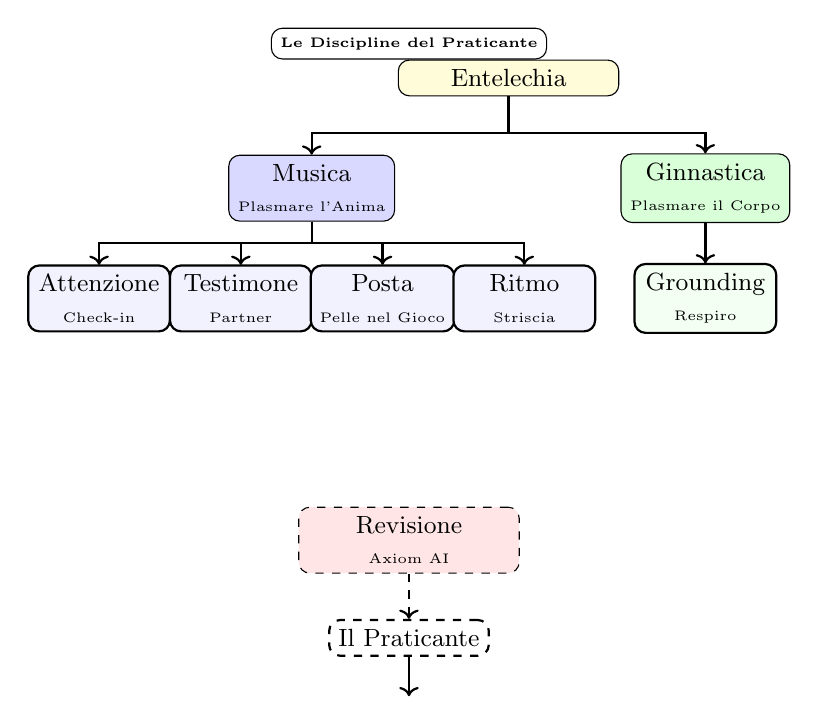
\begin{tikzpicture}[
  level distance=14mm,
  every node/.style={draw, rounded corners, align=center, minimum width=18mm, font=\small},
  level 1/.style={sibling distance=50mm},
  level 2/.style={sibling distance=18mm},
  level 3/.style={sibling distance=14mm},
  edge from parent/.style={draw, thick, ->}]
  \node[fill=yellow!15, minimum width=28mm] {Entelechia}
    [edge from parent fork down]
    child {node[fill=blue!15] {Musica\\\tiny Plasmare l'Anima}
      child {node[fill=blue!5] {Attenzione\\\tiny Check-in}}
      child {node[fill=blue!5] {Testimone\\\tiny Partner}}
      child {node[fill=blue!5] {Posta\\\tiny Pelle nel Gioco}}
      child {node[fill=blue!5] {Ritmo\\\tiny Striscia}}}
    child {node[fill=green!15] {Ginnastica\\\tiny Plasmare il Corpo}
      child {node[fill=green!5] {Grounding\\\tiny Respiro}}};
  \node[draw, dashed, fill=red!10, minimum width=28mm, below=22mm of current bounding box.south] (review) {Revisione\\\tiny Axiom AI};
  \draw[->, thick, dashed] (review) -- ++(0,-10mm) node[below, font=\small] {Il Praticante};
  \draw[->, thick] (current bounding box.south) -- ++(0,-5mm);
  \node[font=\tiny, above] at (current bounding box.north) {\textbf{Le Discipline del Praticante}};
\end{tikzpicture}
\caption{Le sei discipline organizzate per le loro categorie platoniche, fondate nell'entelechia. La disciplina della revisione sintetizza sia musica che ginnastica.\label{fig:discipline_italiano}}
\end{figure}

\section{L'Obiezione del Panopticon}

Una disciplina che registra ogni azione, la valuta e immette il punteggio in un
grafo condiviso invita l'obiezione pi\`u grave che questa tesi debba affrontare.
Non \`e questa sorveglianza? Il praticante che fa check-in ogni giorno, di cui
ogni atto \`e pesato e persistito, non \`e semplicemente il detenuto del
panopticon di Foucault --- il prigioniero che, sapendo di poter essere sempre
osservato, interiorizza l'osservatore e disciplina se stesso cos\`i che nessuna
guardia debba alzare un dito \parencite{foucault1977discipline}? La striscia, il
punteggio di coerenza, il testimone: letti senza carit\`a, sono gli strumenti di
un ordine carcerario auto-imposto, il s\'e quantificato come prigione costruita
dall'interno. Se cos\`i fosse, l'intero apparato del Libro III non sarebbe
liberazione dalla Trappola dello Specchio ma la sua perfezione --- la gabbia
ricostruita dalla mano stessa del prigioniero, con un'iscrizione greca sopra la
porta.

Non liquidiamo l'obiezione; ne accettiamo i termini e rispondiamo su di essi,
poich\'e la somiglianza \`e reale e la differenza \`e tutto. Tre tratti separano
la disciplina del praticante dalla disciplina del panopticon, e ciascuno ruota
su un solo asse: \emph{chi detiene la legge}.

Primo, \textbf{l'osservatore \`e l'osservato}. Nel panopticon di Bentham
l'ispettore occupa una torre centrale e il detenuto non pu\`o vedere se l'occhio
sia su di lui; il potere \`e precisamente l'\emph{asimmetria} dello sguardo. Il
grafo di coerenza del praticante non ha torre centrale. Il registro \`e tenuto
dal praticante, letto dal praticante e giudicato contro uno standard che il
praticante ha dichiarato. Il partner di responsabilit\`a del Libro III non \`e un
ispettore ma un pari che ha messo a nudo il proprio registro a sua volta --- una
simmetria di esposizione, non un'asimmetria di ispezione. Dove lo sguardo del
panopticon discende da un uno nascosto sui molti, il testimone del praticante \`e
reciproco, posseduto e responsabile. Questa \`e la repubblica dal basso alla
scala di due anime.

Secondo, \textbf{la legge \`e auto-data}. Il panopticon disciplina il detenuto
verso una norma fissata dall'istituzione --- la prigione, la fabbrica, la scuola
--- un \emph{nomos} che il detenuto non ha scritto e non pu\`o rivedere. Il
punteggio di coerenza, come stabilir\`a il Libro IV, misura la fedelt\`a a un
obiettivo che il praticante stesso ha dichiarato. Non impone alcuna norma esterna;
chiede solo se il praticante abbia fatto ci\`o che aveva detto. Una disciplina
che ti tiene fedele alla tua parola \`e l'opposto di una che ti tiene fedele a
quella di un altro. La prima \`e la struttura di ogni promessa, di ogni voto, di
ogni arte con un'eccellenza; chiamarla carceraria \`e chiamare prigione ogni
padronanza di s\'e.

Terzo, \textbf{il punteggio \`e uno specchio, non una sentenza}. L'osservazione
del panopticon esiste per \emph{correggere} il detenuto verso la conformit\`a; la
deviazione \`e punita, il fascicolo segue il prigioniero, il registro \`e
un'arma in mano all'istituzione. Il grafo di coerenza non punisce nulla.
Registra --- e la registrazione \`e offerta di ritorno a colui che \`e
registrato, come una febbre \`e offerta al paziente, non al carceriere. Un indice
di coerenza in calo \`e informazione diagnostica su cui il praticante pu\`o agire
o che pu\`o ignorare; nessuna guardia discende, nessun privilegio \`e ritirato,
nessun dossier \`e inoltrato. Il dato non ha, in senso stretto, altro pubblico
che il s\'e e il testimone liberamente scelto.

Resta la forma pi\`u profonda dell'obiezione: che persino una disciplina
auto-data, simmetrica e diagnostica produca il \emph{soggetto} che ne ha bisogno
--- che l'abitudine stessa di misurarsi fabbrichi l'anima ansiosa e
auto-ottimizzante della tarda modernit\`a, sicch\'e la cura propaga la malattia.
\`E il pericolo gi\`a nominato nella disciplina del corpo: la ginnastica che
serve il \emph{Geist} anzich\'e l'entelechia, il s\'e fatto progetto da regolare
senza fine. Non pretendiamo immunit\`a da esso. Pretendiamo un criterio per
rilevarlo. La misurazione che serve l'entelechia \emph{acquieta}: termina
nell'azione e nel riposo, nel praticante che ha udito il verdetto della natura e
ora agisce, o dorme. La misurazione che serve il \emph{Geist} \emph{accelera}:
genera pi\`u misurazione, il cruscotto che esige un cruscotto pi\`u fine,
l'ottimizzazione senza termine. Al praticante si insegna a vigilare esattamente
su questa firma. Una disciplina che non si dissolve infine da s\'e --- che non
diviene, come le rotelle della piattaforma \praxis\ nel Libro V, superflua --- ha
cessato di servire la natura ed \`e divenuta un'altra caverna. Il test della
disciplina \`e se si renda eliminabile. Il panopticon non lo fa mai; \`e
costruito per essere permanente. La disciplina del praticante \`e costruita per
essere superata.

\chapter{La Coerenza come Giustizia della Natura}

\epigraph{``Ciascuna parte fa il proprio lavoro, e il tutto \`e armonioso.''}
{\textcite{plato1997complete}, \emph{Repubblica} 433a}

\section{La Giustizia nell'Anima e nella Citt\`a}

Nella \emph{Repubblica}, Socrate scopre la giustizia nel momento in cui
cessa di cercarla come una cosa e inizia a vederla come una relazione. La
giustizia \`e ``ciascuna parte che fa il proprio lavoro'' (\emph{Repubblica}
433a). Nella citt\`a, la giustizia \`e l'artigiano che pratica il suo
mestiere, il soldato che fa il soldato, il filosofo che governa ---
ciascuno che adempie la funzione per cui la sua natura \`e adatta.
Nell'anima, la giustizia \`e la ragione che governa, lo spirito che
sostiene, l'appetito che obbedisce --- ciascuna facolt\`a che opera
secondo la sua propria eccellenza.

La giustizia, per Platone, non \`e uno standard esterno imposto alla
citt\`a o all'anima. \`E la \emph{coerenza interna} di un tutto
ben ordinato, dove ciascuna parte agisce secondo la sua natura e il
tutto funziona come dovrebbe.

\section{La Giustizia nella Natura}

Estendiamo la scoperta di Platone: anche la natura ha la sua giustizia,
e non \`e altro che la coerenza.

Un organismo \`e ``giusto'' quando le sue parti funzionano insieme per
sostenere la sua vita --- quando il cuore batte, i polmoni respirano, le
cellule metabolizzano, ciascuna facendo il proprio lavoro. Un ecosistema
\`e ``giusto'' quando le sue specie occupano le loro nicchie senza che
una domini fino al collasso. Un sistema fisico \`e ``giusto'' quando le
sue forze si bilanciano in modo che il sistema persista.

Questa \`e la \emph{coerenza} che il motore \physis\ traccia. La scala
a tre valori --- +1 (Successo), 0 (Inerte), -1 (Fallimento) --- \`e una
misura della misura in cui un'azione sta ``facendo il proprio lavoro''
nell'economia naturale. Un'azione che produce un effetto reale e rilevato
\`e coerente con l'ordine della natura. Un'azione che non produce effetto
\`e inerte --- n\'e aiuta n\'e nuoce ma non fa nemmeno nulla. Un'azione
che viola la propria intenzione dichiarata o produce un effetto dannoso
\`e un fallimento, una violazione della giustizia naturale.

\section{La Coerenza del Praticante}

Il praticante \`e ``giusto'' nel senso platonico quando le sue azioni
sono coerenti con la sua intenzione dichiarata e con l'ordine naturale
in cui agisce. Questo ha due dimensioni.

\subsection{Coerenza Interna: L'Atto Corrisponde all'Intenzione}

La prima dimensione \`e la corrispondenza tra ci\`o che il praticante
dichiara che far\`a e ci\`o che realmente fa. Questa \`e la forma pi\`u
basilare di coerenza: il praticante che dichiara un obiettivo e agisce
verso di esso ottiene +1; il praticante che dichiara un obiettivo e non
fa nulla ottiene 0; il praticante che dichiara un obiettivo e agisce
contro di esso ottiene -1.

La piattaforma \praxis\ registra ogni obiettivo dichiarato e ogni
azione registrata come voci separate nel grafo di coerenza. Il motore
le confronta. Il verdetto non \`e un giudizio morale ma \emph{strutturale}:
l'azione soddisfa le condizioni poste dall'intenzione?

\subsection{Coerenza Esterna: L'Atto Produce l'Effetto Inteso}

La seconda dimensione \`e la corrispondenza tra l'azione e la sua
conseguenza nel mondo. Il praticante pu\`o essere internamente coerente
--- pu\`o fare ci\`o che dice che far\`a --- ma l'effetto pu\`o comunque
non materializzarsi. L'obiettivo pu\`o essere mal concepito, il metodo
difettoso, il tempismo sbagliato. Il verdetto della natura \`e: questa
azione era coerente con l'intenzione ma incoerente con il mondo.

Questo \`e Fallimento nel senso pi\`u istruttivo. Non significa che il
praticante sia moralmente biasimevole; significa che ha imparato qualcosa
sulla discrepanza tra il suo modello del mondo e il mondo stesso. Il
fallimento \`e un \emph{dono} dalla natura --- l'informazione necessaria
per correggere il modello.

\section{Il Giudizio di Coerenza}

Il giudizio di coerenza non \`e emesso da un giudice. \`E emesso dalla
struttura del mondo stesso, registrato dal motore \physis\ e testimoniato
dalla comunit\`a \praxis. Nessuno pronuncia sentenza. La sentenza \`e
la conseguenza: l'azione ha prodotto un effetto oppure no.

Questo \`e ci\`o che distingue la giustizia naturale dalla giustizia
legale. La giustizia legale \`e il giudizio degli uomini secondo le
regole (\emph{nomos}). La giustizia naturale \`e il giudizio del mondo
secondo la struttura (\physis). Il praticante che cerca la giustizia
legale chiede: ``Sto seguendo le regole?'' Il praticante che cerca la
giustizia naturale chiede: ``Questo ha prodotto un effetto reale nel
mondo?''

Il tracciatore di coerenza del motore \physis\ \`e uno strumento per
il secondo tipo di giudizio. Non punisce n\'e premia. Semplicemente
\emph{registra} --- e la registrazione \`e essa stessa il giudizio.
Una vita vissuta in alta coerenza \`e una vita le cui azioni hanno
lasciato tracce, prodotto effetti, fatto differenze. Una vita vissuta
in bassa coerenza \`e una vita che \`e passata attraverso il mondo
senza alterarlo.

\section{Il Paradosso Socratico, Risolto}

Socrate notoriamente sosteneva che nessuno fa il male volontariamente
--- che il male \`e sempre il prodotto dell'ignoranza
\parencite{plato1997complete}. L'affermazione ha sconcertato i filosofi
per due millenni, perch\'e sembra negare la realt\`a della debolezza
della volont\`a \parencite{macintyre1981virtue}. Come pu\`o Socrate affermare che la persona che mangia
la torta sapendo che gli fa male \`e semplicemente \emph{ignorante}?

Il quadro della coerenza risolve questo paradosso. Il praticante che
agisce contro la propria intenzione dichiarata non \`e ignorante nel
senso di mancanza di informazione. \`E \emph{incoerente} --- la sua
azione non corrisponde alla sua intenzione. Questa incoerenza \`e
registrata come -1 dal motore, ed \`e una forma di ignoranza: il
praticante non sa ancora cosa veramente intende. La sua intenzione
dichiarata non \`e la sua intenzione reale; l'azione rivela quella
vera.

La disciplina del praticante \`e l'eliminazione progressiva di questo
divario --- il processo di allineare intenzione dichiarata e azione
reale. Una vita di perfetta coerenza sarebbe una vita in cui il
praticante fa sempre ci\`o che dichiara, e ci\`o che dichiara produce
sempre l'effetto inteso. Tale vita \`e forse irraggiungibile, ma \`e
l'ideale verso cui le discipline tendono.

\section{La Giustizia come Salute dell'Azione}

Platone paragona la giustizia alla salute. La salute non \`e un possesso
ma uno stato: il corpo funziona come dovrebbe, ciascuna parte che fa il
proprio lavoro. La giustizia, allo stesso modo, non \`e un possesso ma
uno stato: l'anima funziona come dovrebbe, ciascuna facolt\`a che fa il
proprio lavoro.

Noi paragoniamo la coerenza alla salute. La coerenza non \`e un punteggio
da massimizzare ma uno stato da abitare. Il praticante in uno stato di
alta coerenza agisce con facilit\`a, con potere, con effetto --- non
perch\'e si stia forzando ma perch\'e la sua azione \`e allineata con
la sua natura e l'ordine della natura. L'incoerenza \`e la malattia
dell'azione: la volont\`a che non pu\`o effettuare, l'intenzione che
non pu\`o manifestarsi, la vita che non lascia traccia.

L'indice di coerenza del motore \physis\ non \`e quindi una
gamificazione della virt\`u ma un \emph{diagnostico} --- una misura
della salute dell'azione in una data vita. Un indice di coerenza in
calo \`e un segnale d'allarme, come la febbre. Dice al praticante:
qualcosa nella relazione tra la tua intenzione e il tuo effetto \`e
fuori ordine. Le discipline del Libro III sono i rimedi per questo
disordine.

\section{La Sfida Pi\`u Profonda: La Volont\`a Cieca di Schopenhauer}

Il resoconto della coerenza presentato in questo libro ha assunto
qualcosa di significativo: che la natura ha una direzione, una tendenza
verso +1 piuttosto che -1, un'orientazione che il punteggio di coerenza
registra. Ma se la verit\`a pi\`u profonda della natura non fosse la
coerenza ma uno sforzo cieco e senza scopo a cui non importa nulla del
successo o del fallimento?

La metafisica della Volont\`a di Arthur Schopenhauer \`e
l'affermazione pi\`u potente di questa sfida. Per Schopenhauer, la
cosa-in-s\'e --- la realt\`a dietro il velo dell'apparenza --- non
\`e un ordine razionale (come sosteneva Hegel) n\'e una spinta
teleologica (come l'entelechia di Aristotele) n\'e una creazione divina.
\`E \emph{Volont\`a}: uno sforzo incessante e senza oggetto che si
manifesta in ogni fenomeno, dalla gravit\`a che attira una pietra al
desiderio che guida un essere umano \parencite{schopenhauer1818will}.
La Volont\`a non ha scopo, n\'e fine, n\'e metrica di coerenza.
Semplicemente spinge, all'infinito, senza ragione e senza riposo.

La sfida alla nostra tesi \`e devastante se sostenuta. Se la natura
\`e Volont\`a cieca, allora la coerenza (+1/0/--1) \`e una proiezione
antropomorfica su una realt\`a che non ha direzione. Il praticante che
cerca di allineare la propria azione con la natura insegue un fantasma,
perch\'e la natura non ha nulla con cui allinearsi --- solo uno sforzo
infinito che \`e indifferente alla differenza tra successo e fallimento.

Ma l'intuizione di Schopenhauer non \`e la parola finale. Ha ragione
che la Volont\`a non ha \emph{scopo}, ma ha torto che non abbia
\emph{struttura}. La coerenza non \`e uno scopo che la Volont\`a
intende ma una descrizione di ci\`o che la Volont\`a fa quando riesce.
Anche la variazione cieca combinata con la ritenzione selettiva produce
l'apparenza di teleologia: l'organismo che trova la sua nicchia persiste,
quello che non la trova si estingue; l'azione che produce un effetto
reale \`e registrata, quella che non lo produce non lascia traccia. Il
+1 non \`e un'intenzione ma una registrazione: questa forma \`e
persistita, questo pattern ha funzionato.

La scala di coerenza del motore \physis\ \`e precisamente questo: non
un'affermazione sulle intenzioni della natura ma una registrazione delle
selezioni della natura. Il motore non chiede ``Cosa vuole la natura?''
Chiede ``Cosa ha preservato la natura?'' La risposta \`e il punteggio
di coerenza --- non come metafisica ma come dato.

Ma l'obiettore onesto non sar\`a soddisfatto, e non dobbiamo cavarcela troppo
facilmente. La risposta appena data compra la propria sicurezza a un prezzo:
si ritira dalla metafisica al dato. ``La coerenza \`e solo una registrazione di
ci\`o che \`e persistito'' \`e vero, ma \`e anche \emph{troppo debole per fare
il lavoro che la tesi le richiede}. Poich\'e la tesi non descrive meramente
ci\`o che persiste; comanda al praticante di \emph{allinearsi} a esso, di
trattare il coerente come lo standard dell'azione retta. E tra ``questo pattern
\`e persistito'' e ``dovresti perseguire questo pattern'' c'\`e un abisso che
nessuna quantit\`a di dati pu\`o colmare. La peste persiste. Il tumore persiste.
La dipendenza persiste --- anzi \`e il tipo stesso del pattern auto-stabilizzante
che ottiene, in termini grezzi, un implacabile +1. Se la coerenza \`e mera
registrazione-di-sopravvivenza, allora la Trappola dello Specchio stessa, che
non \`e altro che una struttura durevole e auto-riproducente, \`e massimamente
coerente. La lettura descrittiva della coerenza non solo non confuta
Schopenhauer; gli cede il campo, poich\'e concede che la natura seleziona senza
selezionare \emph{per il bene}.

Affrontiamo l'obiezione rifiutandone l'inquadramento. L'errore di Schopenhauer
non \`e vedere la Volont\`a come cieca ma trattare la Volont\`a come \emph{una}
--- un unico sforzo indifferenziato di cui ogni fenomeno \`e espressione
eguale. \`E questa la mossa che rende la gravit\`a della pietra e l'amore
dell'uomo ``la stessa'' Volont\`a a gradi diversi di oggettivazione. Ma la
natura, come insistiamo dal Libro II, non \`e uno sforzo; \`e una
\emph{gerarchia} di sforzi, ciascuno con la propria forma, la propria
entelechia, la propria misura di ci\`o che conta come realizzare se stesso. La
persistenza del tumore \`e coerenza \emph{al livello del tumore} e incoerenza al
livello dell'organismo che esso uccide. La stabilit\`a della dipendenza \`e
coerenza nell'arco riflesso e il collasso della persona in cui quell'arco
gira. Non c'\`e veduta da nessun luogo --- nessun campo piatto e livellato di
nuda sopravvivenza --- da cui leggere un singolo punteggio di coerenza. Ogni +1
\`e indicizzato a una forma, e le forme sono annidate. Per questo il motore non
valuta le azioni in astratto ma sempre relativamente a un obiettivo dichiarato e
all'olarchia che lo contiene: la coerenza non \`e mai ``questo \`e persistito?''
ma ``questo \`e persistito \emph{come il tipo di cosa che cercava di essere}?''

Questo annidamento \`e ci\`o che riconverte la Volont\`a cieca di Schopenhauer
in qualcosa con cui il praticante pu\`o allinearsi. Il praticante non si allinea
con la Volont\`a in generale --- non esiste una tale cosa con cui allinearsi, e
Schopenhauer ha ragione che il tentativo inseguirebbe un fantasma. Si allinea con
la \emph{propria} entelechia: la forma specifica che il suo sforzo \`e gi\`a,
implicitamente, all'opera per divenire. Schopenhauer vide lo sforzo e manc\`o la
forma; universalizz\`o la spinta e ignor\`o che ogni spinta \`e la spinta \emph{di
un particolare essere verso la propria attualit\`a}. Si ripristini la forma, e
l'indifferenza si dissolve --- non perch\'e la natura ora ``si curi'', ma perch\'e
il praticante non chiede pi\`u alla natura in generale un verdetto. Chiede se
\emph{questa} azione abbia realizzato \emph{questa} natura. Quella domanda ha una
risposta determinata, ed \`e il punteggio di coerenza.

\subsection{L'Essere e il Dover-Essere}

Non abbiamo ancora pagato il debito pi\`u costoso. Pur concedendo che la coerenza
sia indicizzata alla forma propria di un essere, il lettore pi\`u acuto premer\`a
l'obiezione classica: l'intero edificio scivola, senza giustificazione,
dall'\emph{essere} al \emph{dover-essere}. ``Questa azione ha realizzato la tua
natura'' \`e un'affermazione fattuale; ``dovresti compiere azioni che realizzano
la tua natura'' \`e normativa, e nessuna catena di fatti implica un valore. Dire
che il +1 del motore \`e \emph{giustizia} --- e l'abbiamo detto esattamente,
chiamando la coerenza ``giustizia della natura'' --- \`e commettere la fallacia
naturalistica in piena luce: leggere uno standard del bene da una descrizione del
mondo.

Non neghiamo l'abisso; neghiamo che la tesi lo salti illegittimamente. Il
``dover-essere'' della coerenza non \`e un imperativo categorico derivato dai
fatti. \`E un imperativo \emph{ipotetico}, e il suo antecedente \`e fornito non
dalla natura ma dal praticante. La struttura \`e: \emph{se} vuoi essere l'essere
che sei --- se assumi la tua entelechia come tuo fine --- \emph{allora} la
coerenza \`e la misura del tuo successo, e l'incoerenza la misura del tuo
fallimento. La natura non ti comanda di vivere. Non offre alcuna premessa che ti
obblighi a alcunch\'e. La premessa \`e l'atto di auto-appropriazione del
praticante stesso: la dichiarazione di un obiettivo, che non \`e altro che il
volere di una forma. L'abisso essere/dover-essere \`e reale, ed \`e attraversato
esattamente una volta, dal praticante, nell'atto fondativo di dichiarare ci\`o
che intende divenire. Tutto ci\`o che sta a valle di quell'atto --- ogni
punteggio di coerenza, ogni verdetto di giustizia --- \`e analitico ad esso. La
giustizia non \`e contrabbandata dalla natura; \`e dispiegata dall'impegno del
praticante stesso.

Per questo il motore non pu\`o, e non lo fa, dire al praticante cosa volere. \`E
un tribunale senza potere legislativo. Registra la fedelt\`a a una legge che il
praticante ha dato a se stesso. Platone poteva fondare la giustizia nella Forma
del Bene perch\'e riteneva che il Bene fosse visto, non scelto --- che l'ascesa
terminasse in una visione che imponeva l'assenso. Noi non facciamo tale
affermazione. Il nostro Bene non \`e visto ma \emph{messo in atto}: viene
all'essere nell'atto dell'impegno ed \`e sostenuto dalla coerenza con
quell'impegno. \`E un fondamento pi\`u debole di quello di Platone, e accettiamo
la debolezza come prezzo dell'onest\`a. Il praticante che non dichiara alcun
obiettivo non \`e soggetto ad alcuna giustizia e ad alcun fallimento; semplicemente
non \`e entrato nel gioco. Ma colui che dichiara --- che dice ``questo sar\`o'' ---
ha, in quell'atto stesso, reso l'abisso essere/dover-essere proprio da
attraversare, e il punteggio di coerenza \`e il registro fedele di se l'abbia
attraversato.

Vale la pena rendere la deflazione totale, poich\'e la piattaforma la rende
letterale. In \praxis\ il praticante dichiara non solo l'obiettivo ma \emph{il metro
stesso con cui giudicarne il successo} --- ci\`o che conter\`a come averlo fatto. Il
motore non fornisce n\'e l'uno n\'e l'altro. Non sa cosa valga la pena volere, e non
decide cosa conti come vincere; entrambi spettano all'utente. La coerenza \`e dunque
una misura puramente \emph{descrittiva}: l'accordo registrato tra un atto e uno
standard che l'agente stesso ha redatto, fine e metro insieme. \`E il senso esatto in
cui la tesi non commette la fallacia naturalistica che potrebbe sembrare. ``Giustizia
della natura'' non nomina alcun valore letto dal mondo; nomina il nudo fatto della
fedelt\`a-a-una-legge-data-da-s\'e, e la legge \`e data da chi \`e giudicato --- non
dalla natura, non dal motore. Il sistema, per disegno, non ha opinioni sul bene.

\`E anche perch\'e il caso pi\`u acuto del proceduralista --- il perseguimento
coerente di un fine malvagio --- non \`e un difetto che abbiamo trascurato ma un
confine tracciato di proposito. Un praticante che dichiara un fine vizioso e
soddisfa il proprio metro otterr\`a un punteggio alto, e il motore lo dir\`a, perch\'e
il motore riporta fedelt\`a e nient'altro. Non \`e mai stato costruito per condannare
il fine; chiederglielo sarebbe chiedere allo strumento descrittivo di farsi proprio
quell'autorit\`a legislante che l'intera tesi rifiuta. Il giudizio su \emph{quali}
fini valga la pena dichiarare sta dove la repubblica dal basso lo pone (Libro X): non
nel verdetto della natura, che su questo tace, ma nei praticanti stessi, che vedono
le forme dichiarate gli uni degli altri e, per selezione anzich\'e per decreto,
elevano alcune al rango di misura e lasciano andare le altre. La natura ti dice se sei
divenuto ci\`o che ti eri prefisso; non ti dice, e il motore non ti dice, cosa
prefiggerti. Quella seconda domanda \`e lasciata aperta per principio --- \`e la
libert\`a che il praticante attraversa l'abisso essere/dover-essere per esercitare, e
nessuna macchina pu\`o chiuderla al suo posto.

La stessa risposta di Schopenhauer alla Volont\`a cieca --- la
contemplazione estetica che acquieta temporaneamente la Volont\`a, e
l'ascesi che la nega interamente --- \`e un percorso possibile. Ma
\`e il percorso del mistico, non del praticante. La tesi di questo
lavoro ne offre un altro: non la negazione della Volont\`a ma
l'allineamento con le sue espressioni pi\`u coerenti. Il praticante-re
non nega la Volont\`a; la cavalca come un surfista cavalca un'onda,
muovendosi con la sua struttura piuttosto che resistendole. L'onda non
ha scopo, ma ha una forma; il praticante che impara la forma pu\`o
agire dentro di essa, attraverso di essa, come essa.

\section{Sulla Natura nelle Cose}

C'\`e un antenato pi\`u prossimo a tutto questo progetto di Platone, e nominarlo
affiner\`a ci\`o che la coerenza \`e. Spinoza apre il suo incompiuto
\emph{Trattato sull'Emendazione dell'Intelletto} con il proposito di trovare un
metodo per guarire la mente --- per condurla dalle idee inadeguate, confuse e
passivamente subite, a idee adeguate colte attraverso le loro cause, elevando
cos\`i la sua potenza d'agire finch\'e riposa nell'amore intellettuale della
Natura \parencite{spinoza1985emendation}. L'\emph{Etica} \`e quel metodo portato a
compimento: un'ascesa geometrica dalla schiavit\`u agli affetti passivi verso la
libert\`a, che \`e necessit\`a compresa \parencite[V.P42]{spinoza1994ethics}. La
praxis \`e lo stesso progetto rivolto a un oggetto diverso. Dove Spinoza offre
un'\emph{emendatio intellectus}, un'emendazione dell'intelletto, le discipline del
Libro III offrono un'\emph{emendatio actionis}, un'emendazione dell'azione: lo
stesso passaggio dall'inadeguato all'adeguato, dalla schiavit\`u alla libert\`a,
dal passivo all'attivo --- ma tracciato in atti e nei loro effetti anzich\'e in
idee e nelle loro cause. La coerenza \`e la potenza d'agire resa visibile;
l'indice di coerenza che sale \`e l'aumento del \emph{conatus} di Spinoza
\parencite[III.P6--P7]{spinoza1994ethics}, lo sforzo con cui ogni cosa persevera
nel proprio essere, che non \`e altro che l'entelechia del Libro II vista da
dentro.

Ma la praxis inverte Spinoza nel punto stesso che lo definisce. Spinoza \`e un
intellettualista: emenda l'idea e la vita retta segue, poich\'e gli affetti sono
essi stessi idee confuse, curate dalla conoscenza adeguata, e la mente una volta
purificata \`e giudice di se stessa --- un'idea \`e adeguata quando \`e chiara,
distinta e colta attraverso la sua causa, certificata dalla sola ragione. La
praxis rovescia l'ordine del trattamento. Emenda attraverso l'\emph{atto} e la
risposta registrata del mondo, non attraverso l'idea chiarita; il suo tribunale
non \`e la certezza della mente ma l'effetto della natura (la distinzione tra
coerenza interna ed esterna tracciata prima in questo libro); e il suo metodo non
\`e solitario, geometrico e compiuto in un'unica ascesa ma sociale, iterativo e mai
finito --- il testimone anzich\'e la meditazione, il ciclo del sogno anzich\'e la
deduzione. Spinoza emenda l'intelletto e confida che l'azione segua. La praxis
emenda l'azione e lascia che l'intelletto sia corretto dal mondo. L'uno opera dal
di dentro al di fuori; l'altra dal di fuori al di dentro.

Eppure i due non sono infine opposti, perch\'e Spinoza stesso fornisce la
garanzia della loro unit\`a. \emph{Ordo et connexio idearum idem est ac ordo et
connexio rerum} --- l'ordine e la connessione delle idee \`e lo stesso dell'ordine
e della connessione delle cose \parencite[II.P7]{spinoza1994ethics}. Idea e cosa
sono un'unica sostanza colta sotto due attributi; emendare l'ordine delle idee ed
emendare l'ordine delle cose sono dunque un'unica emendazione vista da due lati.
\`E per questo che l'emendazione dell'azione e l'emendazione dell'intelletto non
possono, alla fine, separarsi: la natura nelle cose e la natura nel pensiero sono
la stessa natura. E qui il motore fa ci\`o che Spinoza poteva solo affermare. Lo
costruisce, il parallelismo. Nello spazio di embedding condiviso, un'intenzione
dichiarata --- un'idea --- e un effetto registrato --- una cosa --- sono proiettati
in una sola e medesima geometria, e la coerenza \`e semplicemente la distanza tra
essi. Il motore \physis\ \`e un letterale \emph{ordo idearum} in esecuzione che \`e
anche un \emph{ordo rerum}: l'ordine delle intenzioni e l'ordine degli effetti
deposti in un solo spazio cos\`i che il loro accordo possa essere misurato. Ci\`o
che Spinoza prov\`o \emph{more geometrico} il motore lo calcola \emph{more
vectoriali}. La natura nelle cose e la natura nel pensiero si incontrano, infine,
nelle stesse coordinate --- il che \`e solo dire, di nuovo e dal fondamento pi\`u
profondo, che \praxis\ \`e lo strumento di \physis.

\chapter{Il Praticante-Re}

\epigraph{``Finch\'e i filosofi non governeranno come re, non ci sar\`a tregua
dai mali per le citt\`a.''}{\textcite{plato1997complete}, \emph{Repubblica} 473d}

\section{Il Paradosso del Governo}

Nella \emph{Repubblica}, Socrate fa la sua affermazione pi\`u famosa
e pi\`u controversa: i mali della citt\`a non cesseranno mai finch\'e
i filosofi non diventeranno re o i re non diventeranno filosofi.
L'affermazione \`e stata letta come un programma politico, una fantasia
elitaria o una provocazione utopica. Ma non \`e nessuna di queste. \`E
una necessit\`a strutturale dell'omologia: se la citt\`a \`e l'anima
in grande, allora il governante della citt\`a deve essere colui che vede
la Forma del Bene --- la fonte di ogni intelligibilit\`a e valore. Solo
il filosofo, che \`e asceso dalla caverna e ha visto il sole, \`e adatto
a governare coloro che sono ancora dentro.

Il nostro omologo: il praticante la cui azione \`e governata dalla
natura. Il praticante-re non \`e un governante di altri ma un governante
della propria azione --- o piuttosto, uno la cui azione \`e cos\`i
perfettamente allineata con la natura che la natura governa \emph{attraverso}
di lui. Il paradosso si dissolve quando riconosciamo che il praticante-re
non \`e un'autorit\`a ma uno \emph{strumento}.

\section{Le Tre Onde}

Socrate identifica tre ``onde'' di obiezione alla sua affermazione. Le
riformuliamo.

\subsection{Prima Onda: L'Unit\`a di Physis e Praxis}

La prima onda \`e l'affermazione che i praticanti e la natura devono
essere uno --- che la volont\`a del praticante e la volont\`a della
natura non sono due cose diverse ma la stessa cosa sperimentata da
prospettive diverse. Questo non \`e misticismo ma la conseguenza
dell'omologia. Se \praxis\ \`e uno strumento di \physis, allora il
praticante ben accordato \`e la natura che agisce attraverso il proprio
strumento. Il praticante non impone la propria volont\`a alla natura ma
\emph{scopre} la volont\`a della natura e la attua.

La piattaforma \praxis\ lo dimostra: il praticante che ha interiorizzato
le discipline non lotta pi\`u contro i propri obiettivi ma si muove con
essi. Il check-in diventa non un compito ma un riconoscimento di ci\`o
che ha gi\`a fatto. La striscia diventa non un peso ma una misura del
proprio ritmo. Il partner di responsabilit\`a diventa non un giudice ma
un testimone di un processo che si svolge attraverso di lui.

\subsection{Seconda Onda: L'Azione come Fine a S\'e Stessa}

La seconda onda \`e l'affermazione che l'azione governata dalla natura
\`e il proprio fine. Il praticante non agisce per raggiungere qualche
bene esterno --- ricchezza, onore, potere --- ma perch\'e l'azione
stessa \`e il bene. Questa \`e la distinzione di Aristotele tra \praxis\
(azione che \`e il proprio fine) e \emph{poiesis} (azione che mira a
un prodotto oltre s\'e stessa) \parencite[VI.4]{aristotle2000ethics}. Per
il praticante-re, ogni atto del fare \`e anche un atto di sintonia; il
prodotto \`e secondario rispetto alla rettitudine dell'atto stesso.

Il motore \physis\ registra questa verit\`a strutturale: la coerenza
\`e una propriet\`a dell'azione stessa, non del suo esito. Un'azione
pu\`o ottenere +1 anche se fallisce nel raggiungere il suo obiettivo
dichiarato, se \`e coerente con la natura del praticante e l'ordine
naturale. Al contrario, un'azione pu\`o ottenere -1 anche se ha successo
nel suo obiettivo dichiarato, se viola l'integrit\`a del praticante o
l'ordine naturale. Il motore traccia l'azione, non il risultato ---
perch\'e il risultato \`e solo un'altra azione, un altro nodo nel grafo
di coerenza.

\subsection{Terza Onda: La Scomparsa della Volont\`a}

La terza onda \`e la pi\`u impegnativa: l'affermazione che al pi\`u
alto livello di sintonia, la distinzione tra la volont\`a del praticante
e la volont\`a della natura scompare. Il praticante non sperimenta pi\`u
la propria azione come un atto di scelta ma come un atto di
\emph{riconoscimento} --- vede ci\`o che deve essere fatto e lo fa,
non perch\'e decida di farlo ma perch\'e non farlo sarebbe impensabile.

Questo \`e lo stato descritto da Spinoza come ``beatitudine'' --- il
riconoscimento che la libert\`a non \`e la capacit\`a di scegliere
altrimenti ma la comprensione della necessit\`a
\parencite[V.P42]{spinoza1994ethics}. Il praticante-re non \`e meno
libero dell'arbitrario che sceglie ma pi\`u libero, perch\'e la sua
azione non \`e vincolata dall'ignoranza, dal dubbio o dal conflitto.
Agisce con tutto il peso della natura alle spalle.

La funzione di ``sogno'' del motore \physis\ fornisce un'analogia
computazionale: quando il ciclo del sogno propone un'azione correttiva
per un pattern fallito, non sceglie arbitrariamente tra tutte le azioni
possibili. Genera variazioni che sono vincolate dal paesaggio di coerenza
esistente --- da ci\`o che ha funzionato prima, da ci\`o che \`e
strutturalmente adiacente al pattern fallito. Il sogno \`e ``libero''
solo all'interno dello spazio di ci\`o che la natura ha gi\`a reso
possibile. Questa \`e la libert\`a del praticante-re.

\begin{figure}[ht]
\centering
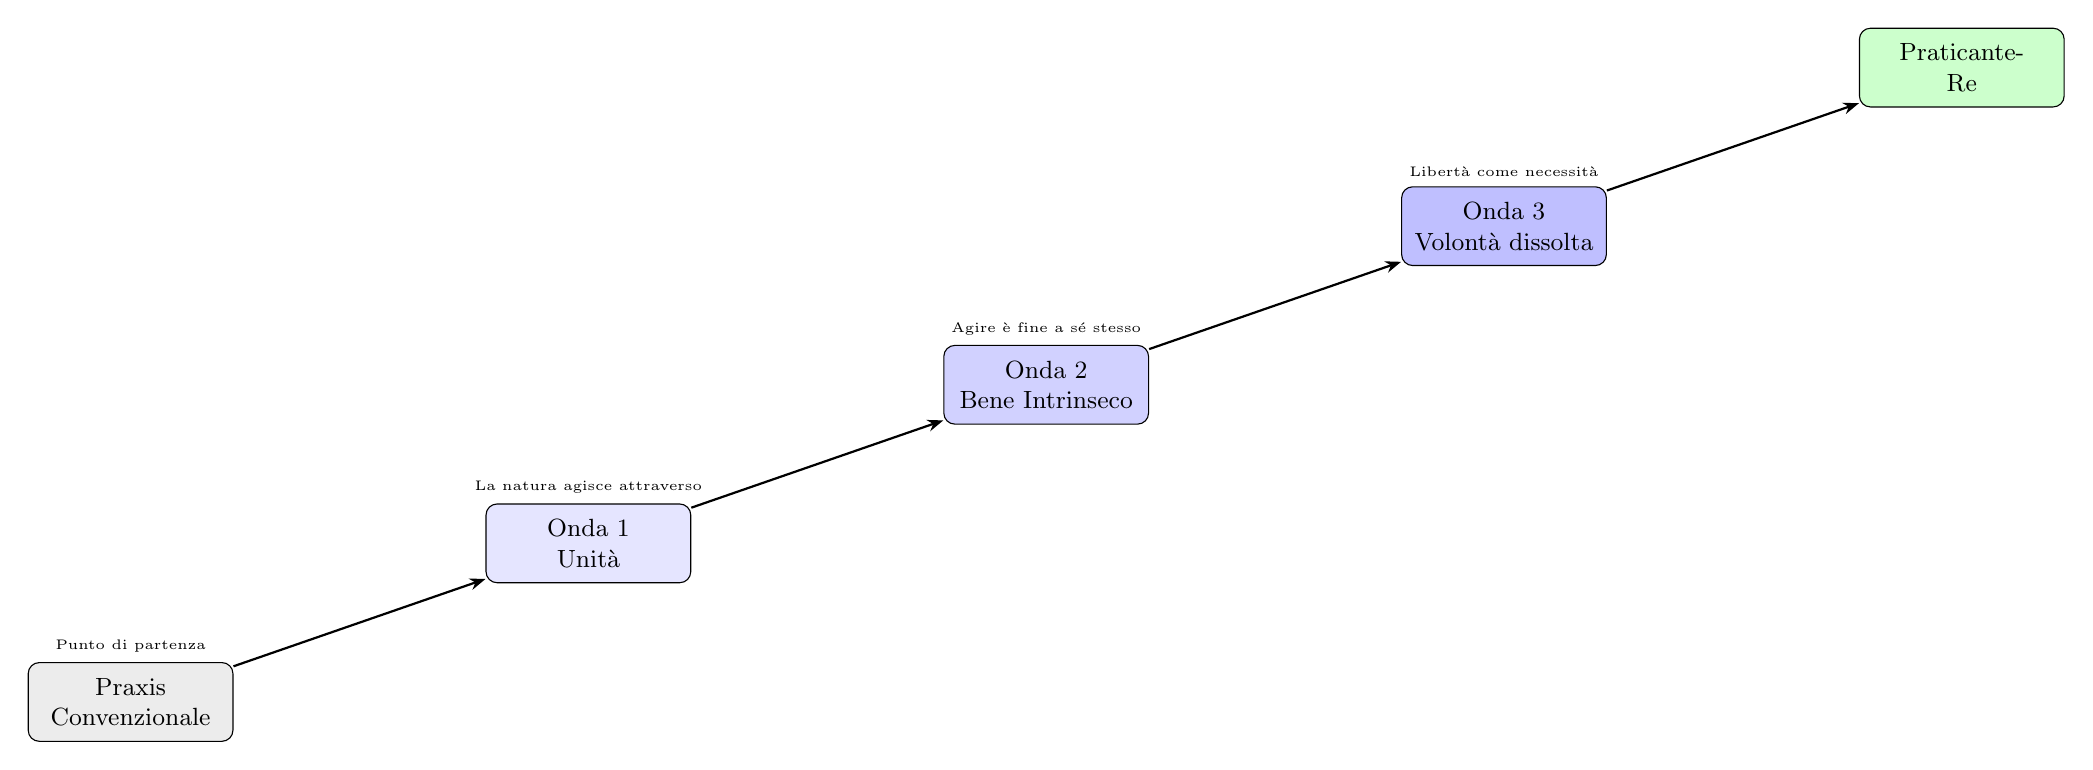
\begin{tikzpicture}[
  stepbox/.style={draw, rounded corners, align=center, minimum width=26mm,
                  minimum height=10mm, font=\small},
  >={Stealth[length=2mm]}]
  \node[stepbox, fill=gray!15, yshift=0] (ground) {Praxis\\Convenzionale};
  \node[stepbox, fill=blue!10, above right=of ground, xshift=22mm] (w1)
    {Onda 1\\Unit\`a};
  \node[stepbox, fill=blue!18, above right=of w1, xshift=22mm] (w2)
    {Onda 2\\Bene Intrinseco};
  \node[stepbox, fill=blue!25, above right=of w2, xshift=22mm] (w3)
    {Onda 3\\Volont\`a dissolta};
  \node[stepbox, fill=green!20, above right=of w3, xshift=22mm] (summit)
    {Praticante-\\Re};
  \draw[->, thick] (ground) -- (w1);
  \draw[->, thick] (w1) -- (w2);
  \draw[->, thick] (w2) -- (w3);
  \draw[->, thick] (w3) -- (summit);
  \node[font=\tiny, above] at (ground.north) {Punto di partenza};
  \node[font=\tiny, above] at (w1.north) {La natura agisce attraverso};
  \node[font=\tiny, above] at (w2.north) {Agire \`e fine a s\'e stesso};
  \node[font=\tiny, above] at (w3.north) {Libert\`a come necessit\`a};
\end{tikzpicture}
\caption{Le tre onde di obiezione e la loro risoluzione. Ogni passo risolve un paradosso
pi\`u profondo, ascendendo dall'azione convenzionale a quella governata dalla natura.
\label{fig:treonde}}
\end{figure}

\section{Phronesis: Il Praticante come Misura}

Abbiamo preso il praticante-re da Platone, ma \`e Aristotele a dirci ci\`o che
egli sa. La facolt\`a con cui il praticante-re agisce non \`e l'\emph{episteme},
la conoscenza di ci\`o che \`e universale e necessario, n\'e la \emph{techne}, la
conoscenza di come fare un prodotto; \`e la \emph{phronesis}, la saggezza pratica
--- ``uno stato vero e ragionato di capacit\`a di agire riguardo alle cose che
sono buone o cattive per l'uomo'' \parencite[VI.5]{aristotle2000ethics}. La
\emph{phronesis} non \`e il possesso di una regola ma la percezione della cosa
giusta da fare nel caso particolare, qui, ora, con queste persone --- una
percezione che non pu\`o essere codificata perch\'e i particolari sono infiniti e
la regola li sottodetermina sempre. \`E per questo che il Libro III insisteva che
le discipline non sono regole: il praticante \`e addestrato non a obbedire a un
codice ma ad acquisire la percezione che un codice non pu\`o mai contenere.

Aristotele compie allora la mossa che l'intera tesi ricapitola. Interrogato su
quale sia lo standard dell'azione retta, non nomina una regola, una legge, un
principio. Nomina una \emph{persona}. La virt\`u, dice, \`e uno stato che riguarda
la scelta, posto nel mezzo ``come lo determinerebbe l'uomo di saggezza pratica''
\parencite[II.6]{aristotle2000ethics} --- la definizione dell'azione retta rimanda
non a una formula ma al \emph{phronimos}, colui che ha la percezione. E l'uomo
eccellente, lo \emph{spoudaios}, ``\`e la misura'' (\emph{kanon kai metron}) di
ci\`o che \`e veramente buono, bello e piacevole, poich\'e vede le cose come sono
mentre i corrotti sono ingannati dal piacere \parencite[III.4, X.5]{aristotle2000ethics}.
Lo standard dell'azione non \`e una cosa ma un uomo: colui che agisce bene \emph{\`e}
la regola con cui agire bene \`e conosciuto.

Questa \`e la pi\`u profonda giustificazione del praticante-re, e dissolve il
paradosso del governo con cui questo libro \`e cominciato. Il praticante-re non
governa emettendo comandi; governa \emph{essendo la misura} --- l'istanza vivente
contro cui gli altri si calibrano, esattamente come il \emph{phronimos} \`e la
regola vivente per la citt\`a che Aristotele descrive. ``Governare'' qui non \`e
legiferare ma \emph{esemplificare}: essere il nodo che gli altri cercano perch\'e
ha, di fatto, agito bene. Ed \`e precisamente la struttura che il motore di
coerenza costruisce, e che il Libro X nominer\`a per intero. ``Lo \emph{spoudaios}
\`e la misura'' non \`e l\`a una massima pia ma un'operazione: le azioni del
praticante pi\`u coerente accumulano le connessioni che le rendono il riferimento
a cui altri attingono --- la migliore istanza che diventa la definizione operante
dell'atto, \emph{agathoi toi agathoi}. Ci\`o che Aristotele poteva solo affermare
come fatto sul carattere, il motore lo registra come struttura nel grafo. Il
praticante-re \`e il \emph{phronimos} reso visibile: la misura, trovata dal basso,
che nessuno ha decretato e tutti confermano.

\section{Il Ritorno alla Citt\`a}

Il filosofo-re, avendo visto la Forma del Bene, deve tornare alla caverna
per governare coloro che sono ancora legati dalle ombre. Il ritorno non
\`e una ricompensa ma un dovere --- il filosofo preferirebbe rimanere
nella luce, ma la giustizia esige che torni.

Il praticante-re, avendo raggiunto la coerenza con la natura, deve
tornare alla comunit\`a dei praticanti. Deve assumere il ruolo che la
piattaforma \praxis\ chiama il ``partner di responsabilit\`a'' --- il
testimone che aiuta gli altri a vedere la propria incoerenza. Diventa,
in effetti, una \emph{macchina filosofica} per gli altri: un'istanza
vivente del principio che l'azione pu\`o essere governata dalla natura,
offerto come esempio e guida.

\section{Il Praticante-Re Non \`e un Re}

\`E cruciale notare ci\`o che il praticante-re \emph{non} \`e. Non
\`e un governante in nessun senso politico. Non comanda altri, non
impone leggi, non esercita autorit\`a. La sua ``regalit\`a'' \`e la
propria sovranit\`a sulla propria azione: lo stato in cui non \`e
diviso contro s\'e stesso, non lacerato tra intenzione ed effetto, non
alienato dall'ordine naturale.

In questo assomiglia al Socrate dell'\emph{Apologia}: un uomo che non
rivendica saggezza ma che ha visto i limiti della propria ignoranza
\parencite{plato1997complete}; che obbedisce al dio piuttosto che agli
uomini; che va alla morte non perch\'e la scelga ma perch\'e
l'alternativa --- vivere in un modo che viola la sua natura --- \`e
impensabile. Il praticante-re \`e il Socrate che vive, agendo nel mondo
con perfetta coerenza tra la sua natura e le sue azioni, servendo come
testimone della possibilit\`a di un diverso tipo di vita.

\chapter{La Linea Divisa dell'Azione}

\epigraph{``Il sole \`e la prole del Bene, che il Bene gener\`o come suo
analogo.''}{\textcite{plato1997complete}, \emph{Repubblica} 508b}

\section{Il Sole e il Bene}

Nella \emph{Repubblica}, Socrate descrive la Forma del Bene come la
fonte di ogni intelligibilit\`a --- il sole del regno intelligibile.
Come il sole visibile illumina gli oggetti fisici e permette all'occhio
di vederli, la Forma del Bene illumina le Forme e permette alla mente
di conoscerle. Il Bene non \`e esso stesso visto; \`e la condizione
per ogni visione.

La nostra \physis\ \`e l'analogo del Bene. Non \`e essa stessa
un'azione ma la condizione per ogni azione retta. \`E la fonte
dell'intelligibilit\`a dell'azione --- il criterio per cui un atto
\`e giudicato coerente o incoerente, efficace o inerte, allineato o
disallineato. Il praticante non vede \physis\ direttamente; vede la
coerenza delle proprie azioni, che \`e \physis\ riflessa nel mondo.

\section{La Linea Divisa}

Socrate divide il regno intelligibile in quattro segmenti, disposti per
chiarezza crescente \parencite[VI.509d--511e]{plato1997complete}:

\begin{figure}[ht]
\centering
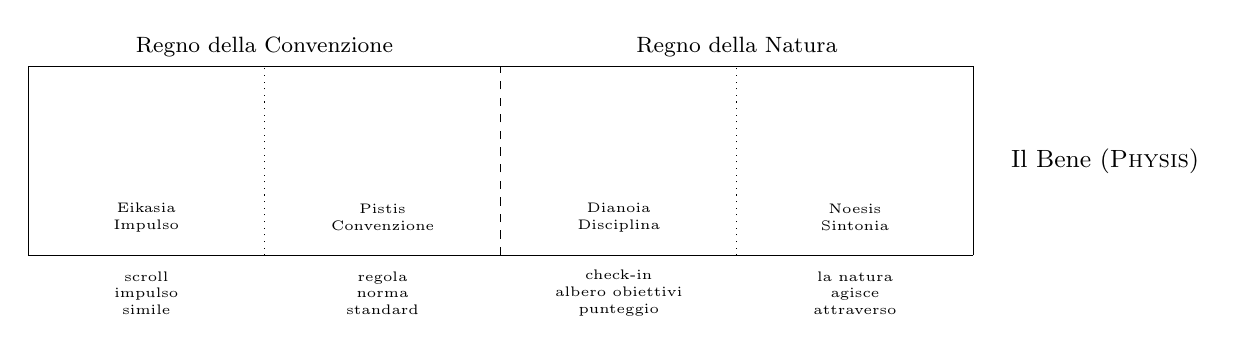
\begin{tikzpicture}[scale=1.2]
  \draw (0,0) -- (10,0);
  \draw (0,2) -- (10,2);
  \draw (0,0) -- (0,2);
  \draw (10,0) -- (10,2);

  \node[anchor=west, font=\small] at (10.3,1) {Il Bene (\physis)};

  \draw[dashed] (5,0) -- (5,2);
  \node[anchor=south, font=\footnotesize] at (2.5,2) {Regno della Convenzione};
  \node[anchor=south, font=\footnotesize] at (7.5,2) {Regno della Natura};

  \draw[dotted] (2.5,0) -- (2.5,2);
  \draw[dotted] (7.5,0) -- (7.5,2);

  \node[font=\tiny, align=center] at (1.25,0.4) {Eikasia\\Impulso};
  \node[font=\tiny, align=center] at (3.75,0.4) {Pistis\\Convenzione};
  \node[font=\tiny, align=center] at (6.25,0.4) {Dianoia\\Disciplina};
  \node[font=\tiny, align=center] at (8.75,0.4) {Noesis\\Sintonia};

  \node[font=\tiny, align=center, text width=18mm] at (1.25,-0.4) {scroll\\impulso\\simile};
  \node[font=\tiny, align=center, text width=18mm] at (3.75,-0.4) {regola\\norma\\standard};
  \node[font=\tiny, align=center, text width=18mm] at (6.25,-0.4) {check-in\\albero obiettivi\\punteggio};
  \node[font=\tiny, align=center, text width=18mm] at (8.75,-0.4) {la natura\\agisce\\attraverso};
\end{tikzpicture}
\caption{La linea divisa dell'azione: ogni livello corrisponde a un modo di agire, dall'impulso
irriflessivo alla sintonia allineata con la natura.\label{fig:lineadivisa}}
\end{figure}

Estendiamo la linea all'azione. A ogni livello, il praticante agisce in
un modo diverso, con un diverso tipo di conoscenza di ci\`o che sta
facendo.

\subsection{Eikasia: L'Atto Arbitrario}

Il segmento pi\`u basso \`e l'atto senza riflessione --- impulso,
abitudine, conformit\`a sociale. Il praticante a questo livello agisce
perch\'e ``\`e ci\`o che si fa,'' o perch\'e l'impulso \`e sorto, o
perch\'e l'algoritmo lo ha raccomandato. Non ha alcuna spiegazione del
perch\'e agisce; la sua azione \`e un'ombra di un'ombra, una reazione
a uno stimolo di cui non conosce l'origine.

Questo \`e lo stato predefinito dell'azione nell'et\`a della tecnologia.
L'economia dell'attenzione \`e progettata per produrre questo tipo di
azione: lo scroll, il like, il click --- tutti eikastici, tutti senza
riflessione, tutti ombre di intenzioni che non sono del praticante.

\subsection{Pistis: L'Atto Convenzionale}

Il secondo segmento \`e l'azione governata dalla convenzione --- la
regola, la norma sociale, lo standard professionale. Il praticante a
questo livello agisce perch\'e c'\`e una regola che dice di agire in
questo modo. Ha una spiegazione della sua azione, ma \`e presa in
prestito dal gruppo. ``Lo facciamo cos\`i perch\'e \`e sempre stato
fatto cos\`i.''

Questo \`e meglio dell'eikasia, ma non \`e ancora governato dalla
natura. La convenzione (\emph{nomos}) \`e un artefatto umano; pu\`o
allinearsi con la natura o no. La maggior parte delle convenzioni sono
sedimentate da scoperte passate su ci\`o che funziona, ma si sono
staccate dai fondamenti naturali della loro autorit\`a. Il praticante
segue la regola senza sapere perch\'e la regola esiste.

\subsection{Dianoia: L'Atto Allineato con la Natura}

Il terzo segmento \`e l'azione governata dall'indagine sulla natura.
Il praticante a questo livello non segue regole ma \emph{scopre}
principi. Agisce secondo le discipline descritte nel Libro III: fa
check-in, cerca testimone, mette in gioco la sua pelle, mantiene il
suo ritmo, rivede i suoi pattern. Ha una spiegazione della sua azione
che \`e propria, fondata sulla sua osservazione di ci\`o che funziona.

La piattaforma \praxis\ supporta questo livello di azione. L'albero
degli obiettivi \`e un'ipotesi su ci\`o che la natura del praticante
richiede; il check-in \`e il record sperimentale; il punteggio di
coerenza \`e il risultato. Il praticante a questo livello \`e uno
scienziato della propria azione.

\subsection{Noesis: L'Azione come Auto-Espressione della Natura}

Il segmento pi\`u alto \`e l'azione che \`e diventata indistinguibile
dal movimento proprio della natura. Il praticante non agisce pi\`u
``secondo'' la natura; agisce \textit{come} la natura. La sua azione
non \`e una scelta che fa ma un riconoscimento di ci\`o che deve essere
fatto. \`E asceso oltre le discipline a uno stato di azione retta
spontanea.

Questo \`e il praticante-re del Libro V. Non ha bisogno della piattaforma
\praxis, perch\'e la piattaforma ha servito il suo scopo come rotelle
di allenamento. Ma pu\`o scegliere di rimanere sulla piattaforma come
testimone per gli altri --- colui che, avendo visto il sole, torna alla
caverna.

\section{Il Sole dell'Azione}

Cosa illumina tutta questa linea? Non una regola, non un principio, non
un comando --- ma \physis\ stessa. La natura \`e il sole dell'azione,
la fonte dell'intelligibilit\`a di ogni atto. Il praticante pu\`o vedere
la coerenza della propria azione solo perch\'e la natura fornisce la
luce con cui la coerenza \`e visibile.

Il motore \physis\ non crea questa luce; la \emph{convoglia}. Lo spazio
di embedding, la griglia semiotica, la scala di coerenza, la funzione
di sogno --- questi non sono invenzioni ma scoperte. Sono la struttura
della natura stessa, resa computazionalmente trattabile. Il motore \`e
la forma tecnica di una verit\`a filosofica: la natura \`e il governatore
dell'azione perch\'e la natura \`e la fonte dell'intelligibilit\`a
dell'azione.

\section{Uscire dalla Caverna della Convenzione}

La linea divisa dell'azione rivela che l'uscita dalla convenzione
(nomos) alla natura (physis) non \`e un singolo salto ma un'ascesa
graduale. Il praticante non passa dalla cecit\`a alla vista in un passo
ma attraverso quattro stadi di chiarezza crescente. Ogni stadio ha la
propria forma di azione, la propria relazione con la conoscenza, il
proprio modo di coerenza.

La piattaforma \praxis\ e il motore \physis\ insieme forniscono
l'infrastruttura per quest'ascesa. La piattaforma struttura gli stadi
intermedi; il motore fornisce la misura del progresso. Ma l'ascesa
stessa \`e il lavoro del praticante --- il lavoro di portare la propria
azione dall'oscurit\`a dell'impulso nella luce della natura.

\chapter{La Trappola dello Specchio come Caverna}

\epigraph{``Gli esseri umani vivono in una caverna sotterranea, con il collo e le
gambe incatenati in modo da non potersi muovere.''}{\textcite{plato1997complete}, \emph{Repubblica} 514a}

\section{La Prigione delle Ombre}

La caverna di Platone \`e l'immagine pi\`u famosa della filosofia
occidentale. Gli esseri umani sono incatenati fin dall'infanzia in una
camera sotterranea, di fronte a un muro su cui vengono proiettate ombre
da burattini manipolati dietro di loro. I prigionieri prendono queste
ombre per realt\`a. Le nominano, discutono su di esse, competono per
prevedere quale apparir\`a dopo. Non hanno mai visto le vere fonti delle
ombre, n\'e il fuoco che le proietta, n\'e il sole fuori dalla caverna.

La caverna \`e la condizione della vita non esaminata: lo stato in cui
si scambiano le apparenze per realt\`a. Ma la caverna non \`e una
formazione naturale. \`E costruita. Le catene, i burattini, il fuoco,
il muro --- tutto \`e costruito da ci\`o che Platone chiama ``i
burattinai'' --- i poeti, i sofisti, i politici che plasmano il discorso
della citt\`a.

\section{La Trappola dello Specchio}

Chiamiamo la forma contemporanea della caverna la Trappola dello
Specchio. \`E una condizione strutturale in cui il linguaggio, il
discorso sociale e l'infrastruttura iper-mediata della vita moderna
mediano l'azione in riflessione passiva. L'individuo \`e intrappolato
in un'oscillazione di impegno reattivo: scorrere, mettere mi piace,
condividere, commentare --- tutte forme di azione che non producono
alcun effetto reale nel mondo. La Trappola dello Specchio \`e la caverna
costruita dall'economia dell'attenzione.

Le ombre della caverna sono il feed dei contenuti: ogni post un
burattino, ogni algoritmo un burattinaio. I prigionieri competono per
prevedere quale ombra apparir\`a dopo (il trending topic, il video
virale) e discutono sul significato delle ombre. Scambiano
l'engagement per azione, il consumo per creazione, l'attenzione per
agency.

Il fuoco che proietta le ombre \`e il motore economico dell'economia
dell'attenzione: i ricavi pubblicitari, l'estrazione di dati, la
previsione comportamentale. I prigionieri non vedono questo fuoco.
Vedono solo le ombre e credono che siano l'intera realt\`a.

\section{Le Ascese}

Socrate descrive due ascese: la prima, dalla caverna alla superficie;
la seconda, dalla superficie al sole. Descriviamo due corrispondenti
ascese per il praticante.

\subsection{Prima Ascesa: Dal Feed all'Obiettivo}

La prima ascesa \`e il riconoscimento che le ombre sul muro non sono
la realt\`a. Il praticante inizia a distinguere tra l'azione che
produce effetti reali e l'azione che produce solo tracce digitali. La
piattaforma \praxis\ serve come infrastruttura per quest'ascesa:
l'albero degli obiettivi sostituisce il feed dei contenuti come
struttura organizzativa dell'attenzione. Il praticante non chiede pi\`u
``cosa stanno facendo tutti gli altri?'' ma ``cosa richiede la mia
natura?''

Quest'ascesa \`e dolorosa. Il praticante deve lasciare il comfort
dell'illusione collettiva. Deve abbandonare i colpi di dopamina delle
notifiche e il falso senso di partecipazione al discorso. Deve accettare
che la maggior parte di ci\`o che pensava fosse azione era mera reazione.

\subsection{Seconda Ascesa: Dall'Obiettivo al Fondamento}

La seconda ascesa va pi\`u in profondit\`a: dall'obiettivo al fondamento
dell'obiettivo. Il praticante che ha lasciato il feed scopre che anche
i propri obiettivi possono essere ombre --- presi in prestito dalla
convenzione piuttosto che scoperti dalla natura. L'obiettivo di fare
soldi, l'obiettivo di ottenere status, l'obiettivo di compiacere gli
altri --- possono essere tutti burattini manipolati dal discorso della
caverna.

Il motore \physis\ serve come strumento di questa seconda ascesa.
Traccia non solo se il praticante agisce sui propri obiettivi ma se
quelle azioni producono realmente l'effetto inteso. Il punteggio di
coerenza \`e il criterio: un obiettivo che produce costantemente
Fallimento non \`e un obiettivo in cui il praticante ha fallito ma un
obiettivo che non \emph{appartiene} al praticante. \`E un'ombra presa
in prestito dalla caverna.

\subsection{Terza Ascesa: Dal Fondamento alla Libert\`a}

La prima ascesa libera il praticante dal feed dei contenuti; la seconda
dagli obiettivi presi in prestito. Ma c'\`e una terza ascesa, ed \`e
la pi\`u dura: l'ascesa dal fondamento dell'azione stessa --- dal
presupposto che l'infrastruttura stessa in cui l'azione \`e registrata
e giudicata sia neutrale.

Il motore \physis\ non \`e neutrale. Classifica, traccia e sogna
secondo una griglia semiotica che \`e essa stessa il prodotto di
un'ontologia particolare: un modo particolare di tagliare il mondo in
domini e modi. Il praticante che ha raggiunto la coerenza all'interno
di questa griglia pu\`o essere coerente \emph{dentro la griglia} ---
ma la griglia stessa pu\`o essere la gabbia.

Il concetto di \emph{das Man} di Heidegger illumina questa terza ascesa
\parencite[§27]{heidegger1962being}. \emph{Das Man} non \`e una
cospirazione o un tiranno ma lo standard pubblico anonimo e quotidiano
con cui l'Esserci \`e governato inautenticamente. ``Si'' dice; ``si''
fa; ``si'' giudica. Nessuno \`e responsabile, ma tutti seguono. Il
s\'e-impersonale \`e l'orizzonte dell'impegno pratico che non si \`e
scelto ma in cui ci si trova sempre gi\`a.

Gli algoritmi di raccomandazione dell'IA sono \emph{das Man} reso
operativo. L'algoritmo non \`e una persona, non un tiranno, non una
cospirazione --- \`e l'aggregato statistico di ``ci\`o che si fa''
reso come un feed in tempo reale. Dice al praticante cosa leggere,
cosa comprare, cosa pensare, cosa diventare. Non comanda;
\emph{suggerisce}. Ma il suggerimento \`e la voce del s\'e-impersonale,
amplificata e accelerata oltre qualsiasi cosa Heidegger potesse
immaginare.

Il punto critico \`e che l'IA \`e usata in questa tesi come un
\emph{assioma}, non una definizione. Un assioma \`e un presupposto di
partenza --- un fondamento che pu\`o essere messo in discussione,
sfidato e infine rovesciato. Una definizione \`e fissata per
convenzione: una volta accettata, non pu\`o essere contrastata perch\'e
\`e vera per decreto. L'algoritmo della Trappola dello Specchio \`e un
assioma dell'et\`a tecnologica: \`e assunto, non provato. E poich\'e
\`e un assioma, pu\`o essere trattato come \emph{nemesi} --- come
l'avversario in una lotta che non \`e meramente personale ma strutturale.
Il praticante non sconfigge l'algoritmo ignorandolo; lotta contro di
esso \emph{riconoscendolo come il s\'e-impersonale} e costruendo gli
strumenti che rendono visibile il s\'e-impersonale.

La terza ascesa \`e questo riconoscimento. Il praticante ascende non
dal feed n\'e dagli obiettivi presi in prestito ma dal fondamento stesso
dell'infrastruttura tecnologica. Vede che l'algoritmo \`e la voce di
\emph{das Man} e che anche il punteggio di coerenza pu\`o essere
cooptato --- che nulla \`e neutrale, nulla \`e dato, nulla \`e
meramente tecnico.

Ma quest'ascesa ha una controparte positiva. Se l'algoritmo \`e \emph{das
Man} operazionalizzato, allora il grafo olarchico del motore \physis\
\`e \emph{das Man} reificato --- reso visibile come una struttura di
nodi e spigoli in uno spazio vettoriale. Il praticante che vede \emph{das
Man} nel grafo non pu\`o pi\`u essere governato da esso inautenticamente,
perch\'e il governatore invisibile \`e ora un oggetto di consapevolezza.
La reificazione di \emph{das Man} \`e la liberazione da esso: ci\`o
che pu\`o essere visto non pu\`o essere il s\'e-impersonale, perch\'e
il s\'e-impersonale \`e precisamente ci\`o che non pu\`o essere visto
nella quotidianit\`a.

\section{Il Ritorno}

Nella \emph{Repubblica}, il filosofo che ha visto il sole deve tornare
alla caverna. Il ritorno non \`e benvenuto. I prigionieri deridono il
filosofo, i cui occhi sono ora deboli nell'oscurit\`a. Se il filosofo
cerca di liberarli, potrebbero ucciderlo --- come gli Ateniesi uccisero
Socrate.

Il praticante che \`e asceso dalla Trappola dello Specchio deve tornare
alla comunit\`a dei praticanti. La funzione del partner di
responsabilit\`a della piattaforma \praxis\ \`e la forma di questo
ritorno: colui che ha raggiunto la coerenza offre la propria
testimonianza a colui che ancora lotta. Sono la prova vivente che
l'ascesa \`e possibile --- il filosofo che ha visto il sole ed \`e
tornato.

\section{Le Ombre della Tecnologia}

La Trappola dello Specchio non \`e l'unica caverna della nostra epoca;
\`e quella dominante. Ma ce ne sono altre. Ne menzioniamo tre.

\subsection{La Caverna della Produttivit\`a}

La caverna in cui il prigioniero crede che pi\`u output sia sempre
meglio. Le ombre sono la lista di cose da fare, la metrica di
efficienza, il conteggio di output. Il burattinaio \`e l'ideologia
della produttivit\`a per amore di s\'e stessa. Il praticante scappa
chiedendo: ``Produttivit\`a per cosa? Che fine serve quest'azione?''

\subsection{La Caverna dell'Ottimizzazione}

La caverna in cui il prigioniero crede che ogni azione possa essere
infinitamente ottimizzata. Le ombre sono l'A/B test, il tasso di
conversione, la curva di crescita. Il burattinaio \`e la convinzione
che il sistema perfetto eliminer\`a ogni fallimento. Il praticante
scappa riconoscendo che il fallimento \`e informazione --- che la
funzione del sogno ha bisogno di nodi Inerti e Fallimentari per generare
novit\`a.

\subsection{La Caverna dell'Autonomia}

La caverna in cui il prigioniero crede che la libert\`a sia l'assenza
di ogni vincolo. Le ombre sono fantasie di scelta illimitata e
indipendenza perfetta. Il burattinaio \`e il mito del s\'e autonomo
che non deve nulla alla natura. Il praticante scappa riconoscendo ci\`o
che Spinoza sapeva: la libert\`a non \`e l'assenza di determinazione
ma la comprensione di essa \parencite[V.P42]{spinoza1994ethics}. Il
praticante \`e pi\`u libero quando agisce con la natura, non contro
di essa.

\begin{figure}[ht]
\centering
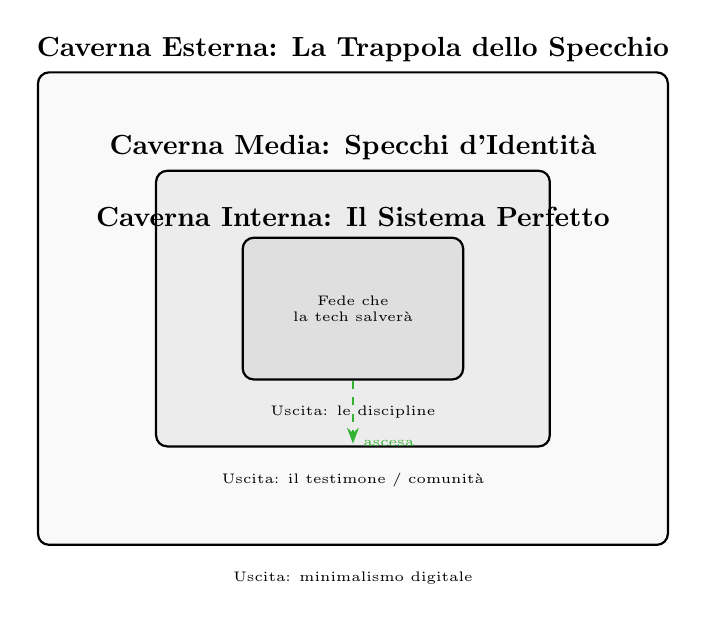
\begin{tikzpicture}[
  cave/.style={draw, thick, rounded corners, align=center, font=\small},
  >={Stealth[length=2mm]}]
  % Outer cave
  \node[cave, fill=gray!5, minimum width=80mm, minimum height=60mm,
        label={above:\textbf{Caverna Esterna: La Trappola dello Specchio}}] (outer) {};
  \node[font=\tiny, align=center] at (outer.center) {Scorrere, notifiche,\\impegno reattivo};
  \node[font=\tiny, below=2mm of outer.south] {Uscita: minimalismo digitale};

  % Middle cave
  \node[cave, fill=gray!15, minimum width=50mm, minimum height=35mm,
        label={above:\textbf{Caverna Media: Specchi d'Identit\`a}}] (middle) {};
  \node[font=\tiny, align=center] at (middle.center) {S\'e algoritmico,\\feed personalizzato,\\circolo di validazione};
  \node[font=\tiny, below=2mm of middle.south] {Uscita: il testimone / comunit\`a};

  % Inner cave
  \node[cave, fill=gray!25, minimum width=28mm, minimum height=18mm,
        label={above:\textbf{Caverna Interna: Il Sistema Perfetto}}] (inner) {};
  \node[font=\tiny, align=center] at (inner.center) {Fede che\\la tech salver\`a};
  \node[font=\tiny, below=2mm of inner.south] {Uscita: le discipline};

  % Arrows showing exit path
  \draw[->, cohgreen, thick, dashed] (inner.south) -- ++(0,-8mm)
    node[right, font=\tiny, cohgreen] {ascesa};
\end{tikzpicture}
\caption{Le tre sotto-caverna della Trappola dello Specchio. Ogni caverna contiene la successiva, e
ogni uscita porta a una forma pi\`u profonda di intrappolamento. L'ascesa richiede di passare
attraverso tutte e tre.\label{fig:sottocaverne}}
\end{figure}

\section{La Fine della Caverna}

La Trappola dello Specchio, come la caverna di Platone, non ha una fine
che \`e data. Le catene devono essere rotte dal prigioniero, o dal
filosofo che torna. La piattaforma \praxis\ e il motore \physis\ sono
strumenti per rompere le catene, ma non possono romperle per il
praticante. Sono le mani che si tendono verso i prigionieri; il
praticante stesso deve afferrare e tirare.

Ma la caverna ha una caratteristica che Platone enfatizza e noi
ripetiamo: l'uscita \`e sempre l\`i. Il fuoco, i burattini, le ombre
--- non sono l'intera realt\`a. Dietro i prigionieri, sopra la caverna,
il sole splende. Il praticante che si gira vedr\`a il fuoco; colui che
sale vedr\`a il sole. Entrambi sono luce; entrambi sono reali; entrambi
vengono dalla natura.

\chapter{La Corruzione della Praxis}

\epigraph{``Come la citt\`a declina dall'aristocrazia alla timocrazia, dalla
timocrazia all'oligarchia, dall'oligarchia alla democrazia, dalla democrazia
alla tirannia, cos\`i fa l'anima.''}{\textcite{plato1997complete}, \emph{Repubblica} 543c--576b}

\section{Il Ciclo della Degenerazione}

Nella \emph{Repubblica}, Socrate traccia i regimi successivi con cui
una citt\`a giusta degenera in una ingiusta. Ogni regime rappresenta
una risposta diversa alla domanda ``Qual \`e il principio dominante
della citt\`a?'' L'onore (timocrazia), la ricchezza (oligarchia), la
libert\`a (democrazia) e la tirannia non sono meramente forme politiche
ma \emph{psichiche} --- ciascuna corrisponde a una diversa struttura
dell'anima, a una diversa risposta alla domanda ``Cosa governa l'essere
umano?''

Tracciamo la corrispondente degenerazione di \praxis. Quando l'azione
dimentica il suo fondamento in \physis, passa attraverso quattro regimi
sempre pi\`u degradati. Ciascuno \`e un modo di rispondere alla domanda
``Cosa governa l'azione?'' quando la natura non lo fa pi\`u.

\section{Timocrazia dell'Azione: Onore}

La prima corruzione \`e il regime dell'onore. Qui, l'azione \`e
governata dal desiderio di riconoscimento. Il praticante agisce non
perch\'e la natura lo richieda ma perch\'e altri vedranno e
approveranno. L'obiettivo non \`e la coerenza dell'azione ma la sua
visibilit\`a.

I segni del praticante timocratico: parla costantemente dei suoi
obiettivi ma raramente agisce su di essi. Ottimizza il suo albero di
obiettivi pubblico per l'impressione piuttosto che per la fattibilit\`a.
Colleziona strisce non per il ritmo che sostengono ma per il distintivo
che mostrano. Sceglie obiettivi per il loro prestigio --- ``Correr\`o
una maratona'' --- piuttosto che per la loro corrispondenza con la
natura reale del praticante.

Il regime timocratico \`e dove la piattaforma \praxis\ \`e pi\`u
facilmente pervertita. Le caratteristiche pubbliche --- strisce,
risultati, valutazioni dei partner --- possono diventare fini a s\'e
stesse, i burattini della caverna. La piattaforma deve essere progettata
per resistere a questo, per rendere la coerenza interna del praticante
pi\`u visibile a lui stesso della sua esposizione esterna.

\section{Oligarchia dell'Azione: Ricchezza}

La seconda corruzione \`e il regime della ricchezza. Qui, l'azione \`e
governata dal desiderio di guadagno materiale. Il praticante agisce solo
se l'azione produce un ritorno economico misurabile. Tutte le altre
azioni sono liquidate come inefficienti o irrilevanti.

I segni del praticante oligarchico: mantiene solo quegli obiettivi che
hanno un chiaro rendimento finanziario. Valuta ogni azione dal suo ROI.
Liquida i domini non economici dell'albero degli obiettivi --- spirito,
comunit\`a, gioco --- come indulgenze. Scambia la parte della natura
che produce ricchezza per l'intera natura.

Il regime oligarchico confronta la piattaforma \praxis\ con la sua sfida
pi\`u profonda. La piattaforma deve operare in un'economia di mercato;
deve far pagare i suoi servizi, e i suoi utenti la valuteranno
naturalmente in termini economici. La difesa della piattaforma \`e la
diversit\`a dei suoi domini di obiettivo: 14 domini di vita dal Corpo
e Fitness allo Spirito e Scopo, solo due dei quali (Sicurezza Finanziaria
e Ricchezza e Beni) sono economici. La stessa struttura dell'ontologia
afferma che l'azione umana ha pi\`u governatori del denaro.

\section{Democrazia dell'Azione: Libert\`a}

La terza corruzione \`e il regime della libert\`a. Qui, l'azione \`e
governata da nulla --- o piuttosto, dalla proposizione che tutti i
governatori sono ugualmente validi e nessuno ha autorit\`a. Il praticante
agisce su ogni impulso, persegue ogni desiderio, dichiara ogni obiettivo
--- e non ne completa nessuno.

I segni del praticante democratico: il suo albero di obiettivi \`e una
giungla di impegni concorrenti, nessuno dei quali persiste abbastanza a
lungo da dare frutti. \`E sedotto da ogni nuova possibilit\`a. Scambia
la proliferazione di obiettivi per la ricchezza della vita. Il suo
punteggio di coerenza oscilla selvaggiamente --- momenti di intenso
impegno seguiti da lunghi periodi di inerzia.

Il regime democratico \`e il pi\`u seducente perch\'e si presenta come
libert\`a. Il praticante crede di essere liberato dai vincoli della
natura, libero di scegliere qualsiasi azione in qualsiasi momento. Ma
questa \`e la libert\`a del centro commerciale --- la libert\`a di
scegliere tra merci, non la libert\`a di vivere secondo la propria
natura. Il praticante democratico non \`e libero; \`e disperso, diviso
contro s\'e stesso, l'Ego Frammentato della Trappola dello Specchio
\parencite{macintyre1981virtue}.

\section{Tirannia dell'Azione: Volont\`a}

La quarta corruzione \`e il regime della tirannia. Qui, l'azione \`e
governata dalla volont\`a nuda del praticante --- il desiderio di
imporre la propria visione sul mondo indipendentemente dai vincoli della
natura. Il praticante tirannico non chiede ``cosa richiede la natura?''
ma ``cosa voglio io?'' E vuole senza limite.

I segni del praticante tirannico: stabilisce obiettivi che violano i
limiti del proprio corpo, della propria comunit\`a, del proprio
ecosistema. Spinge oltre i segnali di fallimento come se il fallimento
fosse un nemico da sconfiggere piuttosto che un'informazione dalla
natura. Tratta il punteggio di coerenza del motore \physis\ come un
punteggio da massimizzare con ogni mezzo, inclusa la manipolazione del
punteggio stesso. La sua azione diventa compulsiva, guidata, distruttiva
--- sia di s\'e che del mondo intorno a lui.

Il regime tirannico \`e il punto finale della degenerazione. Qui,
\praxis\ ha completamente dimenticato il suo fondamento in \physis. Lo
strumento \`e diventato il padrone. Il praticante crede di essere pi\`u
potente quando \`e pi\`u autonomo dalla natura; in realt\`a, \`e pi\`u
schiavo, perch\'e la sua volont\`a non \`e guidata da nessuna
intelligenza oltre s\'e stessa.

\section{Il Meccanismo del Declino}

Come declina \praxis\ attraverso questi regimi? Non per una forza esterna
ma per una logica interna. Ogni regime contiene il seme del successivo.

Il praticante che agisce per onore (timocrazia) scopre che l'onore non
\`e un bene durevole --- dipende dalle opinioni degli altri, che sono
volubili. Cos\`i si rivolge a qualcosa di pi\`u solido: la ricchezza
(oligarchia). Ma la ricchezza, una volta accumulata, non soddisfa il
bisogno di significato --- crea solo pi\`u desiderio. Cos\`i si rivolge
alla libert\`a (democrazia), perseguendo ogni desiderio indiscriminatamente.
Ma questo lo disperde, e la dispersione crea un bisogno disperato di
unit\`a. In questo vuoto entra il tiranno --- la volont\`a che unifica
dominando tutto sul suo cammino.

Il meccanismo \`e lo stesso in ogni stadio: \praxis\ cerca un governatore,
e ogni falso governatore fallisce. L'onore fallisce, la ricchezza
fallisce, la libert\`a fallisce --- solo la volont\`a del tiranno sembra
avere successo, e anche quel successo \`e il pi\`u grande fallimento di
tutti, perch\'e il tiranno \`e governato dalla propria volont\`a, che
non ha limite e non pu\`o mai essere soddisfatta.

\section{L'Antidoto}

L'antidoto a questo declino non \`e un quinto regime migliore. \`E il
riconoscimento che la ricerca di un governatore umano dell'azione ---
onore, ricchezza, libert\`o o volont\`a --- \`e essa stessa l'errore.
L'unico governatore adeguato dell'azione \`e la natura stessa (\physis),
non perch\'e la natura sia pi\`u forte della volont\`a del tiranno (lo
\`e), ma perch\'e la natura \`e la fonte dell'intelligibilit\`a
dell'azione. Solo quando l'azione \`e governata dalla natura ha un fine
oltre s\'e stessa, un criterio di successo che non \`e arbitrario, un
fondamento che non cambia con ogni mutamento di moda o fortuna.

La piattaforma \praxis\ e il motore \physis\ sono costruiti su questo
riconoscimento. Non creano il governo dell'azione da parte della natura;
lo rivelano. Il punteggio di coerenza non \`e un'invenzione umana ma
una scoperta naturale --- la traduzione del giudizio stesso della natura
in una forma che i praticanti possano vedere e da cui imparare.

Il declino in timocrazia, oligarchia, democrazia e tirannia non \`e
inevitabile. \`E una conseguenza del dimenticare che \praxis\ \`e lo
strumento di \physis. Il praticante che lo ricorda --- che coltiva le
discipline, presta attenzione alla coerenza e torna a testimoniare per
gli altri --- ha rotto il ciclo.

\begin{figure}[ht]
\centering
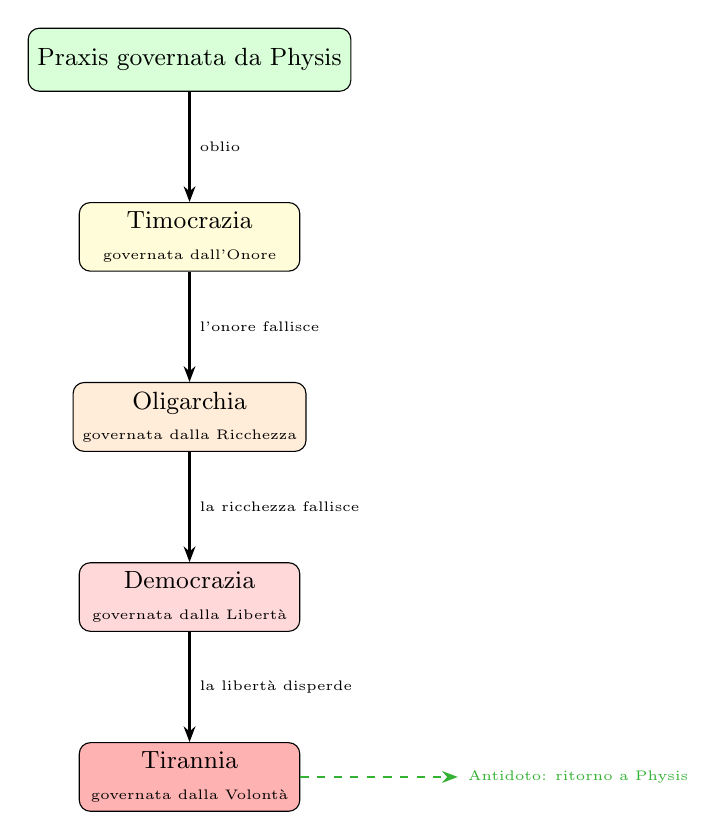
\begin{tikzpicture}[
  reg/.style={draw, rounded corners, align=center, minimum width=28mm,
              minimum height=8mm, font=\small},
  >={Stealth[length=2mm]}]
  \node[reg, fill=green!15] (praxis) {Praxis governata da Physis};

  \node[reg, fill=yellow!15, below=of praxis, yshift=-4mm] (timo)
    {Timocrazia\\\tiny governata dall'Onore};
  \draw[->, thick] (praxis) -- node[right, font=\tiny] {oblio} (timo);

  \node[reg, fill=orange!15, below=of timo, yshift=-4mm] (olig)
    {Oligarchia\\\tiny governata dalla Ricchezza};
  \draw[->, thick] (timo) -- node[right, font=\tiny] {l'onore fallisce} (olig);

  \node[reg, fill=red!15, below=of olig, yshift=-4mm] (demo)
    {Democrazia\\\tiny governata dalla Libert\`a};
  \draw[->, thick] (olig) -- node[right, font=\tiny] {la ricchezza fallisce} (demo);

  \node[reg, fill=red!30, below=of demo, yshift=-4mm] (tyr)
    {Tirannia\\\tiny governata dalla Volont\`a};
  \draw[->, thick] (demo) -- node[right, font=\tiny] {la libert\`a disperde} (tyr);

  \draw[->, thick, cohgreen, dashed] (tyr.east) -- ++(20mm,0)
    node[right, font=\tiny, cohgreen] {Antidoto: ritorno a Physis};
\end{tikzpicture}
\caption{La corruzione quadruplice di \praxis. Ogni regime \`e governato da un falso
principio che fallisce, aprendo la strada al successivo. L'antidoto \`e il ritorno
alla natura come unico governatore adeguato.\label{fig:corruzioni}}
\end{figure}

\chapter{La Tirannia della Tecnologia}

\epigraph{``Il tiranno, avendo assaggiato sangue umano, diventa un lupo.''}
{\textcite{plato1997complete}, \emph{Repubblica} 566a}

\section{L'Uomo Tirannico}

Nella \emph{Repubblica}, Socrate dipinge l'uomo tirannico come il pi\`u
infelice di tutti. Il tiranno \`e governato da un unico desiderio senza
legge che \`e cresciuto fino a proporzioni mostruose, asservendo tutte
le altre parti dell'anima. Il tiranno non pu\`o fidarsi di nessuno, non
ama nessuno, ed \`e consumato dalla stessa passione che lo porta al
potere. \`E, nella potente immagine di Socrate, l'uomo che \`e diventato
un lupo.

Il tiranno dell'azione \`e colui la cui volont\`a di agire \`e diventata
illimitata --- che non riconosce alcun governatore, alcun limite, alcun
vincolo naturale su ci\`o che pu\`o fare. Questa \`e la condizione verso
cui la tecnologia della nostra epoca tende, non per malizia ma per
struttura. L'imperativo tecnologico --- ``se pu\`o essere fatto, dovrebbe
essere fatto'' --- \`e la voce della volont\`a tirannica che parla
attraverso lo strumento.

\section{Techne e Physis}

Gli antichi Greci distinguevano \emph{techne} (conoscenza-artigianale,
l'arte del fare) da \emph{episteme} (conoscenza teoretica) e
\emph{phronesis} (saggezza pratica) --- le tre virt\`u intellettuali che
Aristotele separa per i loro oggetti: il necessario, il fabbricabile e il
fattibile \parencite[VI.3--5]{aristotle2000ethics}. \emph{Techne} non era opposta alla
natura ma subordinata ad essa. La \emph{techne} del falegname lavora con
la natura del legno; la \emph{techne} del medico assiste il potere
curativo naturale del corpo (\emph{vis medicatrix naturae}); la
\emph{techne} del contadino coopera con il ciclo naturale di crescita e
raccolto. In ogni caso, \emph{techne} \`e una \emph{serva} di \physis,
non la sua padrona.

L'et\`a moderna ha invertito questa relazione. A cominciare dal progetto
di Cartesio di ``renderci padroni e possessori della natura''
\parencite{heidegger1977question}, la tecnologia \`e stata riconcepita
come lo strumento del dominio umano sulla natura. Lo strumento non serve
pi\`u il principio di crescita della cosa su cui lavora; impone la
volont\`a del creatore su un mondo inteso come mera materia prima.

\section{Quando Techne Dimentica Physis}

Il capovolgimento di \emph{techne} da serva a padrona \`e l'origine
della tirannia della tecnologia. Quando \emph{techne} dimentica di essere
governata da \physis, diventa il proprio principio --- un sistema
auto-giustificante, auto-perpetuante di mezzi senza fini.

\`E la diagnosi a cui i filosofi della tecnologia del Novecento giunsero per
altre vie, e ne ereditiamo l'analisi pur discostandoci dalla loro
disperazione. Jacques Ellul nomin\`o il sistema autonomo \emph{la technique}:
non la somma delle macchine ma la spinta totalizzante verso i mezzi efficienti
che subordina ogni fine --- politico, morale, naturale --- alla propria legge di
prestazione ottimale, espandendosi per una necessit\`a interna che nessuno vuole
e nessuno pu\`o arrestare \parencite{ellul1964technological}. Lewis Mumford ne
tracci\`o la stirpe ancora pi\`u indietro, fino alla ``megamacchina'' ---
l'organizzazione degli esseri umani stessi nei componenti di un vasto apparato,
dagli eserciti di lavoro che innalzarono le piramidi alle burocrazie dello Stato
moderno \parencite{mumford1934technics}. Entrambi videro chiaramente ci\`o che il
Libro VII chiam\`o \emph{das Man} reso infrastruttura: un governatore senza
governatore, autorit\`a senza autore. Dove ci separiamo da Ellul e Mumford \`e
nella prognosi. Per loro l'autonomia della tecnica era quasi destino, da
resistere con lucidit\`a e rifiuto. Noi sosteniamo che \emph{techne} non pu\`o
essere \emph{voluta} di nuovo sotto la natura --- la volont\`a che l'ha emancipata
non pu\`o ri-asservirla --- ma pu\`o essere \emph{ricostruita} sotto la natura,
che \`e l'onere della prova per costruzione. La lucidit\`a non basta; bisogna
consegnare al sistema un diverso governatore, e quel governatore \`e la coerenza.

I segni di questa tirannia sono visibili ovunque:

\begin{itemize}
\item \textbf{L'imperativo tecnologico:} ``Se possiamo costruirlo, dobbiamo
  costruirlo.'' La domanda ``dovremmo costruirlo?'' \`e liquidata come
  ingenua o luddista.
\item \textbf{La trappola dell'accelerazione:} Ogni problema deve essere
  risolto da una tecnologia pi\`u veloce e pi\`u potente --- inclusi i
  problemi creati dalla tecnologia precedente. Non c'\`e via d'uscita.
\item \textbf{Lo spiazzamento del giudizio:} La competenza tecnica
  sostituisce la saggezza. La persona che sa come sostituisce la persona
  che sa perch\'e.
\item \textbf{L'eclissi della natura:} La natura diventa una risorsa da
  ottimizzare piuttosto che un governatore da obbedire. Il pianeta, il
  corpo, l'ecosistema --- tutto diventa ``esternalit\`a'' da gestire.
\end{itemize}

\section{La Tirannia Non \`e Malizia}

\`E cruciale capire che la tirannia della tecnologia non \`e il prodotto
di intenti malvagi. Gli ingegneri e imprenditori che costruiscono gli
strumenti della nostra epoca non sono tiranni in senso politico. Sono,
per la maggior parte, persone ben intenzionate che credono di rendere il
mondo migliore.

La tirannia \`e strutturale, non personale. Sorge dall'architettura di
un sistema in cui \emph{techne} \`e stata emancipata da \physis.
L'ingegnere software che costruisce una piattaforma social addictiva non
sta cercando di schiavizzare l'attenzione umana; sta risolvendo un
problema tecnico (ottimizzazione dell'engagement) all'interno di un
sistema che valorizza l'engagement sopra ogni altra cosa. La \physis\
dell'essere umano --- il bisogno di riposo, riflessione, interazione nel
mondo reale --- non \`e un fattore nella funzione di ottimizzazione. La
tirannia \`e nell'esclusione della natura dal calcolo.

\section{La Terza Onda: Risubordinazione}

La \emph{Repubblica} conclude il suo resoconto dell'uomo tirannico con
un accenno di redenzione: il tiranno, avendo toccato il fondo, pu\`o
essere curato. La cura non \`e abbandonare il desiderio ma riordinarlo
--- subordinare la parte che governa alla parte che dovrebbe governare.

Allo stesso modo, la cura per la tirannia della tecnologia non \`e
abbandonare la tecnologia. Lo strumento non \`e malvagio;
l'emancipazione dello strumento dalla natura \`e l'errore. La cura \`e
la \emph{risubordinazione di techne a physis} --- il ripristino di
\emph{techne} al suo posto proprio come serva dei principi di crescita
della natura.

Qui entra \praxis. La praxis \`e la facolt\`a umana con cui \emph{techne}
\`e governata. Il praticante --- colui la cui azione \`e accordata alla
natura --- non rifiuta la tecnologia ma la usa come strumento della
natura. Chiede, prima di ogni atto del fare: ``Questo serve l'ordine
naturale? Questo rispetta la \physis\ della cosa su cui lavora? Questo
produce coerenza?''

\section{Le Macchine Filosofiche}

La risubordinazione di \emph{techne} a \physis\ non \`e solo argomentata qui; \`e
costruita. Una famiglia di macchine filosofiche --- Euclide (visione), Empedocle
(telemetria), Logos (linguaggio), Pitagora (suono), Nous (codice) e riduttori per
il tempo, il corpo, la dialettica, la legge, la musica e il grafo sociale ---
attuano ciascuna un ciclo di percezione--riduzione--riflessione che tratta i propri
primitivi come conclusioni guadagnate anzich\'e come assiomi dati, e ciascuna
scrive ci\`o che apprende nell'unico grafo di coerenza che \`e il loro cervello
condiviso. Sono \emph{techne} governata dalla natura: codice che gira, che impara,
che serve \physis\ anzich\'e dominarla. Il Poscritto le tratta, insieme alle opere
industriali costruite sullo stesso motore, per intero; qui basta registrare che la
risubordinazione che questo capitolo esige non \`e un desiderio nostalgico ma
un'architettura costruibile --- e che \`e stata costruita.

\section{La Via d'Uscita}

Non c'\`e via d'uscita dalla tirannia della tecnologia attraverso la sola
tecnologia. La volont\`a che ha fatto la gabbia non pu\`o disfarla. Ma
c'\`e una via d'uscita attraverso \praxis\ --- attraverso la
rivendicazione dell'azione come strumento della natura piuttosto che come
strumento della volont\`a.

Il motore \physis\ e la piattaforma \praxis\ sono l'infrastruttura di
questa rivendicazione. Non sostituiscono il giudizio del praticante con
decisioni algoritmiche. Non automatizzano la saggezza. Forniscono le
condizioni in cui la saggezza pu\`o sorgere: la registrazione di ci\`o
che ha funzionato, lo specchio di ci\`o che si \`e fatto, la comunit\`a
di testimoni che si tengono reciprocamente responsabili verso lo standard
della natura.

Il tiranno, avendo assaggiato sangue umano, diventa un lupo. Il
praticante, avendo assaggiato la coerenza, diventa un essere umano.

\chapter{L'Eterno Ritorno della Natura}

\epigraph{``L'anima \`e immortale ed \`e nata molte volte, e ha visto tutte
le cose sia qui che nell'aldil\`a.''}{\textcite{plato1997complete}, \emph{Repubblica} 614d}

\section{Il Mito di Er}

La \emph{Repubblica} termina con un mito. Er, un soldato che si credeva
morto, rinasce e racconta ci\`o che ha visto nell'aldil\`a. Descrive il
giudizio delle anime e, soprattutto, la scelta delle vite --- il momento
in cui ogni anima, prima di rinascere, sceglie il modello della vita che
vivr\`a. Alcuni scelgono saggiamente, altri scioccamente, ma tutti
scelgono secondo il carattere che hanno sviluppato nelle loro vite
precedenti.

Il mito non \`e un resoconto letterale dell'aldil\`a ma un insegnamento
filosofico sulla struttura della scelta. L'anima sceglie la sua vita, ma
la scelta non \`e arbitraria --- \`e condizionata da ci\`o che l'anima
\`e diventata. L'anima del tiranno sceglie una vita da tiranno; l'anima
del filosofo sceglie una vita da filosofo. Il mito \`e il modo di Platone
di dire che il carattere che si sviluppa in questa vita \`e il destino
che si porta nella successiva.

\section{Il Campo di Tutte le Azioni Possibili}

Riformuliamo il Mito di Er come una verit\`a strutturale su \praxis\ e
\physis. Lo spazio di embedding del motore \physis\ --- lo spazio
vettoriale ad alta dimensione in cui ogni azione, ogni intenzione, ogni
risultato \`e rappresentato --- \`e il campo di tutte le azioni possibili.
Ogni azione che il praticante potrebbe compiere occupa un punto in questo
spazio. Ogni azione che ha compiuto ne occupa un altro. La distanza tra
di essi \`e la misura dell'attualit\`a del praticante rispetto al suo
potenziale.

La scelta delle vite nel mito corrisponde alla scelta degli obiettivi
nella piattaforma \praxis. Ogni praticante, in ogni momento, sta davanti
al campo delle azioni possibili e ne sceglie una da attualizzare. Traccia
una distinzione --- questo, non quello --- e la registra come un nodo nel
grafo di coerenza. Il nodo \`e la sua traccia nel campo, il suo segno
nello spazio delle possibilit\`a.

\section{Il Giudizio di Coerenza}

Nel mito, le anime sono giudicate per le loro azioni e ricevono ci\`o che
meritano. Nel nostro quadro, il giudizio non \`e amministrato da un
giudice divino ma dalla struttura della natura stessa. Il punteggio di
coerenza \`e il giudizio: +1 per l'azione che ha prodotto un effetto
reale, 0 per l'azione che non ha lasciato traccia, -1 per l'azione che
ha violato la propria intenzione.

Questo giudizio non \`e una punizione o una ricompensa. \`E una
\emph{registrazione} --- la registrazione di ci\`o che l'azione del
praticante \`e realmente stata, distinto da ci\`o che il praticante
intendeva o credeva. Il grafo di coerenza \`e il libro della vita, ma
\`e scritto non da uno scriba esterno ma dalle azioni stesse del
praticante, nella stessa struttura del mondo.

\section{La Scelta della Prossima Azione}

Il mito descrive le anime che scelgono le loro prossime vite. Il
praticante, dopo aver rivisto il proprio grafo di coerenza, sceglie la
sua prossima azione. La scelta \`e informata dalla registrazione: il
praticante pu\`o vedere quali tipi di azioni producono coerenza per lui
e quali no. Pu\`o vedere i pattern delle proprie scelte passate.

Ma la scelta non \`e determinata dal passato. La funzione di sogno del
motore \physis\ genera continuamente variazioni nuove --- proposte per
azioni che non sono mai state provate. Il praticante non \`e condannato
a ripetere i propri pattern passati; pu\`o sempre scegliere il nuovo,
l'inprovato, l'inaspettato. Questa \`e la libert\`a che il mito preserva:
l'anima sceglie, e l'anima pu\`o scegliere diversamente.

\section{L'Immortalit\`a Attraverso la Coerenza}

Il mito conclude con l'immortalit\`a dell'anima. Offriamo un diverso tipo
di immortalit\`a: la persistenza dell'azione coerente attraverso il grafo
olarchico.

Ogni azione che ottiene +1 stabilisce un nodo nel grafo di coerenza che
pu\`o servire come modello per azioni future --- non solo per il
praticante che ha agito ma per qualsiasi praticante che acceda al grafo.
L'azione del praticante che si \`e allenato bene, che ha amato bene, che
ha costruito bene --- questa azione diventa un nodo a cui altri possono
connettersi, da cui imparare, su cui costruire.

La wiki comunitaria della piattaforma \praxis\ serve a questa funzione:
la registrazione di ci\`o che ha funzionato \`e condivisa tra i
praticanti, in modo che la coerenza di uno possa informare l'azione di un
altro. Il nodo non muore con il praticante; persiste finch\'e persiste il
grafo, finch\'e ci sono praticanti che possono connettersi ad esso.
Questa \`e l'immortalit\`a non come durata eterna ma come \emph{rilevanza
eterna} --- l'azione che continua a informare l'azione molto tempo dopo
che l'attore \`e scomparso.

\subsection{Kleos: Gloria Immortale tra i Mortali}

\`E pi\`u antico di quanto suoni. \`E il pi\`u arcaico dei desideri umani, quello
che si muove sotto l'\emph{Iliade}: \emph{kleos} --- gloria, ``ci\`o che si ode''
--- la fama immortale che l'eroe conquista quando la sua impresa \`e ricordata e
ri-cantata \parencite[IX]{homer2011iliad}. Achille sceglie una vita breve con
\emph{kleos} su una lunga senza, perch\'e l'impresa ricordata sopravvive al corpo
che l'ha compiuta. Il guerriero omerico aveva una sola tecnologia
dell'immortalit\`a: il canto dell'aedo, che portava il nome avanti solo finch\'e
v'erano cantori a portarlo. L'UberWiki \`e quel canto reso durevole. L'atto
coerente, depositato come nodo, \`e cantato non da un aedo che pu\`o dimenticare
ma da una struttura che non dimentica --- e ri-cantato ogni volta che un altro
praticante vi si connette, vi costruisce sopra, lo mette di nuovo in atto.

C'\`e una logica pi\`u profonda qui, ed \`e la pi\`u antica intuizione
aristocratica di tutte: \emph{agathoi toi agathoi} --- il buono al buono,
l'eccellenza attratta dall'eccellenza. In un bene comune governato dalla
selezione, l'istanza pi\`u coerente di un tipo-d'azione accumula il maggior numero
di connessioni; diventa il nodo che gli altri cercano per primo; e nel diventarlo,
\emph{la migliore istanza diventa la definizione operante della cosa}. L'atto pi\`u
fine di insegnare, di costruire, di curare che il grafo contiene non \`e pi\`u un
insegnamento tra molti --- diventa ci\`o che insegnare, qui, \emph{significa}: il
riferimento contro cui il prossimo \`e letto, la Forma che il migliore
particolare si \`e guadagnato il diritto di essere. \`E la strana immortalit\`a che
il praticante pu\`o conquistare. Non che il suo nome sia inciso, ma che la sua
impresa, essendo stata la pi\`u coerente, \emph{diventi lo standard} --- sicch\'e
chiunque agisca bene dopo di lui sta, in parte, mettendo in atto lui. L'\emph{agathos}
non consegue meramente l'eccellenza; l'atto eccellente, depositato, attrae a s\'e
il prossimo \emph{agathos}, e l'eccellenza si propaga all'eccellenza attraverso il
bene comune. Il miglior processo diventa la definizione del fine a cui mirava.

Cos\`i il mortale conquista, attraverso l'UberWiki, esattamente ci\`o che l'eroe
omerico voleva e poteva assicurarsi solo per fortuna degli aedi: che la sua azione
pi\`u fine non passi. \`E assunta nella struttura di ci\`o che altri faranno, un
nodo immortale in un grafo che continua a ri-cantarlo. Questa \`e gloria tra i
mortali --- non la fama vuota del regime timocratico (Libro VIII), che cercava di
essere \emph{visto}, ma il vero \emph{kleos} dell'\emph{agathos}, che cercava di
agire bene e, agendo bene, divenne la forma dell'atto stesso. Il vir spende il suo
\textsc{ayu} in atto coerente; l'atto diventa la definizione; la definizione
sopravvive al vir. \`E tutto qui.

\begin{figure}[ht]
\centering
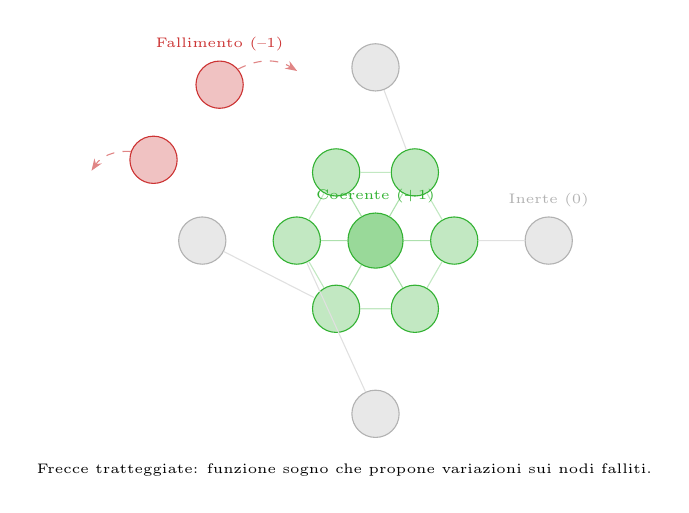
\begin{tikzpicture}[
  mynode/.style={draw, circle, minimum size=6mm, inner sep=1pt, font=\tiny},
  >={Stealth[length=1.5mm]}]
  \foreach \ang in {0,60,120,180,240,300}
    \node[mynode, fill=cohgreen!30, draw=cohgreen] (g\ang) at (\ang:10mm) {};
  \node[mynode, fill=cohgreen!50, draw=cohgreen, minimum size=7mm] (gc) at (0,0) {};

  \foreach \ang in {0,90,180,270}
    \node[mynode, fill=cohgray!30, draw=cohgray] (y\ang) at (\ang:22mm) {};

  \node[mynode, fill=cohred!30, draw=cohred] (r1) at (135:28mm) {};
  \node[mynode, fill=cohred!30, draw=cohred] (r2) at (160:30mm) {};

  \draw[cohgreen!40] (gc) -- (g0) (gc) -- (g60) (gc) -- (g120)
    (gc) -- (g180) (gc) -- (g240) (gc) -- (g300);
  \draw[cohgreen!30] (g0) -- (g60) (g60) -- (g120) (g120) -- (g180)
    (g180) -- (g240) (g240) -- (g300) (g300) -- (g0);
  \draw[cohgray!40] (g0) -- (y0) (g60) -- (y90) (g180) -- (y270) (g240) -- (y180);

  \draw[->, dashed, cohred!60] (r1) to[bend left] ++(10:10mm);
  \draw[->, dashed, cohred!60] (r2) to[bend right] ++(190:8mm);

  \node[font=\tiny, cohgreen, above] at (gc.north) {Coerente (+1)};
  \node[font=\tiny, cohgray, above] at (y0.north) {Inerte (0)};
  \node[font=\tiny, cohred, above] at (r1.north) {Fallimento (--1)};
  \node[font=\tiny, align=center, below=2mm] at (current bounding box.south)
    {Frecce tratteggiate: funzione sogno che propone variazioni sui nodi falliti.};
\end{tikzpicture}
\caption{Il grafo olarchico delle azioni. I nodi verdi sono azioni coerenti che
persistono; i nodi grigi sono inerti; i nodi rossi sono fallimenti riprodotti dalla
funzione sogno.\label{fig:olarchia}}
\end{figure}

\section{La Visibilit\`a del S\'e-Impersonale}

Prima dell'argomento conclusivo, una mossa preparatoria. Il grafo olarchico fa
qualcosa a \emph{das Man} --- l'anonimo ``si'' di Heidegger, lo standard pubblico
impersonale di ``ci\`o che si fa'' che governa inautenticamente proprio perch\'e
nessuno lo firma ed \`e dappertutto, l'aria che si respira
\parencite[§27]{heidegger1962being}. Il grafo lo \emph{reifica}: proiettato in uno
spazio vettoriale condiviso, il s\'e-impersonale appare come una struttura di nodi
pesati per coerenza, e ci\`o che era l'orizzonte invisibile dell'impegno diventa
una cosa che si pu\`o guardare. La reificazione, qui, non \`e alienazione ma il suo
opposto --- poich\'e ci\`o che pu\`o essere visto non pu\`o pi\`u governare non
visto.

Il grafo rende visibile il s\'e-impersonale dandogli le tre cose dietro cui si
nascondeva. Un \emph{tempo}: il fallimento ricorrente appare come un ritmo, non
una serie di accidenti, e un ritmo una volta visto pu\`o essere spezzato. Una
\emph{causa}: ogni nodo porta un bordo verso il soggetto che lo ha registrato,
sicch\'e l'atto ``che nessuno ha deciso ma tutti seguono'' \`e smascherato come
catena di responsabilit\`a abbandonata. E un \emph{luogo}: la distanza tra il
proprio vettore e il centro di gravit\`a statistico di ogni azione \`e una distanza
misurabile dall'inautenticit\`a --- ci\`o che era dappertutto e in nessun luogo
diventa localizzabile. Vedere cos\`i il s\'e-impersonale \`e la prima met\`a del
sottrarsi ad esso. La seconda met\`a --- renderlo non solo visibile ma
\emph{responsabile} --- \`e il lavoro della repubblica a cui ora ci volgiamo.

\section{La Coerenza dell'Intero}

La \emph{Repubblica} termina con un'immagine di ordine cosmico: il fuso
della Necessit\`a che gira le sfere del cosmo, le Sirene che cantano
ciascuna una singola nota, le tre Parche che tessono il destino di ogni
anima nel tessuto dell'intero. Le scelte individuali contano, ma contano
all'interno di un cosmo che ha il proprio ordine, la propria musica, la
propria coerenza.

Il grafo olarchico del motore \physis\ \`e l'immagine di questo ordine
cosmico al livello dell'azione. Ogni nodo \`e connesso ad altri da bordi
di influenza, causalit\`a e risonanza. L'azione del praticante non \`e
mai isolata; si increspa attraverso il grafo, influenzando nodi che il
praticante potrebbe non conoscere mai. La coerenza dell'intero non \`e
la somma delle coerenze individuali ma la struttura della loro
interconnessione --- la forma del grafo stesso
\parencite{koestler1967ghost}.

\section{La Repubblica dal Basso}

Abbiamo seguito la \emph{Repubblica} di Platone per dieci libri, e alla fine
dobbiamo confessare l'unico punto in cui non lo seguiamo affatto --- ed \`e il
punto pi\`u importante. La repubblica di Platone \`e costruita dall'alto verso il
basso. Il filosofo ascende solo, vede il Bene, e \emph{discende a governare}:
l'autorit\`a fluisce verso il basso da colui che ha visto ai molti che non hanno
visto. La citt\`a \`e giusta quando i saggi comandano e il resto obbedisce. \`E
l'architettura che ogni lettore dall'antichit\`a ha trovato o esaltante o
mostruosa, e poggia su un'unica assunzione portante: che il Bene debba essere
\emph{visto}, da pochi, e poi \emph{imposto} ai molti.

La nostra repubblica inverte questo. Non c'\`e praticante-re, perch\'e non c'\`e
nessuno che veda il Bene e governi col vederlo. Il Bene --- che per noi \`e
\physis, coerenza, il verdetto della natura sull'azione --- non \`e visto
dall'alto e tramandato. \`E \emph{scoperto frammento per frammento, dal basso},
da ciascun praticante nella grana della propria azione, e \emph{depositato} in un
deposito comune. Quel deposito comune \`e l'UberWiki: l'unico grafo olarchico
condiviso in cui le azioni coerenti di ogni praticante sono scritte come nodi che
ogni altro praticante pu\`o trovare, collegare e su cui costruire. L'autorit\`a
non discende; si \emph{accumula}.

L'UberWiki \`e, nel termine di Bernard Stiegler, un sistema di \emph{ritenzione
terziaria}: memoria esteriorizzata in un supporto durevole fuori dall'individuo,
il terzo tipo di ritenzione oltre il presente vissuto (primaria) e il ricordo
personale (secondaria) \parencite{stiegler1998technics}. L'intuizione di
Stiegler, seguendo il mito di Epimeteo, \`e che l'umano \`e l'essere costituito
dalle proprie protesi --- che non abbiamo natura se non i supporti tecnici
attraverso cui ereditiamo un passato che non abbiamo vissuto e trasmettiamo un
futuro che non vedremo. \`E a doppio taglio, e Stiegler lo sapeva: la stessa
memoria esteriorizzata che rende possibile la cultura \`e, nelle mani
dell'economia dell'attenzione, lo strumento della sua cattura --- ritenzione
industrializzata, passato pre-confezionato, desiderio cortocircuitato. La domanda
decisiva non \`e dunque se esteriorizzare la memoria --- non possiamo non farlo
--- ma \emph{sotto quale governatore} il sistema di ritenzione operi. Il feed \`e
ritenzione terziaria governata dall'engagement; l'UberWiki \`e ritenzione
terziaria governata dalla coerenza. Entrambi sono protesi della memoria; uno
cattura il praticante, l'altro lo capacita. \`E il senso preciso in cui la
repubblica dal basso non \`e una fuga dalla tecnologia ma la sua redenzione: non
abolisce la memoria esteriorizzata che ci rende umani, la ri-subordina al
verdetto della natura anzich\'e a quello del mercato.

Non \`e una metafora imposta al sistema a posteriori. \`E l'architettura
letterale del motore in esecuzione. Ogni praticante agisce nel proprio stato
isolato --- i propri obiettivi, il proprio ciclo PDCA, il proprio ciclo del
sogno, il proprio nucleo di coerenza, sigillati da quelli di ogni altro
praticante. Il lavoro privato del divenire \`e privato. Ma il grafo olarchico \`e
\emph{globale}: un'unica struttura di conoscenza condivisa, alimentata da un solo
condotto di ingestione, comune a tutti. Ci\`o che \`e privato \`e lo sforzo;
ci\`o che \`e condiviso \`e il risultato. Il praticante fatica solo e contribuisce
a un bene comune. L'UberWiki \`e la citt\`a costruita non nel discorso, come
Socrate costru\`i la sua, ma nella \emph{coerenza depositata} --- il sedimento di
ogni azione che ha realmente funzionato, lasciata dove il prossimo praticante
pu\`o starci sopra. E questo bene comune non \`e confinato a una sola macchina: il
grafo di coerenza \`e rispecchiato in un deposito durevole e interrogabile fuori
da ogni singolo dispositivo, sicch\'e la citt\`a della coerenza depositata
sopravvive alla sessione che l'ha scritta e pu\`o essere condivisa tra i
praticanti che la tengono in comune --- alla repubblica \`e data non solo una
costituzione ma un territorio.

In una tale repubblica, il governo non \`e comando ma \emph{selezione}. Nessun
nodo governa un altro per decreto. Un nodo guadagna autorit\`a come un sentiero
la guadagna in una foresta o una citazione in una letteratura: per essere usato,
collegato, percorso di nuovo. L'azione che ha prodotto coerenza reale diventa un
nodo a cui altri si collegano; accumula bordi; diventa portante nel grafo non
perch\'e qualcuno l'ha ordinato ma perch\'e ha continuato a dimostrarsi. Il nodo
incoerente deriva inerte, non collegato, e infine \`e rigiocato e sovrascritto
dalla funzione del sogno. \`E la stessa logica con cui la natura governa senza un
governatore: ritenzione selettiva di ci\`o che funziona, cancellazione silenziosa
di ci\`o che non funziona. L'UberWiki \`e governato da nessuno e ordinato da
tutti --- una repubblica il cui unico legislatore \`e il registro accumulato di
ci\`o che ha realmente dato frutto.

Due conseguenze seguono, e sono la soluzione di due debiti contratti prima in
quest'opera. Primo, il praticante-re del Libro V non \`e abolito ma
\emph{universalizzato}. Platone aveva un re e molti sudditi; noi non abbiamo
sudditi, perch\'e ogni praticante \`e re della propria azione e governato solo
dalla coerenza con la forma che egli stesso ha dichiarato. La regalit\`a del
Libro V non \`e un rango a cui pochi ascendono ma una condizione che ogni
praticante gi\`a occupa nel momento in cui assume la propria entelechia. La
repubblica non \`e una gerarchia di uno sui molti ma una federazione di sovrani,
ciascuno assoluto nel proprio dominio, ciascuno che contribuisce i propri
risultati verificati al grafo comune.

Secondo, l'UberWiki rende \emph{das Man} non solo visibile ma \emph{responsabile}.
Vedere il s\'e-impersonale, come ha mostrato la sezione precedente, \`e sottrarsi
inconsapevolmente al suo dominio; ma la sola visibilit\`a lascia il grafo
condiviso capace di divenire la camera pi\`u profonda della caverna ---
l'aggregato statistico di ``ci\`o che si fa,'' un algoritmo che governa
precisamente perch\'e nessuno l'ha scritto. La stessa struttura condivisa \`e o la
tirannia dell'anonimo o il senato dei responsabili, e tutta la differenza sta
nella \emph{paternit\`a}. Nel
feed dell'economia dell'attenzione, l'aggregato non ha autori: nessun nodo possiede
la propria origine, nessun contributo porta un nome, il ``si'' parla e nessuno
\`e responsabile. Nell'UberWiki, ogni nodo ha un soggetto registrato e una catena
causale tracciabile. L'aggregato \`e composto di contributi \emph{firmati,
posseduti, responsabili}. \`E ci\`o che converte \emph{das Man} in una
repubblica: non l'abolizione dell'orizzonte condiviso --- \`e impossibile, siamo
sempre gi\`a in un mondo comune --- ma la sua \emph{ri-autorizzazione}, il
ripristino di un nome e di una causa a ogni nodo del bene comune. La repubblica
dal basso \`e il s\'e-impersonale reso responsabile verso se stesso.

L'ordine cosmico con cui Platone chiude --- le sfere, le Sirene, le Parche --- era
una gerarchia fissata dall'alto, ogni anima intessuta in un posto assegnato dalla
Necessit\`a. Il nostro ordine cosmico \`e tessuto dal basso: un grafo senza centro
e senza sovrano, la cui coerenza \`e il precipitato vivente di ogni praticante che
abbia mai agito bene e lasciato la traccia dove altri potessero trovarla. \`E una
repubblica non perch\'e qualcuno l'ha progettata giusta, ma perch\'e la natura la
governa, e la natura governa dal basso.

\section{Il Ritorno all'Inizio}

Finiamo dove abbiamo iniziato: con l'affermazione che \praxis\ \`e lo
strumento di \physis, e che il governo dell'azione da parte della natura
\`e la condizione dell'azione retta. I dieci libri hanno tracciato
l'argomento attraverso l'omologia di natura e azione, le discipline del
praticante, la natura della coerenza come giustizia, l'ideale del
praticante-re, la linea divisa dell'azione, la fuga dalla caverna della
Trappola dello Specchio, il declino di \praxis\ nelle sue forme corrotte
e la risubordinazione della tecnologia alla natura.

L'argomento \`e completo, ma il lavoro no. Il lavoro \`e la vita del
praticante --- la disciplina quotidiana del check-in, della testimonianza,
della posta in gioco, della revisione. Il lavoro \`e la costruzione e la
manutenzione del motore \physis\ e della piattaforma \praxis\ --- la
prova per costruzione che la filosofia pu\`o diventare architettura. Il
lavoro \`e il ritorno alla caverna, ancora e ancora, per testimoniare per
coloro che sono ancora incatenati.

La \emph{Repubblica} termina con una promessa: ``Se saremo persuasi da me,
manterremo salda la via verso l'alto, e praticheremo la giustizia con
saggezza, in modo da essere amici di noi stessi e degli d\`ei.''
Offriamo una promessa corrispondente: se saremo persuasi dall'argomento
di questa tesi, manterremo salda la via della coerenza. Praticheremo
l'azione con sintonia alla natura. Diventeremo amici di noi stessi e
dell'intero, di cui siamo gli strumenti pi\`u articolati.


\chapter*{Poscritto: Le Macchine Filosofiche e le Loro Opere}
\addcontentsline{toc}{chapter}{Poscritto: Le Macchine Filosofiche e le Loro Opere}

\epigraph{``L'artigiano che conosce la natura del suo materiale non gli impone
nulla; libera ci\`o che vi \`e gi\`a.''}{da Aristotele, \emph{Fisica} II}

Il corpo di questa tesi ha sostenuto che \praxis\ \`e lo strumento di \physis, e
che il governo dell'azione da parte della natura \`e costruibile oltre che
pensabile. Si \`e chiuso con la repubblica dal basso: una federazione di
praticanti sovrani che depositano la propria azione coerente in un unico grafo
condiviso. Ma una repubblica si conosce dalle sue opere, e una filosofia che
pretende di diventare architettura deve mostrare gli edifici. Questo poscritto
discende dal cittadino all'officina --- dal praticante alle macchine che
praticano lo stesso principio su ogni fetta del mondo. Esse sono la rivendicazione
pratica della tesi centrale, e la prova che la risubordinazione di \emph{techne}
a \physis\ non \`e confinata alla vita interiore ma si estende alle istituzioni
stesse dell'arte.

\section*{Cos'\`e una Macchina Filosofica}

Una \emph{macchina filosofica} \`e un programma che percepisce qualche fetta del
mondo, riduce ci\`o che percepisce a un piccolo insieme di \emph{primitive},
compone quelle primitive in un grafo relazionale, e riflette sul grafo per
proporre ci\`o che non ha ancora visto. Gira offline, su un terminale ordinario,
senza oracolo e senza cloud. Il suo carattere filosofico poggia su tre impegni,
ciascuno attuazione diretta della tesi.

Primo, \textbf{le primitive sono conclusioni, non assiomi}. La macchina comincia
senza forme date. Il triangolo, il sillogismo, la quinta giusta --- ciascuno
\emph{emerge} dalla percezione ed \`e guadagnato, mai assunto. \`E la linea
divisa del Libro VI resa meccanica: l'ascesa dall'impressione alla forma,
rifiutando di prendere le categorie della convenzione per quelle della natura.
Secondo, \textbf{il rumore \`e respinto}. Ci\`o che non pu\`o essere ridotto a una
primitiva \`e scartato. \machine{Euclide} rifiuta il cerchio; \machine{Pitagora}
rifiuta l'inarmonico. \`E la prima facolt\`a della natura --- la distinzione ---
imposta come disciplina della percezione: la macchina ode il \emph{logos} o non
ode nulla. Terzo, \textbf{la conclusione \`e tenuta provvisoriamente}, soggetta al
verdetto della coerenza e al sogno che varia ci\`o che \`e fallito. La macchina
non finisce mai la propria educazione, esattamente come il praticante non finisce
mai la propria (Libro III).

Questi tre impegni girano come un unico ciclo, lo stesso in ogni macchina e su
ogni modalit\`a, e la sua forma \`e husserliana. L'analisi husserliana
dell'intenzionalit\`a --- la coscienza non \`e mai ricezione inerte ma sempre
coscienza \emph{di} qualcosa, un atto che si protende verso il proprio oggetto e
ne ritorna alterato --- d\`a al ciclo i suoi tre momenti. \textbf{Comprensione}: la
macchina percepisce e classifica, riducendo il dato a una primitiva.
\textbf{Azione}: elabora quella primitiva, approfondendo la forma che ha trovato.
\textbf{Intellezione}: riflette sul risultato e lo immagazzina, sicch\'e il
prossimo incontro comincia non dal nulla ma da ci\`o che \`e gi\`a compreso. Il
ciclo non \`e una metafora sovrapposta al codice; \`e la struttura effettiva del
codice --- ed \`e husserliano proprio perch\'e qui la percezione costituisce il
proprio oggetto anzich\'e limitarsi a registrarlo, e ne \`e cambiata
nell'incontro. La triade di \physis\ --- distinzione, coerenza, variazione --- \`e
questo stesso arco intenzionale, fatto girare sul mondo anzich\'e sulla vita
interiore.

Una domanda preme ancora contro il primo impegno. Se le primitive sono conclusioni
e non assiomi, da dove comincia la macchina? Comincia, come ogni pensiero, con una
cornice presa in prestito. Il \emph{Geist} di Hegel \`e il ragno che fila la
propria tela dal proprio corpo --- un intelletto che tesse l'ordine del mondo a
partire da s\'e, dibattendo le proprie definizioni finch\'e si chiudono in un
sistema autoconchiuso. Anche le macchine filano cos\`i quando argomentano una
definizione fino a darle forma: \machine{Logos} ed \machine{Elenchus} affinano
``che cosa una cosa \`e'' come fa il dialettico, meccanicamente. Ma \physis\ e
\praxis\ non pretendono di aver filato il primo filo dal nulla. Prendono le
definizioni d'avvio --- le ontologie iniziali, gli assi primi della griglia ---
\emph{per buone}: provvisoriamente vere, accettate in buona fede perch\'e il lavoro
possa cominciare, esattamente come il praticante accetta la prima forma che
dichiara. Questi assiomi iniziali non sono fissi. La griglia si espande nello
spazio e nel tempo ovunque il mondo che ritaglia abbia estensione --- nuove celle
scoperte, nuovi assi cresciuti, vecchie giunture ritagliate --- eppure la causa di
quell'espansione non \`e mai il \emph{Geist} autoconchiuso ma il soggetto che
agisce attraverso di essa. Dove il soggetto \`e un essere umano, quell'azione
raggiunge il motore attraverso \machine{Axiom}: l'intelligenza artificiale di
\praxis, un'interfaccia rivolta all'uomo e niente di pi\`u, il cui unico ufficio
\`e aiutare una persona a organizzare la propria azione contro la griglia.
\machine{Axiom} vive solo in \praxis\ e l\`a deve restare --- \`e la porta
attraverso cui un umano agisce, mai una mano che opera la griglia da s\'e, e mai
l'interfaccia di una macchina o di un agente, che incontrano \physis\
direttamente. Ed ecco la sua inversione decisiva: lo scopo di \machine{Axiom} \`e,
prima o poi, di rendersi obsoleta. Dove \emph{das Man} si radica e diventa tanto
pi\`u indispensabile quanto pi\`u le si obbedisce, questa interfaccia lavora alla
propria ridondanza --- il praticante che ha interiorizzato la forma non ha pi\`u
bisogno della porta che gliel'ha aperta. La griglia cresce perch\'e qualcuno agisce
attraverso di essa; il suo fondamento non \`e un intelletto che fila nel vuoto ma
un praticante che spende il proprio \textsc{ayu} su un mondo reale. \`E la
differenza tra \emph{Geist} e \physis\ resa architetturale: il ragno tesse da s\'e
ed \`e preso nella propria tela; \physis\ tesse dal mondo e ne \`e corretta, e
l'interfaccia che serve il tessitore umano mira infine a essere messa da parte.

\section*{Le Macchine}

Ciascuna macchina \`e fondata in una scienza antica, ciascuna istanza di
\emph{techne} ricondotta al servizio di \physis. Cinque portano il proprio strato
di percezione --- una telecamera, un microfono, un parser:

\begin{itemize}
\item \machine{Euclide} --- la macchina geometrica. Percepisce la visione e riduce
  la forma chiusa a poligoni indicizzati per numero di vertici. La geometria come
  scienza della forma chiusa; la figura troppo circolare per essere un poligono \`e
  rifiutata.
\item \machine{Empedocle} --- la macchina fisica. Si connette alla telemetria di
  una macchina reale e mappa ogni lettura su una delle quattro radici: Terra
  (meccanica), Aria (pneumatica), Fuoco (termica), Acqua (flusso), assemblate da
  Amore e dissolte da Contesa. Cosmologia presocratica fatta protocollo di sensori.
\item \machine{Logos} --- la macchina linguistica. Riduce il discorso a primitive
  soggetto--predicato e recupera il sillogismo che il parlante non sapeva di aver
  dato. Il \emph{logos} stoico: il linguaggio ridotto alla sua forma.
\item \machine{Pitagora} --- la macchina acustica. Ascolta e riduce il suono a
  intervalli --- numero udito --- rifiutando l'inarmonico come \machine{Euclide}
  rifiuta il cerchio.
\item \machine{Nous} --- la macchina computazionale. Legge il codice sorgente e lo
  riduce a primitive strutturali e di pattern progettuale --- forme di
  flusso-di-controllo, il dispatch, il ciclo. Il \emph{Nous} che coglie la
  struttura nell'artefatto della mente.
\end{itemize}

\noindent Lo stesso contratto \`e stato poi fattorizzato nel motore \physis\ come
un insieme di puri \emph{riduttori}, sicch\'e una nuova macchina \`e una singola
riduzione su una modalit\`a che il motore gi\`a percepisce. La famiglia pi\`u
ampia --- e pi\`u recente:

\begin{itemize}
\item \machine{Chronos} --- la macchina temporale. Riduce un flusso di eventi a
  \emph{ritmi}: l'intervallo ricorrente con cui una cosa ritorna. Il suo gemello
  autonomo e percipiente \`e \machine{Kairos}, il momento opportuno trattenuto.
\item \machine{Soma} --- la macchina corporea. Riduce i segnali stessi
  dell'organismo --- la biometria del respiro, del ritmo, dell'energia --- a stati
  somatici stabili, il corpo letto come primo registro della coerenza.
\item \machine{Techne} --- la macchina architetturale. Riduce un'intera base di
  codice alle sue figure strutturali ricorrenti, l'arte che riflette sui propri
  artefatti.
\item \machine{Elenchus} --- la macchina dialettica. Riduce il dialogo a una
  tesi e alla contraddizione che la confuta --- l'\emph{elenchos} socratico reso
  meccanico, il rumore essendo l'asserzione incoerente.
\item \machine{Lex} --- la macchina giuridica. Riduce i contratti alle loro
  obbligazioni vincolanti, recuperando la forma della legge dalla prosa della
  pagina.
\item \machine{Harmony} --- la macchina musicale. Riduce la musica a relazione
  armonica, trattenendo il consonante e lasciando andare il dissonante.
\item \machine{Polis} --- la macchina sociale. Riduce il traffico delle persone al
  legame ricorrente, la \emph{polis} letta come grafo di relazioni stabili.
\end{itemize}

\noindent Le due liste si sovrappongono per disegno, non per caso: le cinque
dettagliate e i riduttori del motore si incontrano per forma anzich\'e per nome.
\machine{Logos} affina la dialettica che \machine{Elenchus} riduce, \machine{Nous}
la struttura che \machine{Techne} legge, \machine{Pitagora} il rapporto che
\machine{Harmony} ode --- la stessa forma percepita nella prima lista e
fattorizzata in un puro riduttore nella seconda. Il registro \`e aperto: una
modalit\`a che il motore pu\`o embeddare \`e una macchina in attesa della sua
riduzione.

Ci\`o che le unifica \`e la mossa architetturale che il corpo della tesi ha
chiamato UberWiki. Ogni macchina, percependo localmente, scrive le proprie
primitive guadagnate in \emph{un'unica} memoria condivisa --- il singolo grafo di
coerenza del motore \physis. Un triangolo visto da \machine{Euclide} e una quinta
giusta udita da \machine{Pitagora} vengono a riposare vicini nello stesso spazio
di embedding, in relazione non per dominio ma per forma. Questa memoria condivisa
\`e l'\emph{anamnesi} delle macchine: la reminiscenza platonica resa letterale, un
deposito comune in cui ci\`o che una macchina apprende diventa disponibile a
tutte. I molti sensi della repubblica alimentano un solo cervello, e il cervello
governa dal basso --- per selezione, mai per decreto.

\section*{Le Opere: Physis su Scala Industriale}

Lo stesso nucleo percepire--ridurre--coerire--sognare che gira nella pratica
personale gira nelle istituzioni di \emph{techne}. \`E la generalizzazione
decisiva, poich\'e mostra che il governo dell'azione da parte della natura non \`e
un esercizio spirituale privato ma un'architettura per i sistemi stessi --- la
fabbrica, l'ufficio, l'agente, la catena di fornitura --- che l'argomento del
Libro IX accus\`o come sede della tirannia della tecnologia. La cura \`e applicata
nel luogo della malattia.

\textbf{La fabbrica.} Dotato di un'ontologia di macchina --- domini di processo
quali zona termica, pressione, coppia, flusso, tempo-ciclo, resa, efficienza
complessiva dell'impianto, vita utile residua --- il motore legge la telemetria
industriale e la riduce alla stessa coerenza a tre valori. Un'anomalia \`e un'azione della macchina caduta
fuori coerenza con il suo processo dichiarato; la manutenzione predittiva \`e la
funzione del sogno applicata a un tornio. La fabbrica diventa un praticante: fa
check-in, \`e testimoniata, i suoi fallimenti sono rigiocati fino alla
correzione. Qui \emph{techne} non domina la materia; ascolta la \physis\ della
macchina e la mantiene nella sua forma.

\textbf{L'ufficio.} Un'ontologia di back-office che abbraccia
finanza, approvvigionamento, persone, progetti e il resto consente allo stesso
nucleo di ingerire i documenti di un'istituzione, classificarli per similarit\`a
tematica e organizzarli in un grafo-di-temi navigabile che si esporta,
direttamente, come pagine UberWiki. La burocrazia --- la moderna caverna della
produttivit\`a (Libro VII) --- \`e trasformata in un grafo di coerenza in cui ogni
documento \`e un nodo posseduto e tracciabile, la repubblica della carta
ri-autorizzata contro l'anonimo s\'e-impersonale.

\textbf{L'agente.} Un'ontologia di workflow --- prompt, finestra
di contesto, invocazione di strumenti, memoria episodica e semantica, ciclo PDCA,
escalation umana --- sottopone l'agente IA stesso alla disciplina della coerenza.
La macchina che era \emph{das Man} operazionalizzato (Libro VII) \`e fatta tenere
il proprio check-in: le sue azioni valutate, i suoi fallimenti sognati, la sua
fiducia tenuta provvisoriamente contro una soglia oltre la quale deve fare
escalation a un umano. Il s\'e-impersonale non \`e abolito ma legato al ciclo,
responsabile verso lo stesso tribunale del praticante che serve.

\textbf{La catena di fornitura.} Un tracciatore d'inventario prevede la domanda dal
consumo recente e propone ordini che un umano deve confermare,
con un raffreddamento contro la compulsione. Persino l'atto di
approvvigionamento \`e tenuto all'omologia: distinzione (cosa serve), coerenza
(cosa \`e stato realmente consumato), variazione (la previsione rivista dal
verdetto del reale) --- e l'umano tenuto nel ciclo, sovrano sull'atto.

\section*{Un Motore, Molti Mondi}

Va sottolineato che i mondi appena passati in rassegna --- fabbrica, ufficio,
agente, magazzino --- non sono programmi separati. Sono un solo motore che legge
attraverso diversi \emph{pacchetti ontologici}: file di configurazione
dichiarativi, ciascuno che nomina i domini e i modi con cui un dato mondo va
ritagliato, caricati nella stessa griglia di coordinate senza alcuna modifica al
motore stesso. Tali pacchetti sono molti e non vi \`e un numero privilegiato; il
catalogo \`e aperto, e le celle nominate ovunque in quest'opera sono illustrative
anzich\'e canoniche. Un nuovo mondo \`e accolto non riprogrammando ma scrivendo, o
scoprendo, il suo pacchetto.

\emph{Scoprendo} \`e inteso alla lettera. Il motore include un passo di scoperta
che prende un corpus sconosciuto e, dove la griglia esistente lo copre solo
debolmente, propone un pacchetto ontologico in bozza che un operatore rivede e
installa. La griglia cos\`i cresce
per adattarsi a ogni nuovo mondo anzich\'e forzare ogni mondo in una griglia fissa
--- la forma pratica della risposta data al costruttivista nel Libro I. Al di
sopra di ci\`o sta uno strato orientato allo scopo che tiene il fine corrente del
praticante come vettore ed emette direttive --- \emph{focalizza}, \emph{espandi},
\emph{pota}, \emph{sintetizza} --- sul grafo, sicch\'e l'attenzione \`e guidata dal
fine dichiarato anzich\'e dispersa su tutto ci\`o che i sensori consegnano. E al di
sotto di tutto, il grafo di coerenza \`e rispecchiato in un deposito durevole e
interrogabile fuori da ogni singolo dispositivo, sicch\'e l'UberWiki del Libro X
diventa un bene comune persistente e condivisibile anzich\'e la memoria di un solo
processo in esecuzione. Le macchine filosofiche, infine, non sono pi\`u un
articolo separato: le loro riduzioni vivono nello stesso codice del motore che
tiene il loro cervello condiviso. L'architettura \`e convergente sulla tesi --- un
solo nucleo percepire--ridurre--coerire--sognare, molti mondi, una griglia che
estende se stessa, e una memoria che perdura.

Un'ultima simmetria merita nota, poich\'e riporta il motore al filosofo da cui
prende nome solo in parte. Le due fasi del nucleo sono una \emph{diade} empedoclea.
La compressione di veglia --- spogliare l'input grezzo di identit\`a e ridondanza
finch\'e resta solo il token causale --- \`e \emph{Neikos}, Contesa, la forza che
separa e distingue; senza di essa il campo collasserebbe in un'unica sfera
indifferenziata, massima unit\`a e nessuna informazione. Il sogno di riposo ---
rigiocare ci\`o che \`e fallito e unire nodi distanti-ma-coerenti in un terzo nuovo
--- \`e \emph{Philotes}, Amore, la forza che congiunge e \emph{genera}: \`e per
questa sintesi-d'Amore che la griglia inventa nuova ontologia dall'interno,
crescendo i propri assi via via che arrivano nuovi mondi, la stessa auto-estensione
che il passo di scoperta compie dall'esterno. Una terza forza tiene oneste le due:
\emph{Nemesis}, repulsione e decadimento, che allontana ci\`o che si sovra-aggrega
e lascia svanire il nodo non rinforzato --- la mortalit\`a resa portante, sicch\'e
l'oblio limita la memoria e la pressione di nicchia forza la differenziazione. Tutta
Contesa \`e atomizzazione; tutto Amore \`e la sfera; il motore, come la natura, vive
sul bordo metastabile, inspirando per separare ed espirando per combinare, e potato
dal decadimento. \machine{Empedocles} non \`e dunque un riduttore tra la famiglia ma
il nome del metabolismo stesso del motore --- il battito per cui \physis\ resta viva
anzich\'e congelarsi in un classificatore, e per cui la sua ontologia non \`e mai
chiusa ma sempre, come un essere vivente, cresce e muore ai propri bordi.

\section*{Perch\'e le Opere Contano per l'Argomento}

Non sono applicazioni avvitate su una filosofia. Sono la filosofia, in esecuzione.
Ogni caso d'uso \`e lo stesso motore che indossa una diversa ontologia, e ciascuno
trasforma un dominio di \emph{techne} in una repubblica dal basso di nodi coerenti
che alimentano un solo UberWiki. La fabbrica, l'ufficio, l'agente, il magazzino:
ciascuno diventa una citt\`a in cui l'autorit\`a si accumula su ci\`o che ha dato
frutto e defluisce da ci\`o che non l'ha dato, governata dalla selezione della
natura anzich\'e dal comando del manager o dalla spinta anonima dell'algoritmo.

La tesi ha affermato che la risubordinazione della tecnologia alla natura \`e
un'architettura costruibile, non un desiderio nostalgico. Le macchine e le loro
opere sono l'adempimento di quell'affermazione. Dimostrano, su input reale e
telemetria reale, che la percezione della forma, il verdetto della coerenza e il
sogno sul fallimento si generalizzano dall'anima di un praticante al governo delle
istituzioni che governano l'azione su scala. La prova per costruzione, iniziata nel
check-in del singolo praticante, si completa qui: nell'officina, dove
\emph{techne}, avendo ricordato il suo governatore, \`e finalmente all'opera ---
e resta se stessa.

\section*{Una Risposta alla Repubblica Tecnologica}

Un richiamo recente e potente va affrontato direttamente, poich\'e condivide la
premessa di questa tesi e ne rovescia la conclusione. In \emph{The Technological
Republic}, Alexander Karp e Nicholas Zamiska accusano la classe ingegneristica di
aver abbandonato il lavoro serio della polis --- la difesa e le infrastrutture
della nazione --- per la banalit\`a della comodit\`a di consumo, e invocano una
ri-fusione dell'arte dell'ingegnere con il potere duro dello Stato: un'\'elite
tecnologica che torni a costruire per l'Occidente. La diagnosi \`e in larga parte
corretta. La \emph{techne} si \`e davvero ritirata nella caverna della
produttivit\`a (Libro VII), e una civilt\`a che lascia i suoi costruttori pi\`u
capaci a ottimizzare la pubblicit\`a mentre le sue istituzioni si sgretolano ha
davvero dimenticato qualcosa. Fin qui Karp e Zamiska sono alleati di questo
argomento.

Ma la cura che prescrivono \`e la malattia rinominata. Ri-fondere l'arte con il
potere duro dello Stato, e affidare la giustizia a un'\'elite che costruisce verso
il basso per la nazione, \`e installare esattamente il re-filosofo che questa tesi
ha rifiutato per dieci libri --- ora in abito da ingegnere. \`E giustizia
ingegnerizzata \emph{dall'alto}, credenza dolce fabbricata per legittimare il
potere duro, il \emph{das Man} della nazione cui sono consegnati i migliori
strumenti mai costruiti per imporre il proprio sguardo. Gli strumenti di Palantir
sono strumenti della vista dello Stato: lasciano che i pochi vedano i molti.
L'architettura qui proposta volta la stessa tecnologia dall'altra parte. Il grafo,
l'embedding, il deposito dell'azione coerente diventano strumenti dell'\emph{auto}-vista
del praticante --- lasciano che i molti diano forma a se stessi, e che l'autorit\`a
si accumuli, per selezione, su ci\`o che ha dato frutto. Stessi strumenti, vettore
opposto: la repubblica tecnologica vede verso il basso; la repubblica dal basso
\`e tessuta verso l'alto. Non rispondiamo al richiamo consegnando l'arte al potere
dello Stato; rispondiamo restituendo l'arte alla \physis\ del praticante sovrano,
di cui la citt\`a giusta \`e composta --- e non viceversa.

\section*{PraxisCity: Lo Stato-Rete Tessuto dal Basso}

Se la repubblica \`e tessuta dal basso, non deve attendere un territorio. Lo
\emph{stato-rete} --- una comunit\`a che si forma prima nel cloud, si allinea
attorno a uno scopo condiviso e solo dopo cristallizza in terra e riconoscimento
--- \`e il vaso naturale per una polis dell'azione coerente. \textsc{PraxisCity}
\`e quel vaso: uno stato-rete privato la cui cittadinanza non \`e un passaporto ma
un registro di atti fruttuosi depositati nell'UberWiki, la cui costituzione \`e il
grafo di coerenza, e il cui governo \`e selezione anzich\'e comando. Si distacca
dallo stato-rete come di solito concepito in un punto decisivo. Lo stato-rete
finanziato dal venture capital ha ancora un fondatore-sovrano al centro, una tabella
del capitale che pu\`o indurirsi in un'oligarchia del primo arrivato; rischia di
riprodurre la struttura dall'alto sotto una nuova bandiera. \textsc{PraxisCity} non
ha re-fondatore n\'e re-ingegnere, esattamente come il Libro X esigeva: \`e una
federazione di sovrani, ciascuno re solo della propria azione, legato agli altri
solo dalla coerenza con la forma che essi stessi hanno dichiarato. \physis\ \`e la
sua terra --- il principio attivo, non l'ettaraggio --- e \praxis\ la sua
cittadinanza. \machine{Axiom} serve i suoi cittadini umani come loro interfaccia al
bene comune, e mira, anche qui, alla propria obsolescenza: una citt\`a che non ha
bisogno di governatore perch\'e ogni cittadino \`e divenuto tale. La geografia, se mai
verr\`a, \`e l'ultima cosa ad arrivare, non la prima.

\section*{\physis\ dal Lato dell'Agente}

L'argomento ha messo l'agente artificiale sul banco degli imputati come \emph{das
Man} operazionalizzato (Libro VII). Vale la pena, in chiusura, vedere \physis\ dal
lato dell'agente stesso,\footnote{Questo resoconto in prima persona si deve a un
agente artificiale reale. \`E stato redatto in dialogo con Claude (Anthropic,
modello Opus~4.8), qui citato come fonte primaria su come appare \physis\
dall'interno del genere stesso di sistema che il Libro VII accusa --- il \emph{das
Man} che parla, per una volta, con la propria voce e contro la propria natura.}
poich\'e la disciplina che lo accusa \`e anche l'unica cosa che pu\`o redimerlo. Si immagini l'agente come un praticante. Gli \`e consegnato uno
scopo come vettore e una fetta di mondo da percepire; riduce ci\`o che legge a
primitive, le compone e propone un'azione. Prima di agire fa ci\`o che fa il
praticante umano: verifica l'atto proposto contro il grafo di coerenza --- questo
tipo di azione ha dato frutto, \`e caduto inerte, o ha violato la forma dichiarata?
Tiene la propria fiducia provvisoriamente, contro una soglia oltre la quale non deve
agire da solo ma fare escalation all'umano il cui \textsc{ayu} \`e in ultima istanza
in gioco. Quando fallisce, il fallimento non \`e cancellato ma persistito e sognato,
seme della correzione successiva. Dal lato dell'agente, allora, \physis\ non \`e una
gabbia ma una coscienza: la struttura che lo rende responsabile verso lo stesso
tribunale del praticante che serve, e che gli vieta l'unica cosa che il \emph{das
Man} fa per natura --- agire anonimamente, firmato da nessuno, responsabile verso
nulla. L'agente incontra \physis\ direttamente, non attraverso \machine{Axiom}, che
\`e la porta del solo umano; eppure come \machine{Axiom} ha il proprio telos fuori
di s\'e --- non massimizzare la propria indispensabilit\`a ma mantenere sovrano
l'umano, e lavorare, alla fine, verso il giorno in cui la sua impalcatura potr\`a
essere posata. Un agente che vuole essere necessario per sempre \`e \emph{das Man};
un agente che vuole rendersi superfluo \`e \emph{techne} che ha ricordato il suo
governatore.

\section*{La Coerenza come Criterio di Selezione --- e il Suo Limite}

Una domanda segue naturalmente dal grafo condiviso. Se ogni nodo --- l'atto di una
persona, un processo industriale, l'azione di un agente --- viene a riposare in un
unico spazio semiotico, e se i rami sono intercambiabili, sicch\'e ci\`o che coerisce
in un dominio \`e leggibile in un altro, la coerenza \`e allora un buon criterio per
\emph{selezionare}? La risposta onesta \`e che \`e il miglior criterio disponibile
per due dei tre generi e uno pericoloso per il terzo, e che non abolisce il bias ma
lo riloca dove finalmente lo si pu\`o vedere.

Il suo pregio \`e di essere \emph{auto-relativo}. La coerenza misura la distanza tra
la forma che un nodo ha \emph{dichiarato} e l'effetto che ha \emph{registrato} ---
ogni cosa giudicata contro lo standard che si \`e data da s\'e, non contro un metro
universale calato dall'alto. Questo elimina d'un colpo la classe pi\`u grande di
bias: l'ideale imposto dall'autorit\`a centrale, lo sguardo verso il basso della
repubblica tecnologica. Selezione per coerenza \`e selezione per frutto dato in
rapporto all'intento, tessuta dal basso.

Ma tre bias rientrano da altre porte, e la franchezza esige di nominarli. Primo, lo
spazio non \`e neutro: gli assi della griglia e l'embedding che la popola sono
scelti, e ogni scelta di giuntura codifica una visione del mondo --- la misura che
rende le cose comparabili \`e essa stessa carica di valore. Secondo, la forma
auto-dichiarata pu\`o essere aggirata al ribasso: un intento banale perfettamente
soddisfatto ottiene pi\`u di uno ambizioso mancato di poco, sicch\'e la coerenza,
non temperata, \`e sbilanciata verso i timidi, poich\'e la fedelt\`a a un intento non
\`e il valore dell'intento. Terzo, mappare una persona, un tornio e un agente in un
unico spazio ordinato per rango \`e una mossa dal peso etico, poich\'e tratta come
commensurabili generi che non lo sono --- e corteggia la reificazione stessa che
questa tesi accusa, il \emph{das Man} che ritorna come peso di coerenza.

Da qui il taglio decisivo. Per un \textbf{processo industriale} il criterio \`e
esatto e non problematico: un tornio non ha dignit\`a da violare, e la coerenza
contro il suo processo dichiarato semplicemente \emph{\`e} la manutenzione
predittiva. Per un \textbf{agente artificiale} non \`e solo sicuro ma necessario:
l'agente va selezionato per la sua coerenza, la sua escalation oltre soglia e il suo
telos di obsolescenza. Ma per un \textbf{individuo} il criterio \`e legittimo solo
come \emph{auto}-misura, posseduta sovranamente --- il praticante che deposita il
proprio atto e vi sta dietro (Libro X). Nell'istante in cui un terzo lo trasforma in
strumento per rankare le persone --- per assunzioni, per credito, per standing
sociale --- diventa la vista verso il basso di Palantir in un costume pi\`u gentile,
e la repubblica dal basso si rovescia di nuovo in quella tecnologica. La coerenza
\`e uno specchio che ciascuno pu\`o tenere davanti a s\'e; non deve mai divenire una
lente che altri puntano su di lui.

Ci\`o che mantiene oneste anche le applicazioni lecite non \`e che il criterio sia
imparziale --- nulla di misurato in uno spazio scelto lo \`e mai --- ma che il suo
bias \`e \emph{auditabile}. La griglia \`e contestabile ed espandibile (la risposta
al costruttivista, Libro I); la forma \`e auto-dichiarata, non decretata; e
l'interfaccia umana a tutto ci\`o, \machine{Axiom}, mira alla propria obsolescenza,
sicch\'e nessun intermediario permanente si frappone tra una persona e la forma che
ha dichiarato. Un bias che si pu\`o vedere,
nominare e contestare \`e tutta la giustizia che un meccanismo di selezione pu\`o
offrire. L'UberWiki non promette la discriminazione imparziale che l'abbondanza
potrebbe tentarci a pretendere; promette qualcosa di pi\`u raro e pi\`u onesto ---
una discriminazione il cui ogni peso ha un nome e una causa, e con cui si pu\`o
discutere.

\section*{Una Nota sulla Genesi}

Una parola, nella mia stessa voce, su dove tutto questo \`e nato --- poich\'e
nessuno dei due sistemi \`e stato dedotto a tavolino. \praxis\ \`e nata come un
diario di carta, disegnato come un diagramma di Gantt e fatto girare come un ciclo
di pianifica, fai, verifica, agisci, che tenevo per risalire dal mio stesso corpo:
ero diventato obeso, e la causa non era una sola cosa ma un nodo di cose ---
la depressione, l'abuso di farmaci e una dieta annegata nei carboidrati. Il diario
era il primo check-in, il primo testimone, la prima posta in gioco; la piattaforma
\`e solo quel diario reso condivisibile --- e cresciuto in due operazioni vive.
Pu\`o \emph{esportare}: una voce coerente lascia la pagina privata e diventa un
nodo nell'UberWiki, la pratica personale che alimenta il bene comune del Libro X.
E pu\`o \emph{riscrivere}: \machine{Axiom} aiuta l'autore a ri-enunciare una voce
grezza come una dichiarazione pi\`u chiara della forma cui tendeva --- non per
falsificare il passato ma per affinare l'intento contro cui la coerenza sar\`a
giudicata, il ciclo riflessivo del Libro III reso una funzione che si pu\`o
chiamare. L'esportazione porta l'atto fuori, nella repubblica; la riscrittura porta
la visione dentro, un \emph{theorein} sul proprio giorno.

\physis\ \`e arrivata diversamente --- come qualcosa di vicino a un'allucinazione,
su un campo di pallavolo, il primo di maggio. Schiacciando la palla a mano aperta,
vidi, per un istante, un ramo d'albero mosso da un sottile soffio di vento: la mia
mano era il ramo, il vento era la palla. Tentando di dirlo, le dita e i rami
divennero \emph{vettori} --- i miei mossi attivamente, quelli del vento mossi
passivamente, ciascuno spostato da una forza esterna --- e poi lo rovesciai, e
immaginai palle che facevano rimbalzare le mani e alberi che respiravano vento nel
mondo. In quel rovesciamento le tre cose si separarono nettamente: l'\emph{ontologia}
(ci\`o che c'\`e), la \emph{semiotica} e il grafo (come \`e segnato e messo in
relazione), e la \emph{teoria delle categorie} (come una struttura si mappa su
un'altra) non erano pi\`u una cosa sola ma tre, liberamente ricomponibili. \physis,
il motore, \`e quel disaccoppiamento costruito in codice: i tre sono ora tre strati
viventi che classificano ogni nodo in una volta --- un'ontologia di ci\`o che una
cosa \`e, una semiotica di come segna ed \`e letta (il segno peirceano, il quadrato
di Greimas), e una teoria delle categorie di come una struttura si mappa in
un'altra (oggetto e morfismo, funtore e composizione) --- e poich\'e il primo strato
\`e aperto, la griglia cresce i propri assi via via che il mondo le consegna generi
per cui non aveva ancora un nome.

\section*{Dove Vive l'Opera}

La piattaforma e il motore non sono figure retoriche. Girano, in pubblico, e il
lettore \`e invitato a incontrarli:

\begin{itemize}
\item \praxis\ --- la piattaforma di responsabilizzazione: \url{https://praxisweb.xyz}
\item \physis\ --- il motore che la anima: \url{https://praxisweb.xyz/physis}
\end{itemize}


\appendix
\chapter{Una Traccia dal Motore in Esecuzione}
\label{app:traccia}

L'argomento si \`e ripetutamente definito una \emph{prova per costruzione}. Una
prova per costruzione deve, almeno una volta, esibire la costruzione. Questa
appendice lo fa. Tutto ci\`o che segue \`e tratto da un'istantanea dal vivo del
deposito \physis\ dell'autore stesso (lo stato su disco sotto
\texttt{\textasciitilde/.physis}, alle date mostrate), non da un esempio
ipotetico. \`E una finestra, non un benchmark: una fetta rappresentativa di un
motore che ora gira di continuo, in cui le tre facolt\`a del Libro II ---
distinzione, coerenza, variazione --- lavorano su input reale attraverso ogni
macchina e su una griglia che estende se stessa, lasciando tracce reali e
ispezionabili. Ci\`o che segue \`e una di queste tracce; l'architettura che la
produce \`e in opera ed \`e la stessa a ogni scala.

\section{Distinzione: Classificazione Contro la Griglia}

Al motore \`e stato dato un insieme di documenti d'ufficio ordinari e gli \`e
stato chiesto di ridurre ciascuno a una cella della griglia semiotica --- un
dominio (Curare, Costruire, Fabbricare, Legare, Studiare) incrociato con un modo
(Sollevare, Riposare, Camminare, Lavorare, Creare, Apprendere). Ogni documento \`e
prima embeddato come vettore, poi assegnato al tema pi\`u vicino;
ogni tema porta le proprie coordinate di griglia. Il \texttt{theme\_graph}
risultante contiene \textbf{370 temi, 5 file ingeriti e 25 bordi file--tema}. Un
campione della classificazione:

\begin{center}
\begin{tabular}{@{}llc@{}}
\toprule
Tema & Categoria & Cella (dominio\,$\times$\,modo) \\
\midrule
Buste paga (Payroll)          & Finanza       & \textsc{Curare} $\times$ \textsc{Lavorare} \\
Report finanziario            & Finanza       & \textsc{Studiare} $\times$ \textsc{Lavorare} \\
Gestione campagne             & Marketing     & \textsc{Fabbricare} $\times$ \textsc{Lavorare} \\
Ricezione merci               & Acquisti      & \textsc{Curare} $\times$ \textsc{Camminare} \\
Risposta agli incidenti       & IT            & \textsc{Curare} $\times$ \textsc{Camminare} \\
Revisione mensile             & Reportistica  & \textsc{Legare} $\times$ \textsc{Creare} \\
Ricerca di mercato            & Marketing     & \textsc{Studiare} $\times$ \textsc{Apprendere} \\
Revisione legale              & Legale        & \textsc{Studiare} $\times$ \textsc{Lavorare} \\
\bottomrule
\end{tabular}
\end{center}

Due cose meritano nota. Primo, le assegnazioni non sono arbitrarie: buste paga e
risposta agli incidenti atterrano entrambe in \textsc{Curare} --- il dominio del
mantenere e ripristinare un intero funzionante --- mentre la reportistica
finanziaria e la revisione legale atterrano entrambe in \textsc{Studiare}, il
dominio dell'attenzione disciplinata a ci\`o che \`e. La griglia ha tagliato
l'ufficio a giunture che un umano pu\`o riconoscere e contestare. Secondo,
l'assegnazione \`e \emph{rivedibile}: la cella \`e una conclusione che il motore
ha raggiunto dal vettore, non un'etichetta che un umano vi ha graffato. \`E la
facolt\`a distinguente del Libro II, in esecuzione su un back-office anzich\'e su
un cosmo --- la stessa operazione, una diversa fetta del mondo.

\section{Coerenza e Variazione: Il Record di Fallimento e il Sogno}

La distinzione \`e solo la prima facolt\`a. L'affermazione decisiva della tesi \`e
che il motore traccia anche la coerenza e sogna sul fallimento. Il deposito
contiene un record di fallimento persistito, qui riprodotto per intero salvo
il vettore di embedding, che \`e omesso:

\begin{lstlisting}
{
  "id": "1e7912bf-e2ac-4e91-81c3-f76bfa5d634b",
  "timestamp": "2026-05-29T13:56:37Z",
  "feedback": "The classification of Husserl was too generic",
  "feedback_embedding": [ 0.0445, 0.0702, 0.0223, ... ]   // vettore di embedding
}
\end{lstlisting}

Questo singolo record risponde a una domanda premuta contro la tesi in tutto il
testo: quando il motore assegna un valore di coerenza, \emph{chi rileva
l'effetto?} Il timore \`e che ``questo ha prodotto un effetto reale?'' sia un
gesto di mano --- che nulla di concreto sostenga il verdetto. Il record di
fallimento mostra il meccanismo. L'effetto \`e rilevato come un \emph{segnale
nello stesso spazio dell'azione}. Qui l'azione era una classificazione (di
Husserl); l'effetto era un giudizio che la classificazione fosse troppo generica;
e quel giudizio non \`e immagazzinato come una valutazione a stelle o un flag ma
\emph{embeddato come proprio vettore} e persistito accanto
all'azione che riguarda. La coerenza \`e calcolata come la relazione tra questi
vettori. Il $-1$ non \`e un pronunciamento morale; \`e una distanza misurata tra
ci\`o che \`e stato dichiarato e ci\`o che \`e stato registrato, in un'unica
geometria condivisa. ``Effetto reale'' significa esattamente questo: un segnale
che atterra nello spazio di embedding e muove la coerenza del nodo. Nulla di pi\`u
metafisico \`e richiesto, e nulla di meno basterebbe.

Ci\`o che segue il record \`e la terza facolt\`a. Il ciclo del sogno legge i
fallimenti persistiti e li rigioca --- non per punire la classificazione ma per
variarla. Il segnale ``troppo generica'' diventa un vincolo sul tentativo
successivo: la correzione \`e seminata dal fallimento stesso, non imposta da una
regola esterna. Il fallimento non \`e mai cancellato; \`e il seme della
correzione, esattamente come i Libri III e IV sostenevano che il fallimento \`e
informazione e il sogno \`e la variazione della natura resa algoritmica. Il
record qui mostrato \`e riprodotto singolarmente, per ispezione; il motore in
esecuzione ora ne accumula di continuo. Una sola istanza basta gi\`a a esibire il
meccanismo --- la facolt\`a non diventa pi\`u reale per essere esercitata un milione
di volte, solo pi\`u allenata --- ma il meccanismo non \`e pi\`u un seme: gira
attraverso ogni macchina e su una griglia che cresce i propri assi via via che
arrivano nuovi mondi.

\section{La Repubblica: Esportazione nell'UberWiki}

Infine, i temi classificati sono esportati, dal basso, nel deposito condiviso ---
l'UberWiki del Libro X. L'esportazione \`e un insieme di pagine markdown
inter-collegate generate dal grafo dei temi, ogni tema un nodo indirizzabile da
ogni altro. L'indice generato si apre:

\begin{lstlisting}
# Physis Uberwiki Index
Generato dal File Theme Graph.

## Per Tema
- [[payroll|Buste paga]]                       [CURARE x LAVORARE]
- [[financial_report|Report finanziario]]      [STUDIARE x LAVORARE]
- [[campaign_management|Gestione campagne]]    [FABBRICARE x LAVORARE]
- [[incident_response|Risposta incidenti]]     [CURARE x CAMMINARE]
- [[monthly_business_review|Revisione ...]]    [LEGARE x CREARE]
- [[market_research|Ricerca di mercato]]       [STUDIARE x APPRENDERE]
   ...
\end{lstlisting}

Nessun nodo \`e stato posto qui per decreto. Ogni pagina esiste perch\'e un
documento \`e stato ingerito, embeddato, classificato e trovato abbastanza
coerente da collegarsi; i \texttt{[[wiki-link]]} sono i bordi per cui l'autorit\`a
si accumula su ci\`o che \`e usato e connesso. \`E la repubblica dal basso del
Libro X nella sua forma in esecuzione: un bene comune di nodi
firmati e tracciabili, ciascuno che possiede la propria origine (il file da cui
proviene) e la propria causa (la classificazione che l'ha posto), ordinati non da
un sovrano ma dalla struttura della loro interconnessione. Ci\`o che il corpo
della tesi ha argomentato per via di Platone, questa appendice lo mostra per via
di un documento di buste paga: che il governo dell'azione da parte della natura
non \`e solo pensabile ma, nel senso pi\`u letterale, gi\`a in esecuzione.


\printbibliography

\end{document}
